\documentclass[11pt,a4paper,openany]{report}
\usepackage[T1]{fontenc}
\usepackage[utf8]{inputenc}
\IfFileExists{lmodern.sty}{\usepackage{lmodern}}{}
\usepackage{textcomp}
\usepackage[a4paper,margin=2.5cm]{geometry}
\usepackage{amsmath,amssymb}
\usepackage{graphicx}
\usepackage{subcaption}


\usepackage{booktabs,array}
\usepackage{enumitem}
\usepackage{fancyvrb}
\usepackage{xcolor}
\usepackage[most]{tcolorbox}
\IfFileExists{microtype.sty}{\usepackage[expansion=false]{microtype}}{}
\usepackage[hidelinks,pdfcreator={LaTeX}]{hyperref}

\setlength{\parindent}{0pt}
\setlength{\parskip}{6pt plus 2pt minus 1pt}
\setlength{\emergencystretch}{3em}
\setcounter{secnumdepth}{3}
\setcounter{tocdepth}{3}
\setlist{itemsep=2pt,topsep=3pt,parsep=0pt}
\raggedbottom

% images: show a placeholder box if the file is not found
\newcommand{\safeimg}[2][]{%
  \IfFileExists{#2}{\includegraphics[#1,keepaspectratio]{#2}}{%
    \fbox{\parbox{0.8\linewidth}{\centering\small\vspace{1.5em}[missing image: \detokenize{#2}]\vspace{1.5em}}}}}

\DefineVerbatimEnvironment{codeblock}{Verbatim}{fontsize=\small,frame=single,framesep=3mm,rulecolor=\color{black!40}}

\newtcolorbox{notebox}[1][]{colback=gray!6,colframe=gray!50,boxrule=0.4pt,arc=1pt,left=8pt,right=8pt,top=6pt,bottom=6pt,#1}

\begin{document}
\pagestyle{empty}
\begin{center}
\safeimg[width=0.95\linewidth]{media/image1.png}

\vspace{2em}
{\Large Master's Degree in Cybersecurity\par}
\vspace{1em}
{\Large Lecture Notes of\par}
{\LARGE\bfseries Computer networks and cloud technologies\par}
\vspace{0.5em}
(01NXIWR)

\vspace{3em}
{\large Author:\par}
{\large\bfseries Andrea Amante\par}
\vspace{1em}
{\large Professor: Daniele Bringhenti\par}
\vspace{3em}
Academic Year: 2026/27
\end{center}
\vfill
\begin{flushright}
	{\footnotesize\itshape Edited by Gianluigi Santorsola}
\end{flushright}
\clearpage

\begin{notebox}
\textbf{Notice for the reader}\par
These notes have been prepared solely as a \textbf{personal study aid} for students enrolled in the relevant course. The content is entirely based on the official lecture slides and oral explanations provided by the course professor, as well as on material discussed during lectures.

All images, diagrams, figures, charts, and schematic representations included in these notes are not original and \textbf{remain the intellectual property of their respective authors}. Such materials have been taken from the official slides provided by the professor and/or publicly available sources on the internet and are \textbf{used exclusively for educational purposes}. \textbf{No claim of ownership} is made over any third-party material.

The notes were written with the assistance of artificial intelligence tools. While \textbf{care has been taken} to ensure accuracy and coherence, errors, omissions, or imprecisions may be present. Consequently, the author does not guarantee the completeness, correctness, or reliability of the information contained herein.

These notes \textbf{must not be considered an official resource} and must not be used as the sole source of knowledge for exam preparation or for understanding the course content. They are \textbf{intended only as a supplementary support tool} and \textbf{do not replace attendance at lectures}, official course materials, textbooks, or other resources recommended by the professor.

The author assumes \textbf{no responsibility} or liability for academic performance, examination results, grades, or any consequences arising from the use or misuse of these notes.
\end{notebox}

\begin{notebox}
\textbf{Disclaimer}\par
By using this material, the reader acknowledges and accepts that it is provided for support purposes only and that ultimate responsibility for learning outcomes remains with the student.
\end{notebox}

\begin{notebox}
	\textbf{Edited Version Notice}\par
	This is an edited version of the original notes. Most of its content has been revised and integrated with the notes taken from the oral explanations given by the professors during the lectures, in addition to the official slides. Since these integrations were written from lecture notes, errors, omissions, or imprecisions may be present, and the content should always be checked against the official course material.
\end{notebox}

\begin{notebox}
\textbf{Contribution Notice}\par
These notes were prepared with the \textbf{maximum possible effort and attention to detail}. However, the exam was taken before the notes were fully completed and thoroughly revised. As a result, \textbf{some images may be missing}, certain explanations may require refinement, and a few sections may need further review or clarification.
\end{notebox}

\begin{notebox}
Readers are encouraged to \textbf{actively contribute} to the improvement of this material. If you identify inaccuracies, missing content, unclear explanations, or possible enhancements, please consider supporting the project by \textbf{submitting pull requests}, proposing revisions, or committing improvements. Constructive collaboration will help increase the quality, completeness, and reliability of these notes for everyone.
\end{notebox}
\clearpage
\pagestyle{headings}
\pagenumbering{roman}
\tableofcontents
\clearpage
\pagenumbering{arabic}

\part{Computer Network}

\chapter{IPv4}

\section{IP addressing: terminology}

An IPv4 address is a 32 bit identifier assigned to the interfaces of hosts and routers. Each interface connecting a device to a network is assigned a distinct address. An IPv4 address is logically divided into two parts: a \emph{network part} and a \emph{host part}. The network part comprises the most significant bits of the address, while the host part comprises the least significant bits.

An \textbf{IP network} is defined as the set of all devices whose interfaces share the same network part of the IP address and that are attached to the same link layer network. All hosts belonging to the same IP network must be directly reachable at the link layer without crossing a router.

\section{Special IPv4 addresses}

Certain address patterns have predefined meanings within IPv4. These values do not identify individual hosts but serve specific control or broadcast purposes.

\subsection{Network identifier}

A network identifier is obtained by placing a valid network part in the high order bits and filling all remaining host bits with zero. It identifies the entire IP network rather than any specific host. For example, in a network 130.192.0.0/16, the address 130.192.0.0 is the network identifier.

\begin{center}
\safeimg[width=4.72361in,height=1.61667in]{media/image2.png}
\end{center}

\subsection{Broadcast addresses}

\subsubsection*{Limited broadcast}
\addcontentsline{toc}{subsubsection}{Limited broadcast}

An address composed entirely of ones, 255.255.255.255, is interpreted as a limited broadcast. Packets sent to this address are delivered to all hosts on the local network. They are never forwarded by routers.

\subsubsection*{Directed broadcast}
\addcontentsline{toc}{subsubsection}{Directed broadcast}

A directed broadcast for a specific network is obtained by filling the host part of a valid network identifier with all ones. For example, for the network 130.192.0.0/16, the directed broadcast address is 130.192.255.255. The resulting address targets all hosts belonging to that network. Routers may forward directed broadcasts depending on configuration and security policies.

\subsection{Loopback addresses}

All addresses whose first byte is 127 identify the loopback range. They refer internally to the same device and are not forwarded. The address 127.0.0.1 is commonly used as the standard loopback endpoint. Communications sent to a loopback address are processed within the local host and never reach the network.

\section{IP addressing classes}

Historically, IPv4 addressing followed a classful structure. The address space was partitioned into classes based on the value of the most significant bits. Although classful addressing has been replaced by classless methods, its terminology remains relevant and is still used in many examples and legacy systems.

\begin{center}
\safeimg[width=4.72361in,height=3.15556in]{media/image3.png}
\end{center}

\subsection{Class A}

Class A addresses have the first bit equal to 0. The first byte therefore ranges from 0 to 127. The network part is 8 bits long, allowing 128 class A networks, each supporting more than sixteen million host addresses.

\subsection{Class B}

Class B addresses begin with the bit pattern 10. The first byte ranges from 128 to 191. The network part is 16 bits long, allowing approximately 16 384 networks, each with up to about 65 534 usable host addresses.

\subsection{Class C}

Class C addresses begin with the bit pattern 110. The first byte ranges from 192 to 223. The network part is 24 bits long, yielding more than two million networks, each supporting up to 254 usable hosts.

\section{CIDR: Classless Interdomain Routing}

CIDR (\emph{Classless Interdomain Routing}) eliminates rigid class boundaries and permits the network portion of the address to have arbitrary length.

\subsection{General format}

An IPv4 address with CIDR notation is written as the network identifier followed by the prefix length. The prefix length denotes the number of bits belonging to the network part. For example, 200.23.16.0/23 identifies a network in which the first 23 bits represent the network portion. The equivalent netmask is 255.255.254.0, which contains bits set to 1 in the network part and bits set to 0 in the host part.

In general, a CIDR address can be written either in the form a.b.c.d/x, where x is the prefix length, or as a.b.c.d combined with an explicit netmask such as 255.255.255.0.

\subsection{Valid netmask values}

Each byte of a netmask must consist of contiguous bits set to 1 followed by contiguous bits set to 0. The valid byte values, when interpreted as decimal numbers, are:

\begin{itemize}
\item 0 (binary 00000000)
\item 128 (binary 10000000)
\item 192 (binary 11000000)
\item 224 (binary 11100000)
\item 240 (binary 11110000)
\item 248 (binary 11111000)
\item 252 (binary 11111100)
\item 254 (binary 11111110)
\item 255 (binary 11111111) The last two values impose severe restrictions. A value of 254 is not valid in the fourth byte because it leaves only a single host address in that octet. Using 255 in the final byte corresponds to a prefix of length /32, which identifies a single device rather than a network with multiple hosts.
\end{itemize}

\subsection{CIDR examples}

Several examples illustrate the relationship between prefix length and netmask:

\begin{itemize}
\item 130.192.0.0/16 corresponds to netmask 255.255.0.0.
\item 130.192.0.0/24 corresponds to netmask 255.255.255.0.
\item 130.192.0.0/25 corresponds to netmask 255.255.255.128.
\item 130.192.2.0/23 corresponds to netmask 255.255.254.0.
\item 130.192.1.4/30 corresponds to netmask 255.255.255.252.
\item 130.192.1.0/31 corresponds to netmask 255.255.255.254.
\end{itemize}

Every IP network must contain at least two reserved addresses: the network identifier and the broadcast address. The remaining addresses, if any, can be used for hosts and routers.

\subsection{Valid and invalid network identifiers}

A prefix length constrains which values are acceptable as network identifiers. To be valid, the host bits of the address must be all zeros. Examples of valid network identifiers include:

\begin{itemize}
\item 130.192.1.4/30
\item 130.192.1.16/30
\item 130.192.1.16/29 Examples of invalid network identifiers include:
\item 130.192.1.1/30
\item 130.192.1.4/29
\item 130.192.1.24/28 In each invalid case, the address has at least one host bit set to 1, so it cannot represent the base network address for the indicated prefix.
\end{itemize}

\section{IPv4 addressing: a complete example}

Consider a network scenario in which a netmask 255.255.255.0 is used. Three IPv4 networks are defined:

\begin{itemize}
\item 223.1.1.0/24
\item 223.1.2.0/24
\item 223.1.3.0/24
\end{itemize}

Each network contains hosts whose addresses share the same first three bytes. For instance, addresses 223.1.1.1, 223.1.1.2, 223.1.1.3, and 223.1.1.4 all belong to network 223.1.1.0/24, while addresses such as 223.1.2.1, 223.1.2.2, and 223.1.2.9 belong to network 223.1.2.0/24. Similarly, 223.1.3.1, 223.1.3.2, and 223.1.3.27 are part of network 223.1.3.0/24.

\begin{center}
\safeimg[width=4.72361in,height=3.46111in]{media/image4.png}
\end{center}

Routers interconnect these networks. Each router interface that connects to a given network is assigned an address from that network, and routing tables are configured so that packets can be forwarded between the three /24 networks and ultimately toward the Internet if needed.

\section{IP routing}

\subsection{General forwarding rule}

When forwarding an IP packet, an IP device examines the destination address and searches its local routing table for matching entries. A routing table entry typically contains at least a destination prefix, a next hop, and an outgoing interface. If multiple entries match the destination address, the device selects the entry with the longest prefix length. This procedure is known as \emph{longest prefix matching} and ensures that the most specific route is chosen.

The routing decision therefore depends not only on whether a destination matches a prefix, but also on the degree of specificity, measured as the number of bits in the prefix.

\subsection{Example of a routing table}

Given this network configuration:

\begin{center}
\safeimg[width=4.72361in,height=3.46111in]{media/image5.png}
\end{center}

A routing table may contain entries such as the following (for a router R1):

\begin{center}
\begin{tabular}{@{}llll@{}}
\toprule
\textbf{Type} & \textbf{Destination} & \textbf{Next hop} & \textbf{Cost}\\
\midrule
S & 130.192.0.0/24 & 130.192.3.2 & 2\\
S & 130.192.1.0/24 & 130.192.3.2 & 2\\
S & 130.192.3.8/30 & 130.192.3.2 & 2\\
S & 0.0.0.0/0 & 80.105.10.2 & 2\\
D & 130.192.2.0/24 & 130.192.2.1 & 1\\
D & 130.192.3.0/30 & 130.192.3.1 & 1\\
D & 130.192.3.4/30 & 130.192.3.5 & 1\\
D & 80.105.10.0/30 & 80.105.0.1 & 1\\
\bottomrule
\end{tabular}
\end{center}

Static routes are denoted by S, while dynamically learned routes are denoted by D. A next hop may refer to a local interface address or to a remote router interface.

The default route 0.0.0.0/0 is selected for destinations that do not match any more specific prefix. Its presence allows the router to forward packets toward an upstream provider (represented here by next hop 80.105.10.2) without storing explicit routes for all external networks.

\section{Methodology for IPv4 address allocation}

The design of an IPv4 addressing plan follows a structured approach. The goal is to assign addresses efficiently while ensuring that present and anticipated requirements are satisfied.

\begin{center}
	\safeimg[width=3.72361in,height=2.46111in]{media/image26.png}
\end{center}

\subsection{Identification of IP networks}

The first step is to determine the number of IP networks to deploy and their locations. For example, suppose that three networks are needed:

\begin{itemize}
\item an IP network for LAN 1 with 40 end systems,
\item an IP network for LAN 2 with 100 end systems,
\item a third IP network with 4 end systems (for example, for a point to point link or small infrastructure segment).
\end{itemize}

\subsection{Computation of required addresses}

For each network, the number of required addresses must account for all hosts plus the network and broadcast addresses. In the example, the required addresses become:

\begin{itemize}
\item 43 addresses for the network with 40 hosts,
\item 103 addresses for the network with 100 hosts,
\item 4 addresses for the small network.
\end{itemize}

\subsection{Allocation of address blocks}

Address blocks must be assigned so that each network receives a block size equal to or larger than the required number of addresses, with the constraint that each block size is a power of two. A possible allocation is:

\begin{itemize}
\item 64 addresses for the first LAN,
\item 128 addresses for the second LAN,
\item 4 addresses for the small network.
\end{itemize}

These sizes are sufficient because 64 is greater than 43, 128 is greater than 103, and 4 is exactly equal to the requirement for the small network.

\subsection{Selection of a global address range}

A global address block must be selected that is sufficiently large to contain all subnet allocations. In the example, the total minimum number of addresses is 196. A block of size 256 addresses, corresponding to a prefix /24, is therefore adequate.

One can select, for instance, the block 10.0.0.0/24. This block contains addresses from 10.0.0.0 to 10.0.0.255.

\subsection{Determination of netmasks}

Each subnet is then assigned a prefix length corresponding to its allocated block. A consistent allocation within 10.0.0.0/24 is:

\begin{itemize}
\item 10.0.0.0/25 with netmask 255.255.255.128 (128 addresses),
\item 10.0.0.128/26 with netmask 255.255.255.192 (64 addresses),
\item 10.0.0.192/30 with netmask 255.255.255.252 (4 addresses).
\end{itemize}

These three subnets are non overlapping and entirely contained within 10.0.0.0/24.

\subsection{Assignment of host addresses}

Host addresses are assigned from within each subnet range:

\begin{itemize}
\item Subnet 10.0.0.0/25 has usable host addresses from 10.0.0.1 to 10.0.0.126, with 10.0.0.0 as network identifier and 10.0.0.127 as broadcast address.
\item Subnet 10.0.0.128/26 has usable host addresses from 10.0.0.129 to 10.0.0.190, with 10.0.0.128 as network identifier and 10.0.0.191 as broadcast address.
\item Subnet 10.0.0.192/30 has usable host addresses from 10.0.0.193 to 10.0.0.194, with 10.0.0.192 as network identifier and 10.0.0.195 as broadcast address. Routers and hosts are configured with addresses from these ranges, respecting the conventional reservation of the first and last address for network and broadcast.
\end{itemize}

\section{IPv4 multicast}

\subsection{Definition and purpose}

Multicast communication enables a source to send packets to multiple receivers efficiently. It is fundamental for group based applications such as videoconferencing, video broadcasting, and other group communication services. A multicast address identifies a group rather than a single destination. Any host that joins the group is expected to receive packets addressed to that multicast address.
Multicast should not be confused with broadcast: a broadcast packet is
delivered to \emph{every} host of the network, whereas a multicast packet is
delivered only to the hosts that have joined the group.
\begin{center}
\safeimg[width=3.54306in,height=1.89305in]{media/image6.png}
\end{center}

\subsection{Multicast addressing}

Multicast addresses belong to class D, whose first four bits are 1110. The corresponding address range extends from 224.0.0.0 to 239.255.255.255. A packet sent to a multicast address is delivered to all members of the addressed host group, regardless of their location in the network, provided that multicast routing is properly configured between all involved networks.

\subsection{Host group membership}

Hosts may join or leave a multicast group at any time. Unlike unicast communication, where the source determines the receiver by specifying a single destination address, multicast group membership is determined by the receivers themselves. When a host decides to receive traffic for a multicast group, it issues a join request for the corresponding multicast address.

This receiver initiated model makes it more challenging to control the reach of multicast traffic. The network must ensure that multicast packets are forwarded only to those parts of the topology where at least one group member exists, in order to avoid unnecessary traffic.

\subsection{Multicast operation within IEEE 802 networks}

On IEEE 802 networks (for example Ethernet), group delivery is delegated to the link layer. An IPv4 multicast address is mapped to a corresponding MAC multicast address. The mapping uses a fixed 25 bit prefix represented, in hexadecimal notation, by the MAC address prefix 01-00-5E-0. The remaining 23 bits of the MAC address are filled with the 23 least significant bits of the IPv4 multicast address. In other words, the link layer multicast address is obtained by:

\begin{itemize}
\item taking the constant prefix 01-00-5E,
\item setting the following bit to 0, so that the fixed prefix is 25 bits long (01-00-5E-0);
\item copying the lower 23 bits of the IP multicast address into the remaining bits of the MAC address.
\end{itemize}

\begin{center}
\safeimg[width=4.72361in,height=1.87361in]{media/image7.png}
\end{center}

Network interface cards are configured to receive frames addressed to the corresponding MAC multicast address when the host joins the associated IP multicast group. This enables multicast delivery at the link layer without requiring separate unicast transmissions for each receiver.

\subsection{Multicast routing across networks}

Routers must discover multicast group members on each local network and then coordinate with other routers to establish end to end multicast distribution trees.

On each local network, routers use the Internet Group Management Protocol (IGMP) to learn which multicast groups are active and which hosts participate in each group. Hosts send IGMP messages to report their group memberships, and routers listen to these messages to maintain an updated view.

Routers then exchange multicast routing information using multicast routing protocols. Based on this information, they construct distribution trees that define, for each multicast group, how packets should be replicated and forwarded so that they reach all LANs containing at least one group member while avoiding loops and redundant transmissions.

\subsection{Deployment considerations}

Native IP multicast is not widely deployed in the global Internet. It is difficult to integrate with common traffic engineering and traffic control practices, which are often optimized for unicast traffic. As a consequence, multicast support is mostly limited to controlled environments, such as enterprise networks and dedicated infrastructures for services like video broadcasting over IP.

In these controlled contexts, multicast provides significant bandwidth savings by avoiding the need to send separate unicast streams to each receiver. However, the additional complexity of multicast routing and group management has limited its adoption in general purpose public networks.

\chapter{Routing}

\section{Introduction and taxonomy}

Routing is the set of mechanisms that determine a path for packets in a network. Forwarding is the process that moves packets hop by hop through the network. Although conceptually distinct, the two operations are closely related. Routing produces the information that is later used by forwarding, while forwarding applies routing decisions to individual packets.

Routing is a proactive activity that constructs knowledge about reachable destinations and determines optimal routes based on topology information, link metrics, or policy constraints. Forwarding is performed on the fly for each packet and relies on the routing or forwarding table that was previously created.

\subsection{Routing and forwarding}

Routing (in the proactive sense) produces a routing table that states, for each destination, the cost of reaching it and the corresponding next hop.

\begin{center}
	\safeimg[width=3.4in,height=2.1in]{media/image27.png}
\end{center}

Forwarding uses the routing table to decide how to process each packet. The forwarding phase includes the following steps:

\begin{enumerate}
\item routing on the fly, if required to select the output interface;
\item selection of the output port and possibly the next hop;
\item switching, which transfers the packet to the selected output port;
\item transmission on the outgoing link.
\end{enumerate}

On-the-fly routing algorithms fall into three major categories:

\begin{itemize}
\item routing based on network addresses;
\item label swapping, which includes multiprotocol label switching (MPLS);
\item source routing, where the entire path is encoded at the packet origin. Architectures may adopt one or more of these approaches concurrently.
\end{itemize}
Source routing is useful when a packet must follow a path that is known in
advance, for example to traverse specific infrastructure such as firewalls or
antivirus appliances. Since the path is encoded by the node that generates the
traffic, the choice of the path depends on who generates that traffic. Label
swapping, instead, selects the path by classifying the traffic according to
elements such as the IP addresses, the port numbers or the protocol in use.

\section{Classification of proactive routing algorithms}

Proactive routing algorithms can be divided into non-adaptive (static) and adaptive (dynamic) algorithms. With a static algorithm, a fault in the network cannot be bypassed
automatically, because the forwarding paths of the routers do not change. With
a dynamic algorithm, the routing system detects the fault and selects another
path, usually the best one still available.

\begin{center}
\safeimg[width=4.72361in,height=2.22222in]{media/image8.png}
\end{center}

\subsection{Non-adaptive algorithms}

Non-adaptive algorithms do not modify the routing tables in response to topology changes. Major examples include:

\begin{itemize}
\item fixed directory routing, where an administrator configures all routing information manually;
\item static routing, which behaves identically from the protocol perspective but may be updated occasionally by manual intervention;
\item selective flooding and related mechanisms, which forward packets through multiple outgoing links without computing optimality.
\end{itemize}

Fixed directory routing provides complete administrative control but is error prone and unable to adapt to topology changes. Load balancing across backup routes must also be configured manually. Static approaches work only in small or very stable topologies.

\begin{center}
	\safeimg[width=3.42361in,height=2.26111in]{media/image28.png}
\end{center}

In plain \emph{flooding}, a router forwards every received packet on \emph{all}
its interfaces. \emph{Selective flooding} avoids sending the packet back on the
interface from which it was received, which prevents the packet from
immediately looping back. Neither mechanism computes an optimal route.

The simplest form of manual configuration consists in setting the routing table
of each router by hand. If a failure occurs, for instance when a node
disconnects, the tables are not updated automatically: the administrator must
modify them again for the network to work correctly.
\subsection{Adaptive algorithms}

Adaptive algorithms modify routing decisions based on network conditions. They can be categorized as follows:

\begin{itemize}
\item centralized routing;
\item isolated routing;
\item distributed routing, which includes distance vector and link state algorithms.
\end{itemize}

\subsubsection*{Centralized routing}
\addcontentsline{toc}{subsubsection}{Centralized routing}

Centralized routing relies on a routing control center that collects information from all nodes and distributes routing tables. This approach simplifies troubleshooting and allows global optimization, but the controller becomes a bottleneck and a single point of failure. It is not suitable for highly dynamic networks, and the area surrounding the controller may experience heavy traffic loads.

All decisions are computed by a single device. The routing control center
first collects the information about all routers, then computes the routing
tables and sends them to every router of the network. More than one control
center can be deployed, in order to avoid a single point of failure or to
reduce the bottleneck.

\subsubsection*{Isolated routing}
\addcontentsline{toc}{subsubsection}{Isolated routing}

Isolated routing requires each node to operate independently and without exchanging routing information. An example is backward learning, used in IEEE 802.1D bridges. These nodes make decisions exclusively based on locally observed traffic.

\subsubsection*{Distributed routing}
\addcontentsline{toc}{subsubsection}{Distributed routing}

Distributed routing allows routers to cooperate by exchanging connectivity information. Each router independently derives its own table, but the distributed information ensures that all routing tables are coherent. Distributed routing combines the advantages of isolated and centralized schemes.

Two major distributed algorithms are used: distance vector and link state.

\section{Distance vector routing}

Distance vector routing requires each router to maintain a vector containing all known destinations, along with the distance to each destination. A router announces its vector to neighbors, receives distance vectors from neighbors, and updates its routing table accordingly. Let router $i$ maintain a table of distances $D_i(d)$ to each destination $d$. When receiving from neighbor $j$ a distance vector $D_j(d)$, router $i$ computes:

\[ D_i(d) = \min_{j \in N(i)} \bigl\{ c(i,j) + D_j(d) \bigr\}, \]

\noindent where $c(i,j)$ is the cost of the link from $i$ to $j$. This is the Bellman--Ford algorithm. Distance vector routing uses iterative exchanges. Convergence occurs when all routers stabilize their vectors and no updates change the computed distances.

\begin{center}
\safeimg[width=4.72361in,height=1.59305in]{media/image9.png}
\end{center}

\subsection{Cold start example}

Consider a network where each node initially advertises only its local presence. At time zero, each router announces a distance vector containing itself with distance 0. Neighbors incorporate this information and generate updated vectors. All routers then periodically exchange vectors until the network converges.

\begin{center}
	\safeimg[width=4.42361in,height=3.26111in]{media/image29.png}
\end{center}


Intermediate routing tables show the progressive acquisition of multi-hop knowledge. For example, a router receives from a neighbor the information that another node is reachable in two hops, computes the new cost, and advertises this to its own neighbors. Propagation continues until all shortest paths have been learned.

When a fault occurs, distance vector routing reacts by running the algorithm
again: every router recomputes its table from the updated distance vectors
received from its neighbors. The \emph{transit period} is the interval during
which routers are still exchanging information and the tables are not yet
consistent. It must be as short as possible, so that the network becomes usable
again as soon as possible.
\subsection{Convergence Problems}

Distance vector algorithms suffer from several well-known convergence issues:

\begin{itemize}
	\item \textbf{Black Holes:} Temporary incorrect routes where traffic is misrouted or dropped before the network converges.
	\item \textbf{Count-to-Infinity Problem:} Occurs when a link fails and routers increment path metrics indefinitely while searching for an alternative route.
	\item \textbf{Bouncing Effect (Routing Loops):} A phenomenon where routing updates bounce back and forth between neighboring routers, causing a loop.
\end{itemize}

\subsubsection{The Count-to-Infinity Mechanism}

\begin{center}
	\safeimg[width=3.42361in,height=2.26111in]{media/image30.png}
\end{center}

In Distance Vector routing protocols, nodes lack visibility into the global network topology and only track the cost to reach destinations through their immediate neighbors. When a link fails—such as the link between nodes A and B—node B loses its direct path to node A. However, node B observes that node C is advertising a route to A with a cost of $2$. Since B has no way of knowing that C's route originally traversed B itself, it incorrectly assumes C possesses an alternative path. Consequently, B updates its routing table entry for destination A to a cost of $3$ via node C and advertises this update.

\begin{center}
	\safeimg[width=3.42361in,height=2.26111in]{media/image31.png}
\end{center}

Upon receiving the new vector, node C recalculates its cost to $4$ and sends it back to B. This triggers a bouncing effect where the distance vector is passed back and forth between routers B and C. At every exchange, the advertised cost increases until it reaches the protocol's value for infinity (or maximum hop count). Because routers store only path costs and no topology information, they cannot detect that destination A has become unreachable.
\section{Mitigation mechanisms}

Several partial solutions address instabilities in distance vector routing.

\subsection{Split Horizon}

Split horizon is a mechanism designed to prevent two-node routing loops by enforcing a simple rule: \textbf{a router never advertises a route back out the interface (or to the neighbor) from which it was learned}.

\begin{center}
	\safeimg[width=4.42361in,height=3.26111in]{media/image32.png}
\end{center}

\subsubsection*{How it Works}
As shown in the diagram, when the link between nodes $A$ and $B$ fails, node $B$ invalidates its route to $A$. Node $C$ knows how to reach $A$ via node $B$. Under standard Split Horizon:
\begin{itemize}
	\item \textbf{Towards $B$ (Interface $C1$):} Node $C$ suppresses the entry for destination $A$ because $B$ is the next hop for $A$. Thus, $\text{DV}(C \to C1)$ contains only entries for $C$ and $D$. This prevents node $B$ from picking up a stale route to $A$ back through $C$.
	\item \textbf{Towards $D$ (Interface $C2$):} Node $C$ advertises its full distance vector, including destination $A$ with a cost of $2$.
\end{itemize}

\subsubsection*{Formal Definition}
Formally, let router $i$ store the next-hop neighbor $n_i(d)$ for each destination $d$. When router $i$ sends its Distance Vector to neighbor $j$, it omits any destination $d$ for which:
\[
n_i(d) = j
\]
Implementations typically rely on route expiration timers to automatically remove stale reachability information.

\subsubsection*{Limitations}
While Split Horizon completely eliminates two-node routing loops and accelerates convergence in linear topologies, \textbf{it does not prevent multi-hop loops} (involving three or more routers) in arbitrary mesh topologies.

\begin{figure}[htbp]
	\centering
	% Prima immagine (in alto)
	\safeimg[width=0.50\textwidth]{media/image33.png}
	\label{fig:image33}
	
	\vspace{0.005cm} % Separatore verticale tra le due immagini
	
	% Seconda immagine (in basso)
	\safeimg[width=0.50\textwidth]{media/image34.png}
	\label{fig:image_seconda}
\end{figure}

\subsection{Path hold down}

When a link fails, a router may treat destinations reachable through that link as unreachable for a predefined hold-down period. During this period, the router refrains from accepting alternative routes that would increase the metric. This avoids reacting to temporary inconsistencies.


\begin{center}
	\safeimg[width=3.42361in,height=2.26111in]{media/image35.png}
\end{center}


However, path hold down increases convergence time. It may also suppress legitimate cost increases, because routers ignore advertisements that indicate higher but valid costs.

\subsection{Route poisoning}

Instead of silently omitting a failed route, a router may announce the route with infinite distance. Let the infinite cost be denoted by $\infty$. When a route becomes invalid, the router advertises $D(d)$ = $\infty$. This speeds convergence by ensuring that neighbors immediately discard the route. Route poisoning may complement or replace path hold down.

\begin{figure}[htbp]
	\centering
	\safeimg[width=3.42361in,height=2.26111in]{media/image35.png}
	\caption{Split horizon with poisoned reverse}
	\label{fig:split_horizon_poisoned}
\end{figure}

Split horizon with poisoned reverse strengthens the idea. When router $i$ sends to neighbor $j$ a distance vector, any destination whose next hop is $j$ is advertised with cost $\infty$. Although this provides practical benefits, it has no theoretical guarantees beyond standard split horizon.

\section{Assessment of distance vector algorithms}

Distance vector protocols are simple to implement, with minimal configuration requirements. However, they suffer from several shortcomings:

\begin{itemize}
\item worst case convergence time grows quadratically or cubically with network size (from $O(n^2)$ to $O(n^3)$);
\item convergence speed is dictated by the slowest routers and links;
\item configuration and tuning can be complex;
\item routing traffic and storage requirements are significant;
\item suitability is limited to small or moderately sized networks.
\end{itemize}

Routers do not learn the topology and cannot distinguish loops from valid alternative paths. This is the fundamental limitation of distance vector routing.

\section{Path vector routing}

Path vector routing extends distance vector routing by attaching the explicit path used to reach each destination. Each advertisement contains, for every reachable destination $d$, both the total cost and the ordered list of nodes forming the route. This eliminates the possibility of routing loops because a router can inspect the received path and discard any advertisement that already includes itself.

\begin{center}
	\safeimg[width=4.42361in,height=3.26111in]{media/image37.png}
\end{center}


Let router $i$ receive from neighbor $j$ a path vector entry of the form

\[ (d, C_j(d), [j, \dots]), \]

\noindent where $C_j(d)$ is the announced cost from $j$ to destination $d$ and $[j, \dots]$ indicates the path. Router $i$ accepts this entry only if $i \notin [j, \dots]$.

If accepted, router $i$ constructs the new path

\[ [i, j, \dots] \]

\noindent and computes the cost

\[ C_i(d) = c(i,j) + C_j(d). \]

The routing table is then updated by comparing the new cost with the existing entries.

Because each path vector includes the visited nodes, routers can recognize and avoid cycles. This eliminates count-to-infinity behaviour and provides deterministic convergence.

\section{Link state routing}

Link state routing overcomes the fundamental limitations of distance vector routing by providing all routers with identical knowledge of the network topology. Each router generates link state advertisements (LSAs) describing the cost and status of its adjacent links. These LSAs are flooded to all other routers using a controlled mechanism known as selective flooding.

\begin{center}
	\safeimg[width=2.62361in,height=1.56111in]{media/image38.png}
\end{center}

Each router stores received LSAs in a link state database. Once the database represents the full topology, the router computes shortest paths using a graph algorithm.

\subsection{Link state information}

A link state entry contains:

\begin{itemize}
\item the identity of the originating router;
\item all neighbors of the router;
\item the cost associated with each outgoing link.
\end{itemize}

\begin{center}
	\safeimg[width=2.62361in,height=1.56111in]{media/image39.png}
\end{center}


Assuming the network is represented as a directed graph $G = (V, E)$ with link costs $c(u,v)$, each router has access to the complete set of edges adjacent to every node.


\subsection{Properties of link state routing}

Link state routing offers several advantages:

\begin{itemize}
\item rapid convergence, because LSAs spread quickly to all nodes;
\item low routing traffic and limited storage requirements, since LSAs contain only local information;
\item minimal intermediate processing, as routers do not merge vectors but only store LSAs;
\item rare formation of routing loops, because every router uses an identical topology database;
\item straightforward troubleshooting and predictable behaviour.
\end{itemize}

However, link state protocols have notable shortcomings:

\begin{itemize}
\item relatively high implementation complexity;
\item the need to manage selective flooding efficiently;
\item historically long development time for the first operational protocols;
\item complex configuration requirements in large deployments.
\end{itemize}

\subsection{Generation of link state advertisements}

In principle, LSAs are generated only when the topology changes. In actual protocols, LSAs are also generated periodically to increase reliability and ensure that routers eventually refresh their databases even if some LSAs are lost.




\section{Hierarchical routing}

In large networks, maintaining complete topology information at every router becomes impractical. Hierarchical routing reduces storage and computational overhead by dividing the network into domains, zones, or areas. Within each area, routers maintain detailed knowledge of the local topology. Outside the area, routers possess only high level or aggregated routing information.

\begin{center}
\safeimg[width=3.83889in,height=2.47639in]{media/image10.png}
\end{center}

Hierarchical routing can be applied recursively. For instance, multiple areas may be grouped into regions, and regions may be further aggregated under higher level administrative structures.

\subsection{Strictly hierarchical routing}

Strictly hierarchical routing restricts routers to absolute local visibility. A router in area $A$ knows nothing about the internal structure of area $B$. If a packet's destination does not belong to the local area, the router forwards it to an edge router responsible for communication with other areas.

Advantages include:

\begin{itemize}
\item maximum scalability, because detailed information is confined inside each area;
\item minimal inter-area routing traffic.
\end{itemize}

However, strictly hierarchical routing has limitations:

\begin{itemize}
\item suboptimal routing paths, because intermediate areas may force detours;
\item loss of connectivity when faults occur at higher levels of the hierarchy;
\item dependence on rigid addressing schemes, since addresses must reflect the hierarchy.
\end{itemize}

\subsection{Loosely hierarchical routing}

Loosely hierarchical routing relaxes the constraints of strict hierarchies. Routers maintain limited but nonzero visibility of external areas. They may store aggregated routes, high level prefixes, or selected foreign entries.

\begin{center}
\safeimg[width=2.95278in,height=1.56805in]{media/image11.png}
\end{center}

Characteristics include:

\begin{itemize}
\item improved path optimality;
\item reduced scalability compared to strict hierarchies, because more information must be exchanged;
\item absence of strict hierarchical addressing requirements, making it compatible with IPv4 deployment models where hosts within an area do not share a rigidly defined prefix.
\end{itemize}

Loosely hierarchical designs allow efficient routing while avoiding excessive memory and processing overhead.

\section{Internet routing architecture}

\subsection{Routing protocols}
 
A routing protocol defines how routers exchange information in order to determine the best routes to every destination in a network. The protocol is based on an underlying routing algorithm but also specifies the practical mechanisms required for operational deployment.

\begin{center}
	\safeimg[width=2.72361in,height=1.46111in]{media/image41.png}
\end{center}


Routing protocols define:

\begin{itemize}
\item the metrics used to evaluate paths;
\item the encoding of routing information in messages;
\item the timing rules governing periodic and event driven updates;
\item configurable parameters controlling protocol behaviour.
\end{itemize}

Routing protocols operate at layer 3 or layer 4: some are carried directly over
IP (for example OSPF), while others rely on a transport protocol (for example
RIP over UDP and BGP over TCP).

A group of routers that run the same routing protocol and form a connected part of the network constitute a \emph{routing domain}. Routing information is exchanged only within the domain, except when explicitly redistributed.

\subsection{Redistribution between routing domains}

A router may participate in multiple routing domains, running different routing protocols on different interfaces. Such a router can redistribute routing information learned in one domain into another. Redistribution provides interoperation between heterogeneous routing environments and enables transitions between protocols.

Redistribution is governed by policies defined by the network administrator. Typical components of redistribution policies include:

\begin{itemize}
\item filters specifying which routes are advertised;
\item metric conversion rules, because metrics differ across protocols;
\item source priority, determining which protocol provides preferred information when multiple sources exist.
\end{itemize}

Careful design is required to prevent routing loops, metric inconsistencies, or unintended traffic flows.

\section{Autonomous systems}

An autonomous system (AS) is a collection of IP subnets and routers organized under a single administrative entity. Subnets are grouped based on either topology or organizational structure, such as the internal network of an Internet service provider. Within an AS, addressing and routing are tightly coordinated.

In practice, the autonomous system is the element through which an Internet
service provider offers connectivity to another provider. Only a limited amount
of routing information is exchanged between autonomous systems.

Autonomous systems support:

\begin{itemize}
\item independent internal routing decisions;
\item controlled exchange of routing information at AS boundaries;
\item selective propagation of internal information to external peers;
\item administrative control over policies applied to external connectivity.
\end{itemize}

\begin{center}
\safeimg[width=4.72361in,height=3.51806in]{media/image12.png}
\end{center}

ASs enhance scalability by avoiding global propagation of detailed internal routes. External routing decisions are negotiated between ASs and reflect commercial or administrative relationships rather than purely shortest path metrics.

\subsection{AS identification}

Each autonomous system is assigned a unique 16 bit number known as an AS number (ASN). ASNs are assigned by the Internet Assigned Numbers Authority. The range

64512 to 65534 is reserved for private use.

ASNs provide controlled exchange of routing information. They allow routers to recognize the administrative origin of advertisements and apply policies accordingly.

\section{Exterior and interior routing}

Two operational modes exist for routing protocols within and across ASs:

\begin{itemize}
\item \emph{Interior Gateway Protocols} (IGPs), used inside an AS;
\item \emph{Exterior Gateway Protocols} (EGPs), used to exchange routing information across AS boundaries.
\end{itemize}

\begin{center}
\safeimg[width=4.72361in,height=2.50972in]{media/image13.png}
\end{center}

An AS may contain multiple internal routing domains running different IGPs such as OSPF or IS-IS. Communication with external ASs is typically performed using the Border Gateway Protocol. 

Routers located at the edges of an AS that exchange routing information with other ASs are known as \emph{border gateways}. They run an exterior gateway protocol on their external interfaces and one or more interior gateway protocols on internal interfaces.

Routers inside an AS can therefore be of two kinds. \emph{Interior gateways}
(internal routers) exchange routing information only inside their own AS.
\emph{Border gateways} exchange information both inside and outside the AS, and
they can hide part of the internal information of their AS from the outside.

Two operation modes of BGP are distinguished according to the position of the peering routers:
\begin{itemize}
	\item \textbf{eBGP} (external BGP): sessions between border gateways belonging to
	\emph{different} ASs, used to exchange reachability information across AS boundaries;
	\item \textbf{iBGP} (internal BGP): sessions between routers of the \emph{same} AS, used to
	distribute internally the routes learned from other ASs.
\end{itemize}

\begin{center}
	\safeimg[width=3.83889in,height=2.47639in]{media/image42.png}
\end{center}

Interior gateways exchange routing information only inside their AS, while border gateways
also communicate with other ASs and can hide part of the internal information of their AS.

\subsection{Administrative aspects}

Since routing advertisements directly influence traffic flows, the configuration of exterior routing has significant administrative impact. External routing information determines reachable destinations and the preferred paths for inter-AS communication.

Policies reflect contractual agreements among ASs. These agreements may enforce traffic direction, filtering rules, or priority constraints that override shortest path considerations. As a result, exterior routing does not necessarily select paths with minimal hop count or minimal metric.

Inside an AS, the goal is the optimal path according to the internal metrics.
Between ASs, the preferred path depends on the contracts established with the
other ASs, so it is chosen on commercial and geographical grounds. The best path
is therefore not always the shortest one, but the one that satisfies as many
inter-AS policies as possible.

\section{Scalability and route aggregation}

Interdomain routing must operate at Internet scale. To reduce the size of routing tables and limit the volume of exchanged information, route aggregation is used. Aggregation combines multiple contiguous prefixes into a single advertisement. For example, the two prefixes 195.1.2.0/24 and 195.1.3.0/24 can be aggregated as 195.1.2.0/23.

Aggregation reduces the number of entries in routing tables and improves scalability, although it may reduce routing granularity and influence traffic engineering.

Interdomain connectivity follows a hierarchical structure that emerges from economic and organizational relationships. Three main categories of Internet service providers exist:

\begin{center}
	\safeimg[width=3.83889in,height=2.47639in]{media/image43.png}
\end{center}

\begin{itemize}
\item \emph{Tier 1 providers}, which maintain global reachability without paying transit to any other network;
\item \emph{Tier 2 providers}, which may peer with other networks but purchase partial transit;
\item \emph{Tier 3 providers}, typically access providers purchasing full transit.
\end{itemize}

Tier~1 and Tier~3 networks are not directly connected: Tier~3 traffic reaches
Tier~1 through a Tier~2 provider. As an example, a Tier~3 network typically has
the size of a large organization, such as a university, while commercial ISPs
such as Fastweb or TIM are Tier~2 providers. Reaching a server in another
continent requires an organization able to span multiple countries.

Connectivity relationships include:

\begin{itemize}
\item \emph{client provider relationships}, where the client pays the provider for reachability;
\item \emph{private peering}, where two ASs exchange traffic directly for mutual benefit.
\end{itemize}

\section{Internet exchange points}

A neutral access point or Internet exchange point is a local area network to which routers from multiple autonomous systems connect. At an IXP, pairs of routers can exchange routing information directly. These connections often use the Border Gateway Protocol.

IXPs reduce the need for traffic to traverse third party networks, improving performance and reducing cost. They also support large scale interconnection by enabling ASs to form bilateral or multilateral peering agreements.

Many ISPs can install their own equipment at the same site, so that
interconnection relies on a shared infrastructure instead of a separate
point-to-point link between every pair of ISPs. The operator of the exchange
point charges a fee to the ISPs that operate inside it. A further advantage is
flexibility: changing ISP is easy from the physical point of view, since it is
enough to connect to the equipment where the new ISP is present.

\section{Summary of routing protocols}

Routing protocols are broadly divided into two categories: interior gateway protocols and exterior gateway protocols. Interior gateway protocols operate within a single routing domain or autonomous system, while exterior gateway protocols manage routing between autonomous systems.

\subsection{Interior and exterior gateway protocols}

Interior gateway protocols perform intra-domain routing. Their main functions are:

\begin{itemize}
\item the distribution of detailed topological information;
\item the computation of routes based on this topological information;
\item the selection of the best route according to a metric defined by the protocol.
\end{itemize}

Exterior gateway protocols perform inter-domain routing. Their functions differ conceptually from those of interior protocols:

\begin{itemize}
\item the distribution of autonomous system level information;
\item the dissemination of administrative costs or policy constraints;
\item decision making based on policies negotiated between autonomous systems;
\item the selection of preferred routes rather than purely shortest paths.
\end{itemize}

Because inter-domain routing reflects economic and administrative relationships, external routing does not necessarily optimize technical metrics such as hop count.

A route learned from another AS is considered a possible route only if the
policies of the ASs involved and the associated administrative costs are
accepted. When all these aspects are satisfied, the route can be selected as the
preferred one.


\section{Interior gateway protocols}

Interior gateway protocols fall into two algorithmic families: distance vector and link state.

\subsection{Distance vector based IGPs}

Three historical and widely deployed interior protocols are based on distance vector principles:

\begin{itemize}
\item the Routing Information Protocol;
\item the Interior Gateway Routing Protocol;
\item the Enhanced Interior Gateway Routing Protocol.
\end{itemize}

\textbf{Routing Information Protocol} The Routing Information Protocol was originally developed for a different network architecture and later standardized for IP in RFC 1058 and RFC 1388. It is implemented on many Unix and Linux systems.

RIP uses hop count as its metric. The protocol imposes a maximum of fifteen hops, so any destination beyond fifteen hops is considered unreachable.

RIP sends periodic distance vector updates every 30 seconds. Routes time out if not refreshed and are removed from the table after a protocol defined interval.

Convergence typically requires about three minutes under normal conditions.

The cost of a path is the number of hops between peers. The limit of fifteen hops
keeps the convergence time short, but it also means that RIP cannot be used in
large networks. For many years RIP has been the standard choice for many
autonomous systems.

\textbf{Interior Gateway Routing Protocol} The Interior Gateway Routing Protocol, developed by Cisco Systems, addressed several limitations of RIP. For a significant period, it represented the main alternative to RIP in enterprise deployments. IGRP uses composite metrics incorporating several parameters:

\begin{itemize}
\item delay;
\item bandwidth;
\item reliability;
\item load;
\item maximum packet size.
\end{itemize}

IGRP supports multipath routing based on these metrics. Although proprietary, the protocol influenced several later designs.

When two paths have the same cost under the main metric, the other metrics
(for example delay and bandwidth) are examined to choose between them.

\subsection{Link state based IGPs}

Two principal link state protocols are deployed as interior gateway protocols:

\begin{itemize}
\item Open Shortest Path First;
\item Integrated Intermediate System to Intermediate System.
\end{itemize}

\subsubsection*{Open Shortest Path First}
\addcontentsline{toc}{subsubsection}{Open Shortest Path First}

Open Shortest Path First is specified in RFC 1247 and RFC 1583. OSPF supports hierarchical routing by dividing the routing domain into multiple areas. Routers inside an area possess detailed topological information. Aggregation is performed between areas to limit routing table growth and reduce the amount of inter-area routing information.

OSPF routers construct link state databases based on flooded link state advertisements and then compute shortest paths using Dijkstra's algorithm. The architecture includes backbone areas, regular areas, and special purpose areas for scalability and policy enforcement.


\begin{center}
	\safeimg[width=3.83889in,height=2.47639in]{media/image44.png}
\end{center}

The architecture is organized around a central \emph{backbone area} (Area~0), to which all other
areas are connected. Inside an area routers have full visibility of its topology, while the
internal topology is not announced to the other areas. Routers are classified by position:
\begin{itemize}
	\item \textbf{internal router}: all its interfaces belong to a single area;
	\item \textbf{backbone router}: has at least one interface in the backbone area;
	\item \textbf{area border router}: connects an area to the backbone and exchanges
	aggregated information between them;
	\item \textbf{AS boundary router}: connects the OSPF domain to other ASs.
\end{itemize}

\section{Exterior gateway protocols}

Exterior gateway protocols are used between autonomous systems and must support policy based routing decisions. Several protocols have been proposed, but only a few are operational today.

\subsection{Border Gateway Protocol}

The Border Gateway Protocol is the prevailing exterior gateway protocol on the Internet. Version 4, standardized in RFC 1654 and subsequent updates, is based on the path vector principle. Each advertisement contains:

\begin{itemize}
\item the autonomous system sequence forming the path to the destination;
\item a collection of path attributes that influence route selection.
\end{itemize}


\begin{center}
	\safeimg[width=3.43889in,height=2.17639in]{media/image45.png}
\end{center}

BGP supports configurable routing policies, enabling each AS to influence inbound and outbound traffic according to administrative goals.

BGP sessions between border gateways of different ASs (eBGP) and between routers
of the same AS (iBGP) are described in Section~2.11.

\subsubsection*{Operational characteristics}
\addcontentsline{toc}{subsubsection}{Operational characteristics}

Key operational aspects of BGP include:

\begin{itemize}
\item vector exchange performed over TCP sessions;
\item transmission of routing information only after changes rather than periodic updates;
\item explicit configuration of neighboring routers participating in a peering session;
\item independence from direct physical connectivity, since peers may be multiple hops apart.
\end{itemize}

Because BGP allows extensive policy configuration, routers can specify preference rules that override straightforward path length comparisons.

\subsection{Inter-Domain Routing Protocol}

The Inter-Domain Routing Protocol is an evolution of BGP for the OSI architecture. It was later adapted to the TCP/IP environment. IDRP was expected to become the standard for IPv6 inter-domain routing, but it has not achieved widespread deployment. BGP remains the dominant protocol for inter-AS connectivity.

\chapter{IPv6}

\section{Motivation for a new version of the internet protocol}

The internet protocol version 4 (IPv4) has been the dominant network layer protocol in the Internet for several decades. Its success is due to its simplicity, flexibility and the robustness of the overall TCP/IP architecture. Nevertheless, the evolution of the Internet has exposed structural limitations of IPv4 that cannot be addressed only by incremental modifications of the protocol or operational practices.

The fundamental reason for the design of a new version of IP is the need for \textbf{a larger address space}. IPv4 addresses are 32 bits long, which yields a theoretical space of $2^{32}$ different addresses. This space is insufficient to support the current and foreseeable number of communicating devices and networks, especially if addresses are to be assigned in a structured and scalable manner.

Although the growth of the global Internet is the principal motivation, several additional objectives guided the design of IP version 6 (IPv6):

\begin{itemize}
\item improved efficiency on local area networks;
\item native support for \textbf{multicast} and \textbf{anycast} addressing;
\item integrated support for \textbf{security} mechanisms at the network layer;
\item better support for \textbf{policy-based routing};
\item \textbf{plug-and-play} configuration capabilities, both stateful and stateless;
\item primitives for \textbf{traffic differentiation} and \textbf{quality-of-service} (QoS) support;
\item explicit mechanisms to support \textbf{mobility}.
\end{itemize}

Many of these objectives were partially achieved later by extending IPv4 or by deploying auxiliary mechanisms. However, these retrofitted solutions typically introduce additional complexity and cannot fully overcome the structural constraints of IPv4.

\section{Limitations of the IPv4 address space}

\subsection{Nominal size of the IPv4 space}

An IPv4 address consists of 32 bits. If every possible bit pattern could be used as a unique unicast address, the address space would contain

232= 4 294 967 296 distinct addresses, which is approximately four billion. At first sight this number appears large, especially when compared with the number of hosts on the early Internet.

In practice, the effective number of usable addresses is significantly smaller due to historical design choices and practical constraints in address assignment and routing.

\subsection{Classful addressing and reserved blocks}

The original IPv4 addressing architecture was based on \textbf{classful addressing}. The 32-bit address space was partitioned into several classes, each with a fixed-length prefix and a fixed division between network and host identifiers:

\begin{itemize}
\item \textbf{Class A} addresses, with a leading bit pattern of 0, used an 8-bit network identifier and a 24-bit host identifier.
\item \textbf{Class B} addresses, with a leading pattern 10, used a 16-bit network identifier and a 16-bit host identifier.
\item \textbf{Class C} addresses, with a leading pattern 110, used a 24-bit network identifier and an 8-bit host identifier.
\item Addresses starting with the bit pattern 1110 were designated for \textbf{multicast}.
\item Addresses starting with 1111 were reserved for future use and for special purposes such as experimental addresses.
\end{itemize}

Because multicast and reserved addresses cannot be assigned as ordinary unicast addresses, only a subset of the $2^{32}$ addresses can actually be used for unicast communication. Class D and E addresses (those beginning with 1110 and 1111) constitute approximately one eighth of the whole space, thereby immediately reducing the maximum unicast pool from about four billion to roughly 3.5 billion addresses.

Furthermore, specific address ranges are reserved for special purposes, such as:

\begin{itemize}
\item \textbf{loopback} addresses (127.0.0.0/8);
\item \textbf{link-local} addresses used for automatic configuration (169.254.0.0/16);
\item \textbf{private} address ranges reserved for use inside local networks (discussed in detail below).
\end{itemize}

These reservations are necessary for correct operation of the protocol but further reduce the usable public unicast space.

\subsection{Hierarchical allocation and fragmentation of the address space}

IPv4 addresses are not distributed as isolated integers but as \textbf{prefixes} that correspond to IP networks or subnetworks. To enable scalable routing, the allocation process is inherently hierarchical. A high-level authority assigns large blocks of addresses to intermediate organizations, which then subdivide these blocks and allocate them to networks.

In a hierarchical system, each physical network is identified by a unique prefix. Two distinct networks cannot use the same prefix, even if they are administratively independent and never communicate directly. This requirement inevitably leads to fragmentation and pockets of unused addresses within allocated blocks. For example, an organization allocated a /16 prefix may only need a fraction of the corresponding 216 host addresses but cannot easily return the unused portion without breaking aggregation.

Consequently, a substantial number of IPv4 addresses remain unused yet unavailable for reallocation, simply because they lie within assigned prefixes that must remain contiguous to support efficient routing.

\subsection{Growth in the number of connected devices}

The early Internet connected primarily large computers at research institutions and a limited number of workstations. Over time, the user base expanded to include personal computers in homes and offices, and later a multitude of mobile devices and embedded systems. Several distinct trends have stressed the IPv4 address space:

\begin{itemize}
\item A significant fraction of the world population (roughly half, about 4
billion people) has permanent or semi-permanent Internet access at home,
often with multiple devices per household.
\item There are billions of mobile phones and other handheld devices capable of
IP connectivity (about 5.5 billion).
\item The \textbf{Internet of Things} (IoT) envisions tens of billions of
sensors, actuators and other embedded devices (about another 50 billion
within this decade) that may require individual IP addresses, at least
within their local networks and often globally.
\end{itemize}

When these trends are combined with the inefficiencies in allocation and the reserved parts of the address space, it becomes clear that the IPv4 address pool is insufficient to provide globally unique addresses to all current and future devices.

\section{Interim IPv4-based mitigations}

\subsection{Variable-length subnet masks and address tailoring}

One early response to address scarcity was to allocate networks with sizes tailored to the actual number of hosts. Instead of using only the fixed network sizes implied by classful addressing, administrators introduced the concept of a \textbf{netmask} to define how many bits of an address identify the network and how many bits identify the host.

This practice, formalized as \textbf{classless inter-domain routing} (CIDR), allows the allocation of prefixes of arbitrary length, such as 192.0.2.0/27 for a network with 32 addresses. On local networks, \textbf{subnetting} divides a larger allocated prefix into smaller subprefixes, each corresponding to a distinct broadcast domain. Tailored networks mitigate waste but do not change the fundamental limitation of a 32-bit address space.

\subsection{Private address spaces}

Another significant measure was the definition of \textbf{private address ranges} in RFC 1918. These ranges (10.0.0.0/8, 172.16.0.0/12 and 192.168.0.0/16) are not globally routable. They are intended for use within organizational or residential networks, which can freely assign private addresses without coordination with external authorities.

Private addressing allows a very large number of internal hosts to communicate within an intranet even if only a small set of public addresses is available for external connectivity. However, by itself private addressing is not sufficient for communication with the broader Internet; some form of translation between private and public addresses is necessary at the boundary.

\subsection{Network address translation}

\textbf{Network address translation} (NAT) was introduced to bridge the gap between private networks and the public Internet. A NAT device, typically located at the edge of a local network, rewrites IP addresses (and often transport-layer port numbers) in packet headers so that multiple internal hosts can share a smaller pool of external addresses.

In a common scenario, all internal hosts use private addresses, while the NAT device has one or a few public addresses. Outgoing packets from an internal host have their source address and port translated to one of the public addresses and an available external port. The NAT device maintains a translation table that records the mapping between internal and external tuples; incoming packets are translated back according to this table and forwarded to the correct internal host.

While NAT has become extremely widespread due to its effectiveness in conserving public addresses, it has several drawbacks:

\begin{itemize}
\item It \textbf{breaks end-to-end reachability}. External hosts cannot initiate connections directly to internal hosts unless specific configuration (such as port forwarding) is performed.
\item It increases the processing load on border devices, which must inspect and modify each packet, often including transport-layer headers.
\item It complicates applications that embed IP addresses or port numbers inside payloads, or that rely on end-to-end security mechanisms.
\item It introduces additional state at network boundaries, which can become a point of failure and complicates troubleshooting.
\end{itemize}

NAT is therefore an operational workaround rather than a clean architectural solution.

\subsection{Application-layer gateways and RSIP}

To cope with protocols that do not function correctly through simple NAT, \textbf{application-layer gateways} (ALGs) were introduced. An ALG is an intermediary that understands the semantics of a particular application protocol and can modify not only headers but also payloads, for instance to replace embedded addresses or ports. While ALGs solve interoperability issues in specific cases, they further increase complexity and introduce protocol-specific state in the network.

An alternative concept proposed to overcome some limitations of NAT was \textbf{Realm Specific IP} (RSIP). In RSIP, hosts obtain temporary public addresses or address/port combinations from a gateway and use them directly, while the gateway manages mapping state. RSIP preserves more end-to-end transparency than traditional NAT but still depends on address and port sharing. It was not widely deployed and remains largely of historical interest.

Overall, interim IPv4-based solutions such as private addressing, NAT, ALGs and RSIP have been effective in delaying exhaustion of the public address space. However, they do not eliminate the structural limitations of IPv4 and often compromise the simplicity and transparency of the original IP architecture.

\section{Management of the global IPv4 address pool}

\subsection{IANA and regional internet registries}

The global distribution of IP address space is coordinated by a hierarchy of organizations. At the top level, the \textbf{Internet Assigned Numbers Authority} (IANA) manages the unallocated global address pool. IANA allocates large blocks of IPv4 addresses, typically /8 prefixes (each containing $2^{24}$ addresses), to \textbf{regional internet registries} (RIRs).

There are five RIRs, each responsible for a large geographical region:

\begin{itemize}
\item \textbf{AFRINIC}: Africa.
\item \textbf{APNIC}: East Asia, Australia and Oceania.
\item \textbf{ARIN}: the United States, Canada and parts of the Caribbean.
\item \textbf{LACNIC}: Latin America, Mexico and parts of the Caribbean.
\item \textbf{RIPE NCC}: Europe, the Middle East and Central Asia.
\end{itemize}

RIRs in turn allocate smaller prefixes to \textbf{national internet registries} (NIRs) where such entities exist, and to \textbf{local internet registries} (LIRs) such as Internet service providers and large organizations. LIRs finally assign addresses or address blocks to end users and networks.

This hierarchical structure serves two purposes. First, it distributes the administrative workload of address management. Second, it supports route aggregation, since address blocks allocated within a region can often be announced as contiguous prefixes, thereby reducing the number of entries in global routing tables.

\begin{center}
\safeimg[width=3.82in,height=2.97in]{media/image46.png}
\end{center}

\subsection{Status of IPv4 address exhaustion}

Over the years, IANA has gradually allocated almost all IPv4 /8 blocks to the RIRs. Once IANA's central pool was depleted, RIRs began to exhaust their own regional pools in turn. Different regions experienced exhaustion at different times, reflecting varying growth rates and historical allocations.

Charts of the IPv4 address pool status over time show a dramatic decrease in the number of unallocated /8 blocks. Around 2010, IANA still held several unallocated /8 prefixes, and each RIR had a substantial remaining pool. In subsequent years, the remaining free space declined sharply. Eventually, IANA exhausted its central pool, and each RIR entered a \textbf{last /8} or \textbf{exhaustion} phase in which only very small allocations are made under strict policies, mainly to support critical infrastructure and facilitate IPv6 transition.

As a result, obtaining new large IPv4 address allocations has become extremely difficult. Organizations that need additional IPv4 addresses increasingly rely on address markets, address sharing techniques, or accelerated deployment of IPv6.

\begin{center}
\safeimg[width=5.0in,height=2.39in]{media/image47.png}
\end{center}

\section{Routing scalability in IPv4}

\subsection{Growth of global routing tables}

The Internet consists of many interconnected \textbf{autonomous systems} (ASes), each operating one or more networks. Inter-domain routing, most notably via the Border Gateway Protocol (BGP), requires routers to maintain information about how to reach the prefixes that are globally routable.

Every distinct IP prefix that is advertised in BGP contributes an entry to the global routing table. As the number of networks and prefixes grows, so does the size of routing tables, particularly in backbone routers that must maintain a complete view of global reachability.

Large routing tables introduce several challenges:

\begin{itemize}
\item \textbf{Memory requirements}: routers must allocate sufficient memory to store all entries and associated attributes.
\item \textbf{Processing load}: routers must process routing updates, compute best paths and install forwarding entries at line rate.
\item \textbf{Convergence time}: when routes change due to failures or policy modifications, updates must propagate and be processed, which can take longer when there are many entries.
\end{itemize}

Routing scalability is thus closely tied to the structure and allocation of address space.

\subsection{Route aggregation and CIDR}

To mitigate routing table growth, IPv4 introduced \textbf{classless inter-domain routing} (CIDR). In CIDR, contiguous address blocks that share a common prefix can be represented and advertised as a single aggregated route.

For example, if an organization owns the networks 1.2.1.0/24, 1.2.2.0/24, and so on up to 1.2.255.0/24, these can be aggregated into a single 1.2.0.0/16 route. External routers then only need one entry for the aggregated prefix instead of 255 separate entries.

CIDR requires that address assignments be made in a \textbf{topologically meaningful} and \textbf{contiguous} manner. If prefixes that should be aggregated are fragmented or assigned to unrelated organizations, aggregation opportunities are lost. Historical allocations made under the classful system were not always rational from the perspective of later aggregation, which limits the potential benefits of CIDR.

\subsection{Interim policies for routing scalability}

In addition to CIDR, RIRs adopted policies aimed at preserving the aggregation structure. For instance, they assign address blocks preferentially to large providers and organizations that can aggregate many customer networks under a single prefix. A typical policy might restrict the minimum allocation to prefixes no longer than /20, corresponding to 4096 addresses. Smaller networks then receive suballocations from their upstream provider rather than direct allocations from the RIR.

While such policies help to constrain the number of globally advertised prefixes, they cannot completely solve the problem. Multihoming, traffic engineering requirements and legacy allocations all contribute to deaggregation, where smaller subprefixes of larger blocks are advertised separately. As a result, routing table sizes have continued to grow.

Routing protocol scalability remains an open issue. Protocols such as BGP were not originally designed with the current scale in mind, and various extensions and operational practices are required to maintain stability.

One of the goals of IPv6 was to provide a fresh address space whose allocation could be planned with aggregation and routing scalability in mind from the outset. In practice, however, similar operational pressures apply, and routing scalability continues to be an important challenge.

\section{Historical development of IPv6}

\subsection{The IP next generation effort}

By the early 1990s it had become clear that IPv4 would not be sufficient in the long term. In response, the Internet Engineering Task Force (IETF) initiated a process to define a successor protocol, known as \textbf{IP next generation} (IPng).

A pivotal moment occurred at an IETF meeting in Boston in 1992, where a formal call for proposals for IPng was issued. Dedicated working groups were established to evaluate candidate technologies and develop a transition strategy from IPv4 to the new protocol.

\subsection{Early proposals}

Several proposals were submitted to the IPng effort, reflecting different design philosophies and degrees of compatibility with existing protocols:

\begin{itemize}
\item \textbf{TUBA} (TCP and UDP with Bigger Addresses) proposed to adopt the ISO Connectionless Network Protocol (CLNP) as the new IP layer while keeping the existing TCP and UDP transport protocols. This approach sought to leverage existing OSI standards.
\item \textbf{CATNIP} aimed at integrating multiple network- and transport-layer protocols, including IP, CLNP, IPX, TP4, SPX, TCP and UDP, into a unified framework.
\item \textbf{SIPP} (Simple Internet Protocol Plus) was conceived as an incremental evolution of IPv4. Its design philosophy was to retain the basic structure of IP while fixing specific drawbacks and extending the address size.
\end{itemize}

The evaluation of these proposals considered technical merits, deployment complexity, compatibility with existing infrastructure and the feasibility of a gradual transition.

\subsection{Selection of IPv6}

The proposal that ultimately prevailed was based on SIPP. The adopted design increased the address length to 128 bits and removed or simplified rarely used or problematic header fields. The resulting protocol, initially called \textbf{IP version 6}, preserves the fundamental datagram model of IPv4 while providing:

\begin{itemize}
\item an address space large enough to accommodate current and future devices with ample room for hierarchical allocation and special-purpose addressing;
\item a simplified base header that facilitates efficient processing in routers;
\item explicit support for extension headers, allowing new features to be added in a structured way without redesigning the base protocol;
\item built-in mechanisms for autoconfiguration, mobility, QoS and security.
\end{itemize}

The definition of IPv6 took considerable time, and its deployment has progressed gradually. During this period, many of the originally anticipated benefits of IPv6 were partially realized in IPv4 through protocols such as IPsec, multicast extensions, differentiated services and mobile IP. In addition, address conservation techniques like NAT became deeply entrenched.

Consequently, by the time IPv6 reached production-level maturity, numerous IPv4-based solutions were widely deployed and considered acceptable for many use cases. This historical trajectory has contributed to the relatively slow pace of IPv6 adoption, despite its clear architectural advantages and the continued pressure of IPv4 address exhaustion.

\section{IPv6 address space}

\subsection{Scientific criteria for determining address length}

The selection of the IPv6 address size was based on a quantitative analysis of long-term requirements for global connectivity. A central concept in this analysis is \textbf{addressing efficiency}, denoted by $H$, which represents the ratio between the number of assigned addresses and the total number of addresses available in a given prefix. Empirical observations in several large non-IP networks indicate that $H$ typically ranges between 0.14 (pessimistic) and 0.26 (optimistic).

For a given address length $n$, the number of effectively usable addresses is approximately $H \cdot 2^n$. Using these efficiency bounds, the expected number of usable addresses for various values of $n$ is shown in the following representative scale:

\subsection{Justification for 128-bit addressing}

\begin{center}
\begin{tabular}{@{}lcc@{}}
\toprule
\textbf{Length} & \textbf{Usable addresses (pessimistic)} & \textbf{Usable addresses (optimistic)}\\
\midrule
32 bits & $3 \times 10^{4}$ & $2 \times 10^{8}$\\
64 bits & $9 \times 10^{8}$ & $4 \times 10^{16}$\\
80 bits & $1.6 \times 10^{11}$ & $2.6 \times 10^{27}$\\
128 bits & $8 \times 10^{17}$ & $2 \times 10^{33}$\\
\bottomrule
\end{tabular}
\end{center}

These magnitudes demonstrate that address lengths below 64 bits are clearly insufficient for global deployment. Even at 80 bits, the pessimistic estimate is inadequate for large-scale future projections. Only 128 bits ensure sufficient room for hierarchical allocation, sparse population patterns and long-term global growth.

The adoption of 128-bit addresses was motivated by the need to support extremely large numbers of globally connected devices. One conservative projection assumes the eventual existence of up to one million billion networked endpoints, corresponding to approximately 1015distinct stations. Under pessimistic efficiency assumptions, accommodating this population requires at least 107 effective bits of addressing capability.

A 128-bit address space exceeds this requirement by a wide margin, providing enough room not only for unicast addressing but also for multicast, anycast, special-purpose allocations and significant hierarchical structure. The resulting space contains:

\[ 2^{128} \approx 3.4 \times 10^{38} \]

\noindent unique addresses. Even if only a small fraction of this space is used for unicast allocation, the available pool remains effectively unconstrained for any foreseeable future scenario.

To illustrate the magnitude of the space, if IPv6 addresses were uniformly distributed across the Earth's surface, there would be approximately $6.55 \times 10^{20}$ addresses per square metre. This highlights that scarcity is no longer a structural concern in IPv6.

\begin{center}
\safeimg[width=3.03in,height=1.79in]{media/image48.png}
\end{center}

\section{Representation of IPv6 addresses}

\subsection{Standard textual notation}

An IPv6 address consists of 128 bits, written in hexadecimal and divided into eight \textbf{hextets}. Each hextet contains 16 bits and is written as a sequence of four hexadecimal digits. Hextets are separated by colons. The generic textual format is:

\[ x : x : x : x : x : x : x : x \]

\noindent where each $x$ denotes a 16-bit hexadecimal value. Examples of fully expanded forms include:

\begin{itemize}
\item FEDC:0000:0876:45FA:0562:0000:3DAF:BB01
\item 1080:0000:0000:0007:0200:A00C:3423:A089
\end{itemize}

This representation exposes the full 128-bit structure of the address. Because such fully expanded forms can be long and repetitive, IPv6 defines two mechanisms to compress the textual representation.

\subsection{Omission of leading zeros}

The first compression mechanism allows the omission of leading zeros within each hextet. For example:

1080:0000:0000:0007:0200:A00C:3423:A089 can be rewritten as:

1080:0:0:7:200:A00C:3423:A089

This rule applies independently to each hextet, and it does not change the number of hextets in the representation.

\subsection{Compression of zero sequences}

The second compression mechanism replaces one contiguous sequence of all-zero hextets with a double colon ::. This rule may be applied only once within an address to avoid ambiguity. Applying it to the previous example yields:

1080::7:200:A00C:3423:A089 as the two consecutive zero hextets following 1080 are compressed into ::.

It is important to note that the double colon may represent any number of consecutive zero hextets, including one, two or more. The restriction to a single occurrence ensures that the total number of hextets represented is always unambiguous.

As another illustration, consider the address:

FEDC:0000:0876:45FA:0562:0000:3DAF:BB01.

The leading and trailing zero hextets may both be compressed, but because the double colon cannot appear twice, only one of the two zero sequences can be replaced.

Thus valid compressions include:

FEDC::0876:45FA:0562:0:3DAF:BB01 or

FEDC:0:0876:45FA:0562::3DAF:BB01, but not a form containing two instances of ::.

\subsection{Interpretation of compressed forms}

When reading or expanding compressed IPv6 addresses, the total number of hextets must always be restored to eight. The double colon indicates how many zero hextets should be inserted. For example, in the address 1080::7:200:A00C:3423:A089, the double colon represents exactly two all-zero hextets, because six hextets are explicitly present. This reconstruction ensures that each textual address uniquely maps to exactly one 128-bit binary value.

\section{Routing and addressing principles}

\subsection{General routing model}

IPv6 preserves the fundamental routing model of IPv4. Hosts are grouped into subnetworks, each identified by a prefix, and routers interconnect these subnetworks to allow communication between devices that do not share a common prefix. As in IPv4, forwarding decisions are made by longest-prefix matching, where the prefix of the destination address identifies the appropriate outgoing interface.

The architectural diagrams typically depict multiple subnetworks interconnected by routers. Each subnetwork consists of hosts sharing a link-level broadcast domain. Direct communication is possible among hosts on the same subnetwork, whereas packets destined for hosts on different subnetworks must be forwarded by one or more routers.

\begin{center}
\safeimg[width=3.76in,height=2.16in]{media/image49.png}
\end{center}

\subsection{IPv6 address structure}

An IPv6 address comprises a \textbf{prefix} and an \textbf{interface identifier}. For a prefix of length $n$, the first $n$ bits identify the subnetwork, while the remaining $128 - n$ bits identify an individual interface. A commonly used configuration is $n = 64$, resulting in a 64-bit interface identifier. This division supports stateless address autoconfiguration and simplifies the allocation of subnets within larger address blocks.

\begin{center}
\safeimg[width=4.12in,height=1.06in]{media/image50.png}
\end{center}

\subsection{Prefixes}

IPv6 replaces the IPv4 address/netmask pair with a single \textbf{prefix notation}. An address is written as address/N, where $N$ denotes the number of prefix bits. For example:

FEDC:0123:8700::100/40 contains a 40-bit prefix followed by an 88-bit interface identifier. The binary decomposition of a prefix is conceptually identical to an IPv4 network prefix: all addresses sharing the same first $N$ bits belong to the same logical subnetwork. Unlike IPv4, IPv6 does not define address classes. All prefixes are interpreted solely based on their length.

\subsection{Subnetworks, links and on-link determination}

Terminology in IPv6 distinguishes between a \textbf{subnetwork} and a \textbf{link}. A link is a physical or logical network supporting direct communication. IPv6 mandates that each link corresponds to exactly one subnetwork, meaning that all hosts on a link share the same prefix. Consequently:

\begin{itemize}
\item \textbf{on-link} hosts share the same prefix and can communicate directly;
\item \textbf{off-link} hosts have different prefixes and require communication via a router.
\end{itemize}

This one-to-one correspondence between prefix and link simplifies address configuration and neighbor discovery.

\section{Classification of IPv6 addresses}

The IPv6 address space is divided into unicast, multicast and anycast types. The internal organization of these categories defines specific usage semantics and routing behavior.

\begin{center}
\safeimg[width=5.01944in,height=2.34583in]{media/image14.png}
\end{center}

\subsection{Multicast addresses}

IPv6 multicast addresses begin with the binary prefix 1111 1111, corresponding to the textual range FF00::/8. This structure parallels the IPv4 multicast space 224.0.0.0/4. The multicast space contains several subcategories:

\begin{itemize}
\item \textbf{well-known multicast} addresses (FF00::/12), which are reserved for predefined groups, such as those used by routing protocols;
\item \textbf{transient multicast} addresses (FF10::/12), which are dynamically assigned by applications;
\item \textbf{solicited-node multicast} addresses (FF02:0:0:0:0:1:FF00::/104), which are structurally tied to unicast addresses and used for neighbor discovery.
\end{itemize}

The solicited-node address is analogous to the broadcast mechanism used in IPv4 ARP. For an IPv6 unicast address, the last 24 bits are inserted into the solicited-node multicast prefix to produce a group identifier that is unique to a small set of nodes on the local link.

A multicast address contains explicit \textbf{scope} information, represented by a 4-bit scope field within the address. The scope determines how widely a multicast packet may be propagated. Common scope levels include interface-local, link-local, site-local, organization-local and global.

\begin{center}
\safeimg[width=3.58in,height=1.0in]{media/image51.png}
\end{center}

\begin{center}
\safeimg[width=3.06in,height=1.81in]{media/image52.png}
\end{center}

\subsection{Unicast addresses}

Unicast addresses identify a single interface. categories:

The unicast space includes several categories:

\subsubsection*{Global unicast}
\addcontentsline{toc}{subsubsection}{Global unicast}

\begin{center}
\safeimg[width=5.01944in,height=2.34583in]{media/image15.png}
\end{center}

Global unicast addresses are globally routable and reachable. They fulfil the same role as public IPv4 addresses. The prefix 2000::/3 encompasses most currently assigned global unicast space. These addresses are allocated hierarchically, supporting aggregation at multiple levels. The general structure consists of a global routing prefix, a subnet identifier and a 64-bit interface identifier. Historically, the global routing prefix was assigned by multi-level authorities: a Top-Level
Authority (large ISPs, 13 bits), a Next-Level Authority (organizations, 32 bits) and a subnet
level (16 bits), followed by the 64-bit interface identifier. Modern practice delegates larger
contiguous blocks to providers and organizations to improve aggregation.

\begin{center}
\safeimg[width=3.3in,height=1.34in]{media/image53.png}
\end{center}

\begin{center}
\safeimg[width=3.33in,height=2.06in]{media/image54.png}
\end{center}

\subsubsection*{Link-local addresses}
\addcontentsline{toc}{subsubsection}{Link-local addresses}

Link-local addresses enable communication within a single link and are not routable. They follow the prefix FE80::/64. These addresses are essential for autoconfiguration and neighbor discovery and are used even when no router is present. Hosts automatically configure at least one link-local address per interface.

\subsubsection*{Site-local addresses}
\addcontentsline{toc}{subsubsection}{Site-local addresses}

Site-local addresses were originally intended for communication within an organization but were later deprecated due to ambiguity regarding site boundaries. They occupied the range FEC0::/10 and are no longer recommended for use.

\subsubsection*{Unique local addresses}
\addcontentsline{toc}{subsubsection}{Unique local addresses}

Unique local addresses (ULAs) provide private, non-globally-routable addressing. They reside in FC00::/7. The most common form is FD00::/8, where the \textbf{local flag} is set to one. ULAs consist of a 40-bit randomly generated identifier, a 16-bit subnet ID and a 64-bit interface identifier. They are intended for private networks that do not require global connectivity.

\begin{center}
\safeimg[width=3.16in,height=0.49in]{media/image55.png}
\end{center}

\subsubsection*{IPv4-embedded addresses}
\addcontentsline{toc}{subsubsection}{IPv4-embedded addresses}

IPv4-embedded IPv6 addresses carry an IPv4 address in the least significant 32 bits. They facilitate coexistence and transition mechanisms. A well-known example is the IPv4-mapped IPv6 address format:

::ffff:20.10.4.3, which represents the IPv4 address 20.10.4.3. The top 80 bits are zero, followed by FFFF, and finally the embedded IPv4 value.

\begin{center}
\safeimg[width=3.2in,height=1.09in]{media/image56.png}
\end{center}

\subsubsection*{Loopback address}
\addcontentsline{toc}{subsubsection}{Loopback address}

The loopback address ::1 corresponds to the IPv4 loopback 127.0.0.1. It cannot be assigned to a physical interface. Packets addressed to ::1 must never leave the originating device.

\subsubsection*{Unspecified address}
\addcontentsline{toc}{subsubsection}{Unspecified address}

The unspecified address :: consists entirely of zeros. It is used only as a source address to indicate the absence of a specific address, most commonly during duplicate address detection in ICMPv6. It must never appear as a destination address and cannot be assigned to an interface.

\subsection{Anycast addresses}

An anycast address may be assigned to multiple interfaces, typically on distinct devices. A packet sent to an anycast address is delivered to the nearest interface, where nearness is defined by the routing topology. Anycast was originally motivated by distributed services such as DNS, enabling selection of a topologically close server instance. Although conceptually simple, anycast requires careful routing configuration to ensure predictable forwarding and is still considered experimental in several deployment scenarios.

\section{Modifications to protocol architecture}

\subsection{Integration of auxiliary protocols}

Several IPv4 protocols were restructured or integrated as part of the IPv6 architecture. Notably:

\begin{itemize}
\item \textbf{ARP} functionality is incorporated into ICMPv6, primarily through neighbor solicitation and neighbor advertisement messages.
\item \textbf{IGMP} functionality for managing multicast group membership is also provided by ICMPv6 mechanisms.
\end{itemize}

Thus, ICMPv6 subsumes multiple roles that in IPv4 were distributed across separate protocols.

\subsection{Protocols preserved with upgrades}

A number of higher-layer and routing protocols are upgraded to support IPv6 but retain their essential functionality. Examples include:

\begin{itemize}
\item DNS with AAAA resource records for IPv6 addresses;
\item routing protocols such as RIPng and OSPFv3;
\item inter-domain routing via BGP, extended to advertise IPv6 prefixes;
\item transport protocols TCP and UDP, which operate independently of the underlying IP version.
\end{itemize}

The socket interface is preserved with extensions that accommodate the IPv6 address structure.

\section{Transition from IPv4 to IPv6}

\subsection{Objectives of the transition}

The transition from IPv4 to IPv6 was designed to be incremental, seamless and smooth. These objectives reflect the requirement that existing IPv4 infrastructures continue to operate without disruption while IPv6 is gradually introduced. Because IPv6 is not backward compatible with IPv4 at the packet level, dedicated transition mechanisms are required to sustain connectivity across heterogeneous environments.

\subsection{Fundamental transition strategies}

Three families of mechanisms enable interoperability between IPv4 and IPv6 networks:

\begin{itemize}
\item the \textbf{dual-stack} approach, in which hosts and routers implement both protocol versions simultaneously;
\item \textbf{translation} mechanisms, which rewrite packets so that IPv6-only devices can communicate with IPv4-only devices;
\item \textbf{tunneling}, which encapsulates packets of one protocol version within those of the other to traverse incompatible networks.
\end{itemize}

These approaches may coexist and can be deployed progressively according to operational requirements.

\subsection{Dual-stack operation}

In a dual-stack configuration, a host or router runs both IPv4 and IPv6. Each layer 3 protocol is invoked as needed: if an application uses IPv6, packets are generated and processed in IPv6; if IPv4 is used, communication proceeds as in a purely IPv4 environment. This model requires complete duplication of higher-level network components, including routing protocols, routing tables and access control lists.

In other words, two instances of layer 3 run at the same time on the device, one
for IPv4 and one for IPv6, so that the device can communicate using both kinds of
addresses. If a device cannot understand an IPv6 packet, it simply discards it
and uses IPv4 when possible.

The gradual removal of IPv4 functionality becomes feasible once all hosts within an administrative domain support IPv6. However, dual-stack operation has intrinsic limitations: it does not reduce the demand for IPv4 addresses, because each host must still possess an IPv4 address to participate in IPv4 communication. Moreover, applications may need explicit logic to choose between IPv4 and IPv6, complicating development and deployment.

\begin{center}
\safeimg[width=1.6in,height=2.64in]{media/image57.png}
\end{center}

\begin{center}
\safeimg[width=1.6in,height=1.17in]{media/image58.png}
\end{center}

\subsection{Need for translation mechanisms}

In real deployments, not all hosts will support dual-stack operation. Several coexistence scenarios must therefore be addressed:

\begin{itemize}
\item IPv6-only hosts communicating across an IPv4-only network;
\item IPv4-only hosts communicating across an IPv6-only network;
\item IPv6-only hosts communicating with IPv4-only hosts.
\end{itemize}

These cases require one or more \textbf{translation mechanisms}. Address translation cannot be trivially symmetric because the IPv6 address space is vastly larger than the IPv4 space, making it difficult or impossible to define a consistent mapping from

IPv6 to IPv4. Consequently, translation mechanisms often target specific communication directions or deployment models. In general, translating IPv4-to-IPv6 is simpler than translating IPv6-to-IPv4, due to the address compression inherent in the latter.

\subsection{Tunneling mechanisms}

When IPv6 packets must traverse an IPv4-only network, tunneling provides an operational solution. The IPv6 packet becomes the payload of an IPv4 packet, thereby emulating a direct IPv6 link between the tunnel endpoints. Both hosts and routers can serve as tunnel endpoints.

Several tunneling mechanisms exist:

\begin{itemize}
\item \textbf{GRE} (Generic Routing Encapsulation), a flexible encapsulation protocol;
\item \textbf{IPv6-in-IPv4} encapsulation using protocol number 41;
\item automatic tunneling systems, including IPv4-compatible addresses, 6over4, 6to4, tunnel brokers, ISATAP and Teredo.
\end{itemize}

Tunnels may be manually configured or automatically established based on predefined address structures or discovery mechanisms.

\begin{center}
\safeimg[width=4.03in,height=0.91in]{media/image59.png}
\end{center}

\section{Phases of IPv6 deployment}

\subsection{Isolated IPv6 networks}

The initial phase consists of independent IPv6 networks, or \emph{IPv6 islands}, separated by an IPv4-only infrastructure. Connectivity between these islands is achieved by manually configured tunnels. Devices within each island may be dual stack or IPv6-only, but inter-island communication requires tunneling.

\begin{center}
\safeimg[width=4.08in,height=2.48in]{media/image60.png}
\end{center}

\subsection{Expansion of IPv6 islands}

As deployment progresses, IPv6 islands expand in size and number. Dual-stack routers and translating devices begin to appear at island boundaries. These devices allow IPv6-only hosts to communicate with the broader network, although the underlying infrastructure may still contain substantial IPv4 components.

\begin{center}
\safeimg[width=4.18in,height=2.38in]{media/image61.png}
\end{center}

\subsection{Native IPv6 connectivity}

In the next phase, IPv6 becomes the dominant routing protocol. IPv4 connectivity persists but is increasingly confined to specific segments. Dual-stack routers remain necessary at perimeter regions where IPv4 and IPv6 interoperate, but most internal traffic flows natively over IPv6.

\begin{center}
\safeimg[width=4.18in,height=2.38in]{media/image62.png}
\end{center}

\subsection{IPv6 dominance and residual IPv4 support}

Ultimately, IPv6 becomes the primary protocol, and IPv4 traffic is carried only when required. At this stage, IPv4 often traverses IPv6 networks via tunneling. IPv4 support remains solely to ensure connectivity with legacy devices and networks, while the operational core of the network is entirely IPv6-based.

\begin{center}
\safeimg[width=4.05in,height=2.38in]{media/image63.png}
\end{center}

\section{IPv6 packet header structure}

\subsection{Comparison with the IPv4 header}

The IPv4 header includes several fields that were removed or redesigned in IPv6. The IPv4 header contains variable-length options, a header checksum, fragmentation-related fields and a header length indicator. Many of these fields complicate router processing, and several are redundant when combined with modern link-layer checksums and transport-layer integrity checks.

\begin{center}
\safeimg[width=4.37in,height=2.12in]{media/image64.png}
\end{center}

\subsection{Fixed-length main header}

The IPv6 main header has a fixed size of 40 bytes. It includes the following fields:

\begin{itemize}
\item \textbf{Version}: indicates protocol version 6.
\item \textbf{Traffic class}: controls differentiated handling of packets by routers.
\item \textbf{Flow label}: identifies packets belonging to the same data flow to facilitate special treatment or expedited forwarding.
\item \textbf{Payload length}: specifies the length of the payload following the main header.
\item \textbf{Next header}: identifies the type of the header that follows the main header.
\item \textbf{Hop limit}: corresponds to the IPv4 time-to-live value.
\item \textbf{Source address}: the 128-bit IPv6 address of the sender.
\item \textbf{Destination address}: the 128-bit IPv6 address of the receiver.
\end{itemize}

The fixed-length structure improves processing predictability and avoids repeated parsing for variable header elements.

\begin{center}
\safeimg[width=5.0in,height=1.95in]{media/image65.png}
\end{center}

\subsection{Removed IPv4 header fields}

Several IPv4 fields were deliberately eliminated in IPv6:

\subsubsection*{Header checksum}
\addcontentsline{toc}{subsubsection}{Header checksum}

IPv6 omits the header checksum. Link-layer technologies typically include their own error detection, and transport protocols such as TCP and UDP include checksums that cover their headers and payloads. Because each IPv4 router recomputes the header checksum, eliminating it in IPv6 reduces processing overhead. Notably, the UDP checksum becomes mandatory in IPv6 to ensure integrity.

\subsubsection*{Fragmentation fields}
\addcontentsline{toc}{subsubsection}{Fragmentation fields}

IPv6 routers do not fragment packets. If a packet exceeds the maximum transmission unit (MTU) of a link, the router discards it and returns an ICMPv6 \emph{Packet Too Big} message. Fragmentation is performed only by the source and only by including a dedicated fragmentation extension header. This model simplifies router logic and prevents excessive fragmentation at intermediate nodes.

\subsubsection*{Header length}
\addcontentsline{toc}{subsubsection}{Header length}

IPv6 uses a fixed-length header, eliminating the need for a header-length field.

\section{Extension headers and header chaining}

\subsection{General structure of extension headers}

Extension headers supplement the main header to provide optional functionality. They are indicated by the \textbf{Next header} field, which serves a role similar to that of the IPv4 protocol field. If additional headers are included, each extension header also contains its own next-header indicator, forming a chain leading ultimately to the transport-layer header.

The numerical values for next-header identifiers reuse IPv4 protocol numbers where feasible. Typical values include:

\begin{itemize}
\item 0: hop-by-hop options;
\item 6: TCP;
\item 17: UDP;
\item 43: routing extension;
\item 44: fragmentation;
\item 50: encapsulating security payload (ESP);
\item 51: authentication header (AH);
\item 60: destination options;
\item 59: no next header.
\end{itemize}

Each extension header begins with a next-header field, a header-length field and extension-specific data.

\begin{center}
\safeimg[width=4.58in,height=1.85in]{media/image66.png}
\end{center}

\subsection{Header chaining mechanism}

The extension-header architecture permits multiple headers to be linked in sequence. For instance, a packet may contain a hop-by-hop extension header followed by an authentication header, a routing header and finally a TCP header and payload. The chain is traversed in order, with each header indicating the type of the next.

\begin{center}
\safeimg[width=5.0in,height=1.24in]{media/image67.png}
\end{center}

\section{Selected extension headers}

\subsection{Hop-by-hop options header}

The hop-by-hop header carries information that must be processed by every router along the packet's path. Because such processing is expensive, this header must appear immediately after the main IPv6 header. It contains a series of type-length-value (TLV) formatted options, each consisting of an option type, an option length and the option data.

The jumbogram option specifies a jumbo payload length, enabling very large data transfers without fragmentation, provided all intervening routers support this mechanism.

\begin{center}
\safeimg[width=4.43in,height=1.38in]{media/image68.png}
\end{center}

\begin{center}
\safeimg[width=5.0in,height=1.83in]{media/image69.png}
\end{center}

\subsection{Routing extension header}

The routing header allows the source to specify a sequence of intermediate nodes to be visited before reaching the destination. This mechanism resembles IPv4 loose or strict source routing but is redesigned for IPv6 with explicit support for mobility.

The routing header includes:

\begin{itemize}
\item a next-header field;
\item a header-length field;
\item a routing type;
\item a segments-left counter indicating how many intermediate nodes remain;
\item a sequence of intermediate addresses.
\end{itemize}

\begin{center}
\safeimg[width=2.93in,height=1.1in]{media/image70.png}
\end{center}

\begin{center}
\safeimg[width=3.83in,height=1.57in]{media/image71.png}
\end{center}

\subsection{Fragment extension header}

Fragmentation in IPv6 occurs only at the source. When a source determines that a packet exceeds the path MTU, it must fragment the packet using a fragmentation header. Each fragment carries:

\begin{itemize}
\item an identification value shared across all fragments;
\item a fragment offset;
\item a flag indicating whether additional fragments follow.
\end{itemize}

The receiving node reassembles all fragments into the original packet. Intermediate routers never perform fragmentation, eliminating the complexity and inefficiency of router-based fragmentation found in IPv4.

\subsection{IPsec-related extension headers}

IPv6 integrates support for the security architecture known as IPsec. Two extension headers provide cryptographic functions:

\subsubsection*{Authentication header (AH)}
\addcontentsline{toc}{subsubsection}{Authentication header (AH)}

AH ensures the authenticity and integrity of a packet. It protects most fields in the main header and all fields in higher-layer headers and payloads, excluding those that may legitimately change en route.

\subsubsection*{Encapsulating security payload (ESP)}
\addcontentsline{toc}{subsubsection}{Encapsulating security payload (ESP)}

ESP provides confidentiality in addition to integrity and authenticity. The payload is encrypted, and optional authentication information may also be included.

These security headers may appear alone or in conjunction with other extension headers depending on the desired level of protection.

\section{Interfacing IPv6 with the lower layer}

\subsection{Encapsulation of IPv6 packets}

IPv6 operates above a variety of layer 2 technologies, each of which encapsulates IPv6 packets within its own framing structure. On Ethernet networks, IPv6 is identified by the EtherType value 86DD. Treating IPv6 as a distinct layer 3 protocol allows IPv4 and IPv6 to coexist on the same physical infrastructure without interference. This coexistence is an essential enabler of dual-stack operation, in which devices can process both IPv4 and IPv6 traffic independently.

IPv6 is not an entirely new protocol: its forwarding and routing principles are
almost the same as those of IPv4. The EtherType value 86DD allows the receiving
device to distinguish IPv6 packets from IPv4 packets.

\subsection{Mapping IPv6 addresses to link-layer identifiers}

When an IPv6 packet is sent on a link-layer network, it must be encapsulated with an appropriate destination MAC address. The method used to determine the MAC address depends on whether the IPv6 destination address is multicast or unicast.

\subsubsection*{Multicast address mapping}
\addcontentsline{toc}{subsubsection}{Multicast address mapping}

IPv6 multicast transmission is built on top of Ethernet multicast. Unlike Ethernet broadcast frames, Ethernet multicast frames can be filtered by network interface controllers, reducing unnecessary processing by hosts that are not members of a multicast group.

IPv6 defines an algorithmic mapping between multicast IPv6 addresses and Ethernet multicast addresses. Specifically, the reserved Ethernet multicast prefix 33-33 identifies frames carrying IPv6 multicast packets. The lower 32 bits of the IPv6 multicast address are copied directly into the lower 32 bits of the Ethernet multicast address. The mapping can be written as:

33-33-xx-xx-xx-xx, where xx-xx-xx-xx corresponds to the least significant 32 bits of the IPv6 multicast address. For example, an IPv6 multicast address such as:

FF0C::89:AABB:CCDD is mapped onto the Ethernet address:

33:33:AA:BB:CC:DD.

\begin{center}
\safeimg[width=4.33in,height=0.92in]{media/image72.png}
\end{center}

\subsubsection*{Unicast address mapping and neighbor discovery}
\addcontentsline{toc}{subsubsection}{Unicast address mapping and neighbor discovery}

Unlike multicast mapping, unicast mapping cannot rely solely on address manipulation. Instead, IPv6 uses a protocol-based approach known as \textbf{neighbor discovery}, which replaces the IPv4 address resolution protocol (ARP). Neighbor discovery operates entirely within ICMPv6 and relies on multicast rather than broadcast.

A key element of neighbor discovery is the \textbf{solicited-node multicast address}, automatically generated for every unicast address configured on an interface. The solicited-node address is formed by appending the least significant 24 bits of the unicast address to the prefix FF02::1:FF00:0/104. Because only the final 24 bits vary, each solicited-node multicast group is small, usually consisting of a single host.

Since the solicited-node address depends only on the last 24 bits of the unicast
address, two hosts of the same LAN could in principle share it, but this is
extremely unlikely. Even in that case, the host that is not the target would
simply ignore the solicitation.

This design ensures that neighbor-solicitation messages, used for address resolution, are delivered only to the host whose MAC address is being queried, thereby reducing the overhead imposed on other devices.

\begin{center}
\safeimg[width=3.67in,height=1.13in]{media/image73.png}
\end{center}

\subsection{Neighbor discovery and address resolution}

Neighbor discovery integrates several IPv4 functions, including ARP, router discovery and reachability detection. For address resolution, the following steps occur:

\begin{enumerate}
\item The requester constructs an ICMPv6 \textbf{neighbor solicitation} message, targeting the solicited-node multicast address derived from the target IPv6 address.
\item The message is encapsulated using the corresponding multicast MAC address. The solicited-node address FF02::1:FF00:100 maps to the MAC address 33-33-FF-00-01-00.
\item The host owning the target IPv6 address receives the solicitation and responds with an ICMPv6 \textbf{neighbor advertisement}. This advertisement is sent to the unicast address of the requester and contains the target's MAC address.
\item The requester stores the resulting IPv6-to-MAC mapping in its neighbor cache, analogous to the ARP cache in IPv4.
\end{enumerate}

Neighbor discovery not only replaces ARP but also avoids broadcast mechanisms entirely, thereby improving efficiency and scalability in IPv6 networks.

\begin{center}
\safeimg[width=4.17in,height=1.75in]{media/image74.png}
\end{center}

\section{ICMPv6}

\subsection{Functions and purpose}

ICMPv6 is an integral component of IPv6, providing control, diagnostic and management capabilities essential for the correct operation of the protocol suite. It subsumes several functionalities that were implemented as separate protocols in IPv4. In particular, ICMPv6 incorporates:

\begin{itemize}
\item diagnostics;
\item neighbor discovery;
\item multicast group management;
\item error notification mechanisms.
\end{itemize}

Features covered by ICMPv4, ARP and IGMP are consolidated into a unified architecture. ICMPv6 thus serves as the foundation for core IPv6 mechanisms such as router discovery, address resolution, duplicate address detection and multicast listener management.

\subsection{Message format}

All ICMPv6 messages are encapsulated in IPv6 packets. The next-header value for ICMPv6 is 58. Messages include the following general structure:

\begin{center}
\begin{tabular}{|c|c|c|}
\hline
\textbf{Type} & \textbf{Code} & \textbf{Checksum}\\
\hline
\multicolumn{3}{|c|}{Message body}\\
\hline
\end{tabular}
\end{center}

Messages may be up to 576 bytes in length. The \textbf{type} identifies the general category of the message, while the \textbf{code} provides additional detail about the specific condition or operation.

ICMPv6 types below 128 represent \textbf{error messages}, while types equal to or greater than 128 correspond to \textbf{informational messages}.

The checksum is an error-control mechanism: it does not guarantee the integrity
of the message.

\begin{center}
\safeimg[width=3.73in,height=2.97in]{media/image75.png}
\end{center}

\section{ICMPv6 error messages}

\begin{center}
\safeimg[width=3.18in,height=1.14in]{media/image76.png}
\end{center}

\subsection{Destination unreachable}

A destination-unreachable message (type 1) is generated when a node cannot deliver a packet. The code field distinguishes the specific reason, for example:

\begin{itemize}
\item no route to the destination;
\item communication with the destination not permitted;
\item incorrect scope;
\item port unreachable;
\item address unreachable.
\end{itemize}

\subsection{Packet too big}

A packet-too-big message (type 2) is issued by a router when it receives a packet that exceeds the MTU of the next hop. Unlike IPv4, IPv6 routers do not fragment packets. Instead, the router discards the oversized packet and sends this message to inform the source of the maximum payload it can forward. This behavior is central to path MTU discovery.

The MTU (Maximum Transmission Unit) is the maximum amount of data that the data
link layer can accept in a single frame. Since an IPv6 packet cannot be
fragmented by routers, a packet larger than the MTU is dropped.

\subsection{Time exceeded}

A time-exceeded message (type 3) is generated when a router receives a packet whose hop limit has reached zero. As in IPv4, this mechanism prevents packets from circulating indefinitely due to routing loops.

\subsection{Parameter problem}

A parameter-problem message (type 4) indicates that a node found an error in an IPv6 header or extension header. Examples include an invalid next-header value or malformed fields. The message body includes the pointer to the problematic field and part of the offending packet for diagnostic purposes.

\section{ICMPv6 informational messages}

\subsection{Echo request and echo reply}

Echo-request (type 128) and echo-reply (type 129) messages are used for diagnostic testing, most notably by the ping utility. They include fields for an identifier and sequence number to enable matching of replies with requests.

\begin{center}
\safeimg[width=3.24in,height=1.14in]{media/image77.png}
\end{center}

\section{Neighbor discovery messages}

Neighbor discovery relies on several ICMPv6 message types.

\subsection{Neighbor solicitation}

Neighbor-solicitation messages (type 135) request link-layer address resolution and also verify the reachability of neighbors. The message identifies the target IPv6 address and may include link-layer source information in an options field.

\begin{center}
\safeimg[width=3.68in,height=1.97in]{media/image78.png}
\end{center}

\subsection{Neighbor advertisement}

Neighbor-advertisement messages (type 136) are sent in response to neighbor
solicitations or to announce changes in link-layer addresses. Each message
carries three flags:
\begin{itemize}
	\item \textbf{R} (router): set to 1 when the advertisement is sent by a router
	(for example the default gateway);
	\item \textbf{S} (solicited): set to 1 when the advertisement is sent in
	response to a neighbor solicitation;
	\item \textbf{O} (override): set to 1 when the link-layer address carried in
	the message can overwrite the cached one, even if an entry for the target
	already exists in the neighbor cache with a different MAC address.
\end{itemize}

\begin{center}
\safeimg[width=4.56in,height=2.02in]{media/image79.png}
\end{center}

\section{Multicast listener management}

ICMPv6 provides mechanisms for discovering and maintaining multicast group membership. These functions replace IGMP in IPv6.

\begin{center}
\safeimg[width=4.14in,height=1.65in]{media/image80.png}
\end{center}

\subsection{Multicast listener queries}

Routers send multicast-listener-query messages (type 130) to determine which multicast groups are active on a link. Queries may be general or may target specific group addresses.

\begin{center}
\safeimg[width=3.24in,height=0.97in]{media/image81.png}
\end{center}

\subsection{Multicast listener reports}

Listeners respond with multicast-listener-report messages (type 131), indicating the multicast groups they wish to receive. These reports are sent to the all-routers multicast address. A listener sends a multicast-listener-done message (type 132) when it no longer wishes to receive packets from a specific group.

The procedure can be summarized as follows. First, the router sends a multicast
listener query, which is carried in an ordinary IPv6 packet. Then, every
interested host answers with a multicast listener report that carries its
subscription to a group. As long as at least one interested host exists for a
group on the link, the router keeps forwarding the traffic of that group.

\section{ICMPv6 redirect messages}

Routers use redirect messages (type 137) to inform hosts of a better first-hop for a particular destination. The redirect message indicates:

\begin{itemize}
\item the destination address;
\item the preferred next-hop address;
\item information from the original packet to assist the host in updating its routing information.
\end{itemize}

Redirects apply only to on-link destinations and serve to optimize routing choices in simple topologies.

\begin{center}
\safeimg[width=3.68in,height=2.53in]{media/image82.png}
\end{center}

\begin{center}
\safeimg[width=3.68in,height=1.13in]{media/image83.png}
\end{center}

\section{Device configuration in IPv6}

So far we have seen how IPv6 addresses are structured, how they are mapped onto link-layer addresses and how ICMPv6 supports neighbor discovery, a function that in IPv4 was handled by ARP and is now part of ICMPv6. A device that has to communicate over the Internet, however, needs a \emph{complete} configuration, which is more than an address and a prefix length (in IPv4, an address and a netmask). This section describes which information is needed and how a host can obtain it.

\subsection{Required configuration information}

To participate in an IPv6 network, a device requires several pieces of
configuration information. The essential parameters include:

\begin{itemize}
	\item an address prefix and its prefix length;
	\item an interface identifier, which typically constitutes the lower
	64 bits of an IPv6 unicast address;
	\item the address of a \textbf{default gateway}, i.e., the router to which
	the host sends packets whose destinations are not directly reachable
	on its local link. Without a default gateway, the host can communicate
	with devices on the local network but cannot normally reach external
	destinations;
	\item the address of at least one \textbf{DNS server}, which resolves
	domain names into IP addresses. Although DNS mappings may be cached
	locally, a DNS server is still needed when a name is not cached or
	when a cached entry expires;
	\item link parameters such as the \textbf{maximum transmission unit
		(MTU)}, which specifies the maximum packet size supported by the link.
	Knowing the MTU helps the host avoid sending packets that exceed the
	link's size limit.
\end{itemize}

The address and prefix length alone are therefore insufficient for
complete network connectivity. Additional information may be required
depending on the network environment and its administrative policies.


\subsection{Configuration models}

In IPv4, two main approaches are available. The first is
\textbf{manual configuration}, in which an administrator explicitly
enters the IP address, netmask, default gateway, DNS server and other
parameters. The second is \textbf{automatic configuration through
	DHCP} (Dynamic Host Configuration Protocol). DHCP makes the host
plug-and-play: the host discovers available DHCP servers and obtains
a complete configuration without requiring the user to enter each
parameter manually.

IPv6 provides four configuration techniques:

\begin{itemize}
	\item \textbf{Manual configuration}: the user or administrator
	explicitly configures the device parameters.
	\item \textbf{Stateful configuration}: DHCPv6 provides the IPv6 address
	and the other configuration parameters.
	\item \textbf{Stateless configuration}: the host generates its own
	interface identifier, obtains the address prefix and other available
	configuration information from router advertisements, and constructs
	its IPv6 address.
	\item \textbf{Hybrid configuration (stateless DHCPv6)}: the host
	generates its interface identifier and obtains the prefix from a
	router, while DHCPv6 supplies additional configuration information,
	such as the DNS server address and MTU.
\end{itemize}

In stateless and hybrid configuration, the interface identifier is
generated by the host itself. The difference between the two modes
concerns how the remaining configuration information is obtained:
from the router in stateless configuration, and from DHCPv6 in the
hybrid mode.

\subsubsection*{Manual configuration}
\addcontentsline{toc}{subsubsection}{Manual configuration}

All parameters are explicitly defined by an administrator. This mode is typically used in infrastructure devices such as routers or servers requiring predictable and stable addresses.

\subsubsection*{Stateful configuration}
\addcontentsline{toc}{subsubsection}{Stateful configuration}

In a stateful configuration model, a DHCPv6 server provides all necessary information, including IPv6 addresses and additional configuration parameters. The server maintains state and tracks address assignments.

\subsubsection*{Stateless configuration}
\addcontentsline{toc}{subsubsection}{Stateless configuration}

Stateless autoconfiguration enables a host to construct its own addresses by combining a router-advertised prefix with a locally generated interface identifier. Routers disseminate configuration parameters using ICMPv6 router-advertisement messages, enabling hosts to configure basic connectivity without relying on DHCP.

 In this model almost everything comes from the router, while the interface identifier is autogenerated by the host.

\subsubsection*{Hybrid configuration}
\addcontentsline{toc}{subsubsection}{Hybrid configuration}

A hybrid mode, often called \textbf{stateless DHCP}, combines stateless address autoconfiguration with DHCPv6 used only for non-address-related information. Addresses are constructed from router-advertised prefixes, while configuration elements such as DNS server addresses are obtained through DHCPv6.

 The interface identifier is still generated by the host.

In this configuration, the information other than the address (for example the DNS server) is obtained through DHCPv6, while the prefix comes from the router.

\section{Interface identifiers}

\subsection{Sources of interface identifiers}

The interface identifier can be obtained in three main ways,
depending on the configuration technique:
\begin{itemize}
	\item \textbf{Manual configuration}: the user or administrator
	specifies the interface identifier.
	\item \textbf{Stateful configuration}: the identifier is provided
	through DHCPv6.
	\item \textbf{Stateless and hybrid configuration}: the host generates
	the identifier automatically and combines it with the address prefix
	obtained from a router.
\end{itemize}

Two automatic generation techniques are considered here:
the \textbf{EUI-48 to EUI-64 mapping}, which derives a 64-bit
identifier from a 48-bit MAC address, and the \textbf{privacy-aware
	technique}, which generates an identifier designed to reduce
traceability across different networks.


\subsection{EUI-48 to EUI-64 conversion}

The interface identifier is typically 64 bits long, whereas a MAC
address (EUI-48) contains only 48 bits. Therefore, two bytes must be
inserted to obtain a 64-bit identifier.

A MAC address consists of two main parts. The first three bytes form
the \textbf{Organizationally Unique Identifier (OUI)}, which identifies
the manufacturer. The remaining bytes are assigned by the manufacturer
to distinguish individual interfaces.


\begin{center}
	\safeimg[width=4.04in,height=2.21in]{media/image84.png}
\end{center}

\pagebreak
The conversion proceeds as follows:

\begin{enumerate}
	\item Split the 48-bit MAC address between the OUI and the
	manufacturer-assigned part.
	\item Insert the two bytes \texttt{FF} and \texttt{FE} between these
	parts, obtaining a 64-bit sequence.
	\item Invert the seventh bit of the first byte, known as the
	\textbf{universal/local bit}.
\end{enumerate}

In the original MAC address, this bit is 0 for a universally
administered address and 1 for a locally administered address. In
the resulting interface identifier, the corresponding bit has the
opposite meaning: 1 indicates universal scope, whereas 0 indicates
local scope. The bit must therefore be inverted.

The universal/local bit does not provide a security guarantee:
an attacker can manually configure a MAC address, including its
seventh bit. In virtual environments, such as VirtualBox, MAC
addresses are often locally administered and the bit is set to 1.

The purpose of inverting the bit is also to make manually configured
local identifiers easier to write. With the local value represented
by 0, leading zero bits can often be omitted when writing an IPv6
address in compressed notation.

The values \texttt{FF} and \texttt{FE} were selected to fill the
16-bit gap between the original 48-bit address and the 64-bit
identifier. Their selection is a convention of this mapping.

\section{Privacy considerations}

\subsection{Traceability concerns}

A possible drawback of the EUI-48 to EUI-64 mapping is
\textbf{traceability}. Since the interface identifier is derived
from the MAC address, the same device may use the same 64-bit
identifier on different networks, even when the network prefixes
change.

An observer may therefore correlate IPv6 addresses used on different
networks and infer that they belong to the same device or user.
This can facilitate tracking over time. To mitigate this privacy
problem, RFC 4941 introduced privacy extensions for stateless address
autoconfiguration in IPv6.

\subsection{Privacy extension algorithm}

The privacy extension algorithm generates a pseudorandom
64-bit interface identifier instead of directly exposing the
MAC-derived identifier.

The procedure described in the lecture is as follows:

\begin{enumerate}
	\item Generate the EUI-64 identifier from the MAC address using
	the mapping described above.
	\item Place a 64-bit random value before this identifier, forming
	a 128-bit input.
	\item Apply a hash function with a 128-bit output, such as MD5,
	to the input. The hash function produces a fixed-length digest.
	\item Select the 64 most significant bits of the digest.
	\item Apply a bit mask that sets the seventh bit to 0. This marks
	the resulting identifier as locally scoped, because the hash
	output does not guarantee global uniqueness.
	\item Use the resulting 64-bit value as the interface identifier
	and combine it with the IPv6 address prefix.
\end{enumerate}


\begin{center}
	\safeimg[width=4.92in,height=2.57in]{media/image85.png}
\end{center}

When generating a subsequent identifier, the previously stored value
may be reused as the input's random component. This allows the
algorithm to generate a different pseudorandom result without
requiring a completely new random seed each time.

The use of a hash function makes the result difficult to predict
from the input, while its fixed-length output is convenient for
constructing the interface identifier. The technique requires
additional computation compared with the direct EUI-64 mapping,
but the lecture notes that hash functions are sufficiently fast for
this purpose.


\section{Address usage and selection}

A host may maintain multiple IPv6 addresses simultaneously. Typically, these include:

\begin{itemize}
\item a stable address derived from a MAC-based identifier;
\item one or more temporary addresses derived from privacy extensions.
\end{itemize}

Both types of addresses may be used to initiate or accept connections. The operating system or application may select among available addresses according to preferences or policies.


A host may maintain multiple IPv6 addresses simultaneously, including
addresses with stable interface identifiers and addresses generated
using privacy extensions.

The MAC-based technique is useful when a stable identifier is
appropriate and traceability is not a major concern. Privacy-aware
identifiers are preferable when reducing the possibility of tracking
a device across different networks is important.

The operating system or application may select which address to use
according to the destination, application requirements and local
configuration policies. For example, a host may use a stable address
for communication within a trusted local network and a privacy-aware
address for connections to destinations on the wider Internet.
Applications may also impose requirements on the type of address
accepted for communication.




\section{Prefix acquisition}

\subsection{Sources of prefixes}
An IPv6 address prefix can be obtained through different mechanisms,
depending on the configuration technique:

\begin{itemize}
	\item \textbf{Manual configuration}: the prefix is entered by the
	user or administrator.
	\item \textbf{Stateful configuration}: the prefix and address
	configuration are obtained through DHCPv6.
	\item \textbf{Link-local address generation}: the host automatically
	uses the link-local prefix \texttt{FE80::/10}. This prefix is
	reserved for communication on the local IPv6 link.
	\item \textbf{Router advertisements}: in stateless and hybrid
	configuration, the host normally obtains its global unicast prefix
	from a router.
\end{itemize}

In stateless configuration, the router provides the prefix and the
other available configuration information through router
advertisements. In hybrid configuration, the router provides the
prefix, while DHCPv6 supplies additional parameters.

The next step is therefore to understand how the host discovers
routers and obtains their advertised configuration.

\section{Router and prefix discovery}

\begin{center}
\safeimg[width=3.68in,height=0.53in]{media/image86.png}
\end{center}

\subsection{Router solicitation}
Router discovery is part of ICMPv6. A host can send a
\textbf{Router Solicitation (RS)} message to request configuration
information from routers on the local link.

The message is sent to the all-routers multicast address
\texttt{FF02::2}. Routers receiving the solicitation can respond
with a \textbf{Router Advertisement (RA)}, containing information
about the configuration they offer.

A host does not always need to send a solicitation before receiving
configuration information. Routers may also send unsolicited Router
Advertisements periodically, allowing a newly connected host to
discover a router without explicitly requesting one.


\begin{center}
\safeimg[width=3.67in,height=1.09in]{media/image87.png}
\end{center}

\subsection{Router advertisement}

A router sends a \textbf{Router Advertisement (RA)} either in response
to a Router Solicitation or periodically without a solicitation.
The message contains configuration parameters and flags that allow
the host to determine how it should configure its IPv6 interface.

Important fields include:

\begin{itemize}
	\item \textbf{Router lifetime}: the period during which the host
	should consider the advertising router valid as a default gateway.
	When the lifetime expires, the host must reconsider the router's
	validity.
	\item \textbf{Current hop limit}: the recommended hop-limit value
	for outgoing IPv6 packets.
	\item \textbf{Reachable time}: the time value used in neighbor
	reachability determination.
	\item \textbf{Retransmission timer}: the interval used when
	retransmitting a message for which no response has been received.
	\item \textbf{Managed address configuration flag (M)}: when set to
	1, it indicates that addresses are to be obtained through DHCPv6.
	This corresponds to stateful configuration.
	\item \textbf{Other configuration flag (O)}: when set to 1, it
	indicates that additional configuration parameters are available
	through DHCPv6. When the prefix is supplied by the router, this
	distinguishes hybrid configuration from stateless configuration.
\end{itemize}

The address prefix, DNS server information, MTU and other parameters
may be carried in the RA's options. Many ICMPv6 messages use options
to carry information whose structure depends on the specific message.

The flags identify the automatic configuration procedure:

\begin{itemize}
	\item $M=1$: stateful configuration through DHCPv6;
	\item $M=0$ and $O=0$: stateless configuration;
	\item $M=0$ and $O=1$: hybrid configuration, also called stateless
	DHCPv6.
\end{itemize}

\begin{center}
\safeimg[width=3.69in,height=1.52in]{media/image88.png}
\end{center}

\subsection{Prefix information option}

The \textbf{Prefix Information Option} carries the IPv6 address
prefix and information about how long the prefix can be used.

\begin{center}
	\safeimg[width=3.77in,height=2.05in]{media/image89.png}
\end{center}


Its important fields include:

\begin{itemize}
	\item \textbf{Prefix}: the advertised IPv6 prefix.
	\item \textbf{Prefix length}: the number of significant bits
	belonging to the prefix.
	\item \textbf{Valid lifetime}: the time for which the prefix
	remains valid. After this lifetime expires, the address must no
	longer be considered valid.
	\item \textbf{Preferred lifetime}: the time during which the address
	is preferred for use. This lifetime may be shorter than the valid
	lifetime, allowing an address to become deprecated before it
	becomes invalid.
	\item \textbf{L flag}: indicates whether the prefix identifies
	on-link destinations.
	\item \textbf{A flag}: indicates whether the prefix can be used for
	autonomous address configuration.
\end{itemize}

The lecture discusses the prefix and its lifetimes in detail.
The L and A flags are visible on the slide, but their meaning was
not explained in detail during the lecture.


\subsection{MTU and link-layer address options}

The Router Advertisement may include additional options beyond the
prefix information.

The \textbf{MTU Option} advertises the maximum transmission unit
for the link. This allows hosts to configure their interfaces
according to the link's MTU.

\begin{center}
	\safeimg[width=3.68in,height=0.53in]{media/image90.png}
\end{center}


The \textbf{Link-Layer Address Option} can carry the router's
link-layer address directly in the advertisement. The same type
of option is also used in Neighbor Advertisement messages to
communicate link-layer address information explicitly.

\begin{center}
\safeimg[width=3.68in,height=0.53in]{media/image91.png}
\end{center}

\section{Duplicate address detection}

Before assigning an address, a host performs duplicate address detection. The host sends a neighbor-solicitation message targeting the solicited-node multicast address corresponding to the address being tested. If no neighbor advertisement is received within a timeout (typically one second), the address is deemed unique.

\section{Stateless configuration procedures}

\subsection{Basic stateless configuration}

The basic stateless autoconfiguration process includes the following steps:

\begin{enumerate}
\item generation of a link-local address;
\item duplicate address detection on the link-local address;
\item subscription to the solicited-node multicast address;
\item configuration of the corresponding multicast MAC filter;
\item transmission of an ICMP multicast-listener report to signal membership. These steps enable full on-link communication.
\end{enumerate}

\subsection{Stateless configuration with router guidance}

When routers are present, additional steps occur:

\begin{enumerate}
\item optional transmission of a router solicitation;
\item reception of router advertisements containing prefixes;
\item construction of one or more global or site-local addresses using advertised prefixes;
\item duplicate address detection for each newly created address;
\item multicast configuration as described above.
\end{enumerate}

\subsection{Renumbering}

Routers may send updated advertisements at any time. Addresses transition between \textbf{preferred} and \textbf{deprecated} states based on lifetime values. Deprecated addresses may continue to be used for established connections but are not selected for new ones. This mechanism simplifies network renumbering, for example when switching between providers.

\section{Stateful DHCPv6 configuration}

In stateful mode, indicated by the \textbf{M} flag in router advertisements, hosts use DHCPv6 to obtain addresses and configuration parameters. DHCPv6 operates using a client/server model and includes the following message types:

\begin{itemize}
\item solicit (sent to FF02::1:2);
\item advertise;
\item request (sent to FF02::1:2);
\item reply;
\item release;
\item reconfigure.
\end{itemize}

\section{Stateless DHCPv6}

When the \textbf{M} flag is zero and the \textbf{O} flag is one, hosts form their own IPv6 addresses from router-advertised prefixes but obtain supplementary configuration, such as DNS server addresses, via DHCPv6. This hybrid model reduces administrative overhead while maintaining sufficient control over key network parameters.

\chapter{LANs and VLANs}

\section{Historical background}

\subsection{Origins of wide area and local area networks}

Wide area networks emerged in the 1960s, when computing resources were concentrated in a limited number of mainframe installations. Terminals and remote systems required long distance connectivity to share the computational capabilities of these costly machines. Connecting multiple organizations to the same mainframe reduced operational expenses and justified the deployment of dedicated wide area links.

Local area networks developed later, in the late 1970s and early 1980s, alongside the diffusion of minicomputers and eventually personal computers. These systems were inexpensive enough to be deployed within small workgroups or departments, reducing the need to access remote mainframes for everyday tasks. Mainframes remained in use for computationally intensive applications such as scientific simulation, but LANs provided efficient shared access to local resources such as printers, file servers, and application servers.

\subsection{Early coexistence of heterogeneous technologies}

Initially, WAN and LAN technologies evolved independently. Different vendors engineered incompatible protocol suites intended for distinct environments and usage scenarios. Examples include DECnet and SNA for wide area environments, and Novell NetWare, Banyan VINES, and NetBEUI for local area communication.

As organizations attempted to interconnect LANs and WANs, the need for protocol unification increased. Over time, Internet Protocol became the dominant network layer solution and superseded competing architectures. The consolidation around IP facilitated seamless integration between local and wide area environments.

\section{LAN devices}

Local area networks rely on several classes of devices that operate at different layers of the protocol stack.

\subsection{Layer 1 devices}

\subsubsection*{Repeaters}
\addcontentsline{toc}{subsubsection}{Repeaters}

Repeaters operate at the physical layer. They receive a stream of bits, regenerate the signal, and retransmit it. Repeaters connect segments that share the same medium access control mechanism. In some cases, physical layer technologies may differ while the MAC layer remains identical.

Repeaters extend the maximum physical length of a network by compensating for signal attenuation. They do not create new collision domains; rather, all interconnected segments remain part of a single collision domain.

\begin{center}
\safeimg[width=3.54306in,height=1.25278in]{media/image16.png}
\end{center}

\subsubsection*{Hubs}
\addcontentsline{toc}{subsubsection}{Hubs}

Hubs are multiport repeaters. Their topology resembles a hub and spoke structure. Frames arriving on any port are broadcast to all other ports, preserving a single collision domain.

\begin{center}
	\safeimg[width=2.3625in,height=1.54028in]{media/image17.png}
\end{center}


The term \textit{hub-and-spoke topology}, commonly taught in basic networking courses, takes its name directly from these multiport repeaters, as multiple devices are connected to the distinct ports of a single central hub.  

Since a hub cannot break the collision domain, while one device is transmitting no other device can transmit in parallel without causing a collision. A hub can unify different physical domains, as long as they use the same medium access control algorithm. 
\subsection{Layer 2 devices}

\subsubsection*{Bridges and switches}
\addcontentsline{toc}{subsubsection}{Bridges and switches}

Bridges operate at the data link layer and interconnect LAN segments that may use different physical layer technologies or distinct MAC formats. For example, a bridge may connect an Ethernet network to a wireless LAN or link Ethernet and Fast Ethernet segments.

Bridges create separate collision domains while retaining a single broadcast domain. Modern bridges are implemented as switches and include hardware acceleration for forwarding decisions.

\begin{center}
	\safeimg[width=3.54306in,height=1.25278in]{media/image105.png}
\end{center}

It is crucial to remember that while bridges and switches successfully segment collision domains, they merge all connected segments into a single, unified \textbf{broadcast domain}, unlike routers

\begin{center}
	\safeimg[width=4.54306in,height=2.25278in]{media/image106.png}
\end{center}

\subsection{Layer 3 devices}

Routers operate at the network layer. They separate broadcast domains and forward packets based on network layer addresses. Although routers can be used in LANs, they are not specific to LAN environments and are not the focus of the present discussion.

\section{Collision and broadcast domains}

A collision domain is the region of a LAN in which a single medium access control algorithm operates. A collision domain corresponds to a contiguous physical segment, possibly extended through repeaters, in which all stations must coordinate access to the shared medium. In traditional Ethernet using CSMA/CD, simultaneous transmissions within a collision domain result in collisions detectable by all participating stations.

A \textbf{physical domain} is a part of a network built with a single type of physical medium, for example only coaxial cables or only fiber optic cables. A collision domain may include several physical domains. A collision occurs when multiple transmissions overlap: the signals of different frames are superimposed and the destinations cannot interpret the received bits. A medium access control algorithm either detects and manages collisions, as CSMA/CD does in Ethernet, or avoids them, as CSMA/CA does in Wi-Fi; whatever the approach, its goal is to provide correct communication. A collision domain is also called a \textit{network segment}.

A broadcast domain is the region in which link layer frames can be propagated. A broadcast domain may consist of multiple collision domains interconnected by bridges or switches. Frames can be buffered and retransmitted across collision domains, enabling the distribution of broadcast and multicast traffic.

When the extent of a LAN is considered, one typically refers to its broadcast domain, which is composed of multiple network segments, each one corresponding to a collision domain.

Routers separate broadcast domains by design; bridges do not.

\section{Repeaters}

Repeaters perform bit level regeneration and propagate signals through extended physical domains. They are useful when segments employ the same MAC procedure but require different physical signalling mechanisms or greater reach.

A repeater forms a single collision domain across all attached segments. For example, a coaxial cable segment may be connected to a fiber optic segment through a repeater, forming a single domain that shares collisions.




\begin{center}
	\safeimg[width=4.54306in,height=2.25278in]{media/image92.png}
\end{center}


As an example, consider hosts $H_1$, $H_2$ and $H_3$ on a coaxial segment and hosts $H_4$, $H_5$ and $H_6$ on a fiber optic segment, connected by a repeater. If $H_1$ sends a frame to $H_4$, the repeater repeats the bits on the other side, so that $H_4$, $H_5$ and $H_6$ receive them, but only $H_4$ keeps the frame, because it recognizes its own MAC address as destination. If $H_1$ sends a frame to $H_3$, the repeater still repeats it to $H_4$, $H_5$ and $H_6$: it sees only a sequence of bits, without understanding how they are organized into frames, so it cannot know that the destination is on the same side. Finally, if $H_1$ sends a frame to $H_3$ while $H_4$ sends a frame to $H_6$, the two transmissions collide on both sides, because the whole network is a single collision domain made of two physical domains. A repeater may also change the way the bits are represented from the analog point of view, for instance when it connects a copper cable to a fiber.



\section{Bridges}

\subsection{General characteristics}

Bridges were introduced in 1983 and initially implemented in software. Early bridges typically had two ports for economic reasons. They operate at the data link layer and may interconnect segments with different medium access mechanisms or frame formats.

Bridges form separate collision domains but maintain a unified broadcast domain. Broadcast and multicast frames propagate across the entire bridged network unless filtered explicitly.

Since a bridge works at the data link layer, it understands frames and can apply a store-and-forward mechanism: it receives a frame, stores it and forwards it only where needed. Consider the previous example with a bridge instead of the repeater. A frame from $H_1$ to $H_3$ is not repeated on the other side, because the bridge knows that $H_3$ is on the same side as $H_1$; therefore $H_4$ can send a frame to $H_6$ at the same time without any collision. Collisions can still occur, but only inside each collision domain, where the medium access control algorithm manages them: the bridge can send the frame on each side and afterwards detect any collision that may occur there. Many kinds of bridges exist, for instance only for Ethernet, only for wireless networks, or interconnecting Ethernet and Wi-Fi; the more different the interconnected collision domains are, the more complex the bridge is.

\subsection{Switched Ethernet}

Modern wired LANs rely on full duplex operation and switching, forming Switched Ethernet. Current speeds include gigabit Ethernet and higher. When discussing switches, the default assumption is an Ethernet switch.

In this course we focus on Ethernet bridges, which are commonly called switches: the terms bridge and switch are therefore used interchangeably.

Wireless LANs are based on completely different access mechanisms such as CSMA/CA. Although hubs still exist in specialized applications, such as wireless range extenders, switched Ethernet dominates contemporary wired networks.

\subsection{Transparent bridges}

Ethernet bridges are specified as transparent bridges in IEEE 802.1D. Transparency requires that bridges be entirely invisible to end systems. End nodes must use the same frame formats, MAC addresses, and operational procedures regardless of whether bridges are present. No changes are permitted in the encapsulation, source and destination addresses, or frame handling by the hosts.


Transparency concerns functionality, not performance. The presence of a bridge may affect performance, because of the store-and-forward operation and of the lookups in the forwarding table, which slightly delay the communication; this does not make the bridge non-transparent, since frames are created and received exactly as if the bridge did not exist, with the same source and destination MAC addresses and the same format. 

\begin{center}
	\safeimg[width=4.54306in,height=2.25278in]{media/image115.png}
\end{center}

For instance, a frame from $H_1$ to $H_2$ is identical whether the two hosts are connected through a hub or through an Ethernet switch. A router, in contrast, is not transparent: the MAC addresses of a frame change at every hop, whereas a frame may cross hundreds of switches without ever being modified; at most it is delayed by their processing.
\section{Components of a transparent bridge}

To function without manual configuration, a transparent bridge requires three components:

\begin{enumerate}
\item a local forwarding table, known as a filtering database;
\item an automatic learning mechanism, known as backward learning;
\item loop detection and avoidance, implemented through the spanning tree algorithm.
\end{enumerate}

These components enable the bridge to operate in a strictly \textbf{plug-and-play} manner, meaning absolutely zero manual configuration is required by the user or network administrator to begin forwarding frames.

\subsection{The filtering database}

The filtering database associates MAC addresses with bridge ports. Each entry consists of:

\begin{itemize}
\item a MAC address;
\item the corresponding outgoing port;
\item an ageing timer, after which the entry expires (typically 300 seconds).
\end{itemize}

Initially, filtering databases were perceived as mechanisms to filter unnecessary traffic from links. Modern implementations maintain the table dynamically for efficient forwarding.

\begin{center}
	\safeimg[width=4.54306in,height=2.25278in]{media/image116.png}
\end{center}

The name \emph{filtering} comes from the fact that a switch can decide not to forward a frame. For example, if a frame from $H_1$ to $H_2$ arrives on port 1 and the entry of $H_2$ also points to port 1, the switch filters the frame, because the destination has already received it; a frame from $H_1$ to $H_3$, reachable through port 2, is instead forwarded on port 2 only. The ageing timer of an entry is restored every time a new frame with that source address is received, so an entry remains in the database only as long as the device is active.

Switches include commands to inspect the filtering database. For example:

\begin{center}
	\safeimg[width=4.54306in,height=2.25278in]{media/image107.png}
\end{center}



\subsection{Forwarding process}

When a bridge receives a frame on port $X$, the following operations occur:
\begin{enumerate}
\item if the frame contains errors (such as CRC errors), it is discarded;
\item if the destination MAC address exists in the filtering database, let the associated port be $Y$:
\begin{itemize}
\item if $Y = X$, the frame is discarded because forwarding it on the receiving port is unnecessary;
\item if $Y \neq X$, the frame is forwarded only on port $Y$;
\end{itemize}
\item if the destination address is unknown, the switch performs \textbf{flooding}, meaning the frame is forwarded on all ports except $X$.
\end{enumerate}

The destination address of a frame may be unknown in several cases: a new device has been connected and has not sent any frame yet, the corresponding entry has expired, the switch has just been installed and its database is empty, or the frame is a broadcast or multicast frame, whose destination address does not represent a single host and is therefore never stored in the database. In all these cases the switch floods the frame.


\begin{center}
	\safeimg[width=4.54306in,height=2.25278in]{media/image108.png}
\end{center}


\textbf{Important Note:} The forwarding process relies \textit{exclusively} on the destination MAC address. The source MAC address is completely ignored during this phase and is never taken into account to make forwarding decisions. \textbf{This is a frequent source of mistakes and a typical topic of exam quizzes.}
   

\section{Backward learning}
The filtering database could in principle be populated manually, by writing every entry by hand. This is feasible but inefficient: in a LAN, devices are frequently moved from one position to another, so the entries would have to be updated continuously, whereas, for example, some routing tables are more static over time. An automatic control plane algorithm is therefore preferred, and it is called backward learning.

Backward learning updates the filtering database based on observed source addresses. When a frame with source address $S$ is received on port $P$, the bridge infers that $S$ is reachable via $P$. If the filtering database does not contain $S$, a new entry is added. If it does, the entry is updated and its ageing timer is reset.

\begin{center}
	\safeimg[width=4.54306in,height=2.25278in]{media/image109.png}
\end{center}

Backward learning ignores the destination address; it relies solely on the ingress port of each frame.

\begin{center}
	\safeimg[width=4.54306in,height=2.25278in]{media/image116.png}
\end{center}

As an example, consider a bridge with hosts $H_1$ and $H_2$ connected through port $P_1$ and hosts $H_3$ and $H_4$ through port $P_2$, with an empty filtering database. When $H_1$ sends a frame to $H_2$, the bridge writes only the entry ($H_1$, $P_1$): it does not write $H_2$, because it cannot know whether $H_2$ is on the left or on the right. When $H_3$ then sends a broadcast frame, the entry ($H_3$, $P_2$) is added. If later $H_3$ sends a frame to $H_4$, nothing changes, because the destination address is ignored.

When a frame is received from a source that is already in the database, the ageing timer is restored to its initial value (for instance 300 seconds), even if it had already reached, say, 120, because the switch understands that the host is still active and must remain reachable. If the frame arrives on a different port from the one stored, the bridge concludes that the host has moved and updates the port in the entry. Entries whose ageing timer expires are removed by a background process, so that no \emph{zombie} entries remain for hosts that are no longer in the network.

\subsection{Operation in multi-bridge networks}

Backward learning works across multiple bridges. When a host transmits a frame, each bridge along the path records the host's location. Remote bridges learn the position of end systems even when those end systems are not locally attached. This allows dynamic discovery of the entire bridged topology.

Each bridge stores only local information, that is, its own port numbers. 

\begin{center}
	\safeimg[width=4.54306in,height=2.25278in]{media/image118.png}
\end{center}

For instance, when $H_1$ sends a broadcast frame across three bridges, each bridge records $H_1$ together with the port from which the frame arrived at that bridge, so each bridge learns in which direction $H_1$ is. Even if some copies of the frame are useless for the communication that generated them, this propagation is useful for learning, because it lets the bridges know immediately the position of the host.

\subsection{Transient learning phase}

When a bridge starts up or when previously unknown nodes appear, the filtering database may be empty. In this transient state, the bridge floods all frames except on the receiving port. As more frames are observed, the database fills and selective forwarding begins.

During this phase the bridge behaves as a repeater (or, with several ports, as a hub): every frame reaches every part of the network, as if all frames were broadcast frames.


In this transient state, the bridge applies a technique known as \textit{MAC flooding}, replicating all frames on every port except the receiving one. This situation must be temporarily accepted until the database fills and selective forwarding begins, but it is precisely this fallback mechanism that gets exploited maliciously during a MAC flooding attack.

\subsection{Attacks on the filtering database}

A MAC flooding attack generates frames with random source MAC addresses in an attempt to exhaust the switch's filtering database. When the database reaches its capacity, the switch may no longer have space to learn new source MAC addresses. Consequently, destination addresses that are not present in the database are treated as unknown, and the switch resorts to flooding frames on all ports except the receiving port.

This behavior makes the switch resemble a hub, increasing congestion and potentially exposing traffic to interception. The attack is a denial-of-service (DoS) attack because it degrades the normal forwarding behavior of the switch and may impair network availability.

Some switch implementations allow administrators to limit the number of MAC addresses learned per port. For example, a maximum of 200 addresses may be configured for a port. This can limit the amount of filtering database capacity consumed by devices connected through that port and help protect the resources available for legitimate hosts elsewhere in the network.

This defense is effective because an attacker is physically connected to a single port and cannot easily move to other ports: after the attacker has sent 200 frames with random source MAC addresses, the counter of that port is exhausted and no more entries are added for frames coming from it, so the space available for the hosts connected to the other ports is preserved.

\section{Bridges in meshed topologies}

Backward learning alone does not prevent loops. In networks containing redundant links or cycles of bridges, frames may circulate indefinitely. Two critical problems arise:

\begin{itemize}
\item broadcast storms, where broadcast or multicast frames are forwarded repeatedly around loops;
\item unstable filtering databases, where entries oscillate between ports and never reach a stable configuration.
\end{itemize}

Because Ethernet frames lack a time to live field, bridges cannot rely on automatic expiration to suppress loops. Disabling physical links is the only intrinsic solution unless loop detection mechanisms are deployed.

\subsection{Broadcast storms}

Broadcast storms consist of uncontrolled flooding of broadcast or multicast traffic, but they can also be triggered by frames addressed to non-existing stations. For instance, an attacker could continuously send frames with random \textit{destination} MAC addresses; since these addresses will never be learned by the filtering databases, the switches will permanently flood them. These storms can saturate available bandwidth, cause severe network loops, and render the LAN unusable. Network operators have limited options during a broadcast storm because no field within the Ethernet frame itself (such as a Time-To-Live) can prevent indefinite circulation.


\begin{figure}[htbp]
	\centering
	% Immagine di sinistra: Broadcast frame
	\begin{subfigure}[b]{0.48\textwidth}
		\centering
		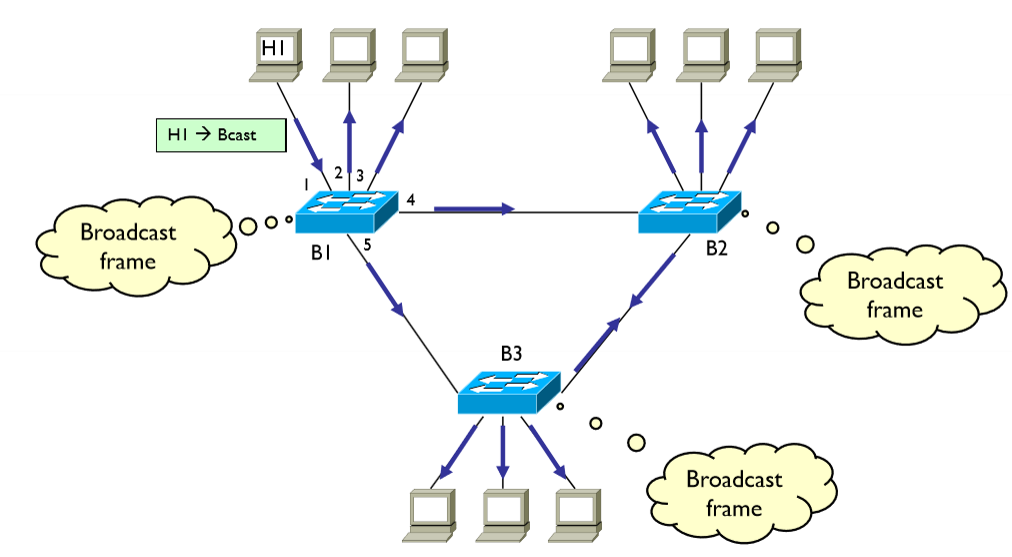
\includegraphics[height=5cm, keepaspectratio]{media/image110.png} 
		\caption{Time 1: Broadcast frame}
		\label{fig:broadcast_stage}
	\end{subfigure}
	\hfill
	% Immagine di destra: Loop
	\begin{subfigure}[b]{0.48\textwidth}
		\centering
		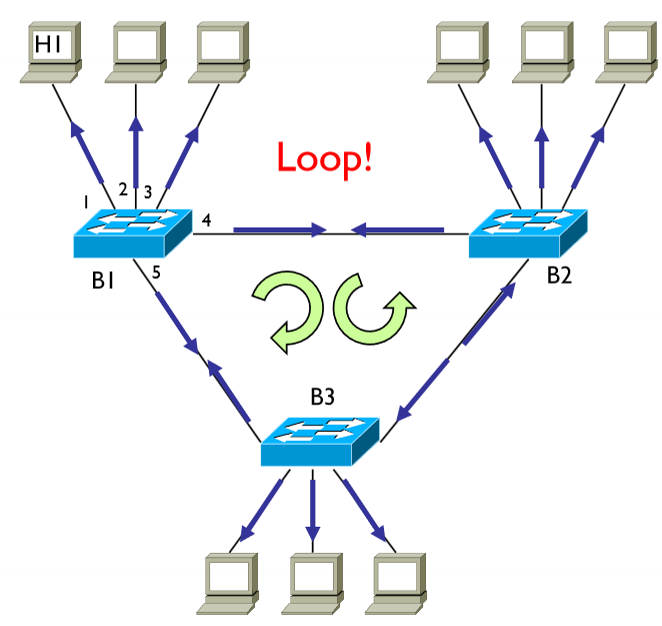
\includegraphics[height=5cm, keepaspectratio]{media/image111.png} 
		\caption{Time 2: Loop!}
		\label{fig:loop_stage}
	\end{subfigure}
	\caption{Comparison between the initial broadcast forwarding and the critical network evolution over time.}
	\label{fig:network_comparison}
\end{figure}

Multicast frames, which are less common in IPv4, are much more common in IPv6, so they contribute significantly to storms. Consider three bridges $B_1$, $B_2$ and $B_3$ interconnected in a triangle, with $H_1$ connected to $B_1$. When $H_1$ sends a broadcast frame, $B_1$ floods it on all ports except the receiving one, so a copy reaches $B_2$ and a copy reaches $B_3$. Each of them replicates it on its other ports and towards the other bridge; when $B_2$ and $B_3$ receive the copies coming from each other, they cannot recognize them as copies of a frame already received, since the Ethernet frame carries nothing that identifies it, and they flood them again towards $B_1$, which replicates them once more. The loop never stops unless one of the links is physically disabled.

A frame sent to a non-existing station loops for the same reason, but with a different cause: since that station never sends frames, its MAC address is never learned, and every switch keeps flooding the frame. This differs from the transient of a new switch, where entries are eventually learned as soon as the hosts send frames; typically, this situation occurs under an attack, such as the one with random destination MAC addresses described above.




This happens because the Ethernet header lacks a Time-To-Live (TTL) field. The inability to naturally discard looping frames at Layer 2 was historically one of the primary motivations for the creation of the IP protocol, which introduced the TTL (or Hop Limit) mechanism specifically to solve this issue at Layer 3.

Because of this structural limitation, a Layer 2 broadcast storm is exceptionally dangerous: it will rapidly consume all available bandwidth and switch CPU resources, inevitably bringing the entire LAN to a halt until the physical loop is broken or algorithmically blocked by STP
\subsection{Learning inconsistencies}

In a looped topology, backward learning may cause MAC entries to change ports repeatedly. When frames traverse the loop, each bridge may update its table incorrectly, causing persistent instability.

For instance, in the triangle of bridges, $B_1$ initially learns $H_1$ on the port towards $H_1$. Suppose the copy of the broadcast frame sent by $B_3$ comes back to $B_1$ before the one sent by $B_2$ (for example because $B_3$ is faster): $B_1$ receives a frame whose source is $H_1$ on the port towards $B_3$ and updates the entry, as if $H_1$ had moved, which is not true. A frame later sent by another host to $H_1$ would then be forwarded towards $B_3$, which is wrong. Shortly after, the copy coming from $B_2$ changes the entry again, and the entry keeps alternating between the two ports for as long as new copies arrive. The same happens in $B_2$ and $B_3$: besides saturating the bandwidth, the storm makes every bridge lose a correct view of the network. Since the two problems are connected, solving the loop solves both.

\section{Introduction to spanning tree}

To prevent loops, bridges implement the spanning tree algorithm. The algorithm identifies a subset of the physical topology that forms a loop free tree. Links not belonging to the spanning tree are disabled for data traffic. Broadcast and multicast frames propagate through the active tree, ensuring freedom from loops.

Routers, in contrast, separate broadcast domains and do not forward link layer broadcasts. They rewrite MAC addresses on forwarded frames and operate at the network layer. Different IP networks must be assigned to a router's interfaces to ensure correct forwarding semantics.


This logical disabling of links explains why STP is strictly suited for LANs and not WANs: in a WAN, automatically disabling an expensive intercontinental fiber-optic link to prevent loops would be an unacceptable waste of financial resources. In campus LANs, however, loops are often intentionally introduced by administrators to provide physical redundancy; if an active link fails, STP automatically detects the failure and restores the usage of a previously disabled link without requiring human intervention.

\begin{center}
	\safeimg[width=4.54306in,height=2.25278in]{media/image112.png}
\end{center}


The Spanning Tree Protocol (STP) is a protocol in its own right, through which the bridges interact with each other and decide, automatically, which link to disable logically; the choice is the result of an election among the bridges, based on the topology they discover. In the triangle example, the link between $B_2$ and $B_3$ could be disabled: broadcast frames, multicast frames and frames sent to non-existing stations are still flooded, but only along the remaining links, so they can no longer loop. Not all switches support STP, and the protocol exists in several variants (for example the Rapid Spanning Tree Protocol). It is a rather complex protocol, and its details are outside the scope of this course.

\section{Layer 2 versus layer 3 in campus networks}

\subsection{Considerations on protocol layer choice}

Until this point, the discussion has focused primarily on layer 2 mechanisms. A fundamental design question in campus networks concerns whether communication should remain at layer 2 or transition to layer 3.

Layer 2 operation provides transparency: end systems can communicate independently of their physical location within the LAN, and the network accommodates any protocol encapsulated in Ethernet frames. Layer 3 operation ties addressing to topology. Hosts receive IP addresses that depend on their position in the network, and many policies such as access lists and firewall rules are bound to the assigned IP prefixes.

When a device is moved from one network to another, at layer 3 its IP address changes, because it depends on its position, and routing tables may have to be updated; at layer 2 the MAC address is preserved, and backward learning simply updates the port in the filtering databases. Moreover, every function whose behavior depends on IP addresses must be updated whenever addresses change. For instance, a packet filtering firewall decides whether a packet is dropped by looking at the IP five-tuple, whose main elements are the source and destination IP addresses, so its access control list must be modified when a host receives a new address; the same holds for other access control functions, intrusion detection systems and, in general, any network security function based on IP addresses.


Furthermore, an L2 infrastructure natively works with any network protocol, allowing organizations or research laboratories to easily deploy and test experimental protocols (as was done during the early development of IPv6) without requiring hardware or routing software upgrades.

\section{Single versus multiple LANs in a campus}

\subsection{Motivation for multiple LANs}

It is generally preferable to maintain layer 2 operation as long as feasible. However, a single unified LAN may become impractical due to scalability constraints inherent in layer 2 networks.

Several issues motivate the subdivision of a campus into multiple LANs:

\begin{itemize}
\item \emph{performance}: broadcast traffic is not filtered by switches, so a single large broadcast domain can experience excessive broadcast or flooded traffic, especially during spanning tree reconfigurations;
\item \emph{privacy and security}: isolation between groups of users is desirable to contain potential information leakage or mitigate attacks such as MAC flooding;
\item \emph{management}: smaller networks are easier to administer, and per group or per department policies can be applied uniformly.
\end{itemize}

These motivations follow the divide-and-conquer paradigm (\emph{divide et impera}): it is better to have several smaller LANs, each independently managed, than a single large one. For instance, if a MAC flooding attack, or a flow of frames with random destination MAC addresses, targets a single large LAN, all its switches are affected; if the network is divided into several LANs interconnected by routers, the attack only affects the switches of the targeted LAN.

\subsection{Physical separation versus virtual segmentation}

One approach to creating multiple LANs is to deploy physically separate networks. If \(N\) LANs must span \(M\) rack rooms, the number of required switches becomes \(N \times M\), and the number of interconnecting links becomes \(N \times (M - 1)\). This strategy wastes resources and complicates maintenance.

To solve the single broadcast domain problem, the classic solution consists of dividing the network into separate subnets and assigning dedicated hardware (separate switches) to each department.

If a commercial switch has 24 or 48 physical ports but a department only has 4 or 5 hosts, most of the switch's physical ports remain unused. Multiplying this scenario for each department, infrastructure costs and hardware waste become unsustainable.

Virtual LANs provide a more efficient alternative.

\section{Virtual LANs}
\subsection{Concept and motivation}

A Virtual LAN (VLAN) allows multiple logical LANs to coexist on a single physical network infrastructure. The same switches and cabling can support multiple departments or groups while dividing the network into separate, logically isolated broadcast domains.

\begin{center}
	\safeimg[width=4.54306in,height=2.25278in]{media/image93.png}
\end{center}

VLAN membership is determined by the configuration of switch ports rather than by physical wiring. From a logical perspective, each VLAN behaves as an independent and isolated transparent bridge, maintaining its own separate filtering database and broadcast domain, while sharing the underlying physical hardware with other VLANs

Main advantages:

\begin{itemize}
\item \textbf{Infrastructural efficiency:} VLANs maximize the utilization of physical switch ports. For example, a single 48-port switch can serve multiple departments simultaneously, avoiding the need for dedicated physical switches for each group.

\item \textbf{Reduced backbone complexity:} Multiple VLANs can share the same physical backbone infrastructure, eliminating the need for multiple parallel backbone links dedicated to separate LANs.

\item \textbf{Broadcast domain isolation:} Broadcast frames generated by a host remain confined to its own VLAN and are not forwarded across VLAN boundaries. This reduces unnecessary broadcast traffic between departments.

\item \textbf{Layer 2 security and isolation:} VLANs limit the scope of certain Data Link layer attacks, such as MAC flooding and ARP spoofing (ARP poisoning). These attacks are generally confined to the affected VLAN and do not automatically propagate to other VLANs. However, VLANs alone do not guarantee complete security and must be combined with appropriate network security mechanisms.

\item \textbf{Organizational flexibility:} Users can be assigned to different logical networks independently of their physical location. For example, when a user moves to another office, the switch port can be reconfigured to assign the user to the same VLAN, without requiring changes to the physical cabling infrastructure.

\end{itemize}

Overall, VLANs provide logical network segmentation over shared physical infrastructure, improving resource utilization, reducing broadcast traffic, simplifying network design, and enabling flexible network administration.

\subsection{VLAN aware switch architecture}

A VLAN-aware switch maintains conceptually separate filtering databases, one for each VLAN. Each database associates MAC addresses with the local switch ports through which the corresponding devices can be reached within that VLAN. Backward learning is also performed independently for each VLAN, so information learned from a frame belonging to one VLAN does not modify the filtering database of another VLAN.

This logical separation is essential because VLANs represent distinct broadcast domains even when they share the same physical switches and cabling infrastructure. Consequently, a switch must identify the VLAN to which an incoming frame belongs before applying backward learning and forwarding decisions.
\begin{center}
	\safeimg[width=4.54306in,height=2.25278in]{media/image94.png}
\end{center}

In practical implementations, the filtering database is often a unified hardware table, frequently implemented using ternary content addressable memory. Entries include additional fields that identify the VLAN context.

\subsubsection{Filtering Databases and Forwarding in VLANs} 

Furthermore, the Spanning Tree Protocol (STP) computes a loop-free subset of the network topology. The following example illustrates how a VLAN-aware switch forwards frames between hosts belonging to the same VLAN while preventing direct Layer 2 communication between different VLANs.

\begin{center}
	\safeimg[width=5.54306in,height=3.25278in]{media/image113.png}
\end{center}

Consider the image before ,the network composed of two switches and six hosts, divided into three VLANs represented by green, yellow, and pink. The hosts are paired as follows: H1 and H4 belong to the green VLAN, H2 and H5 belong to the yellow VLAN, and H3 and H6 belong to the pink VLAN.

Each switch maintains a separate filtering database for each VLAN. When switch 1 receives a frame from H1 destined for H4, it identifies the frame as belonging to the green VLAN and consults only the green filtering database. Since H4 is associated with the appropriate output port in that database, switch 1 forwards the frame through that port. The next switch performs the same operation using its own green filtering database and forwards the frame toward H4. The destination is therefore reached without consulting the databases associated with the other VLANs.

Now suppose that H1 sends a frame destined for H6. Switch 1 again identifies the VLAN associated with the incoming frame and consults only the corresponding filtering database. The entry for H6 is not available in that VLAN's database because H6 belongs to the pink VLAN. The switch must not use the pink database to forward a frame that belongs to another VLAN. Consequently, the frame cannot reach H6 through Layer 2 forwarding.

This behavior is intentional: a VLAN defines a separate broadcast domain, and Layer 2 frames cannot cross VLAN boundaries directly. Communication between different VLANs requires an intermediate Layer 3 device, such as a router.

Without inter-VLAN routing, the only communicating host pairs in this example are H1–H4, H2–H5, and H3–H6. Other pairs belong to different VLANs and cannot communicate directly at Layer 2.

Although these filtering databases are logically independent, they do not necessarily require physically separate memory devices. In practical switches, entries may be stored in a common hardware table, with additional information identifying the VLAN associated with each entry. The switch uses this VLAN context to access the appropriate logical database and preserve traffic isolation.

\section{Interconnecting VLANs}

\subsubsection{Layer 2 separation}

Layer 2 frames do not cross VLAN boundaries. A host cannot send a link layer frame directly to a station in another VLAN. As VLANs define separate broadcast domains, flooded and broadcast traffic remains confined. Therefore, VLANs require a layer 3 device for interconnection.

Broadcast domains cannot be separated by repeaters, nor by switches, but only by routers. Since VLANs are separate broadcast domains, layer 2 frames cannot cross from one VLAN to another without an intermediate network layer device.

This behavior enforces the fundamental rule of VLANs: a Data Link frame can never pass directly from one VLAN to another within an L2 switching infrastructure. If a host attempts to send an L2 frame directly to a device in a different VLAN, the switch consults only the filtering database of the ingress VLAN, fails to find the destination MAC address in that specific context, and either discards the frame or floods it exclusively within the source VLAN.

\subsection{Inter-VLAN routing}
Inter VLAN communication requires a router or a device with equivalent layer 3 forwarding capability. In a traditional approach, every VLAN requires a dedicated physical switch port connected to a separate physical router interface, leading to severe port wastage and poor scalability.


\begin{center}
	\safeimg[width=4.54306in,height=2.25278in]{media/image95.png}
\end{center}

The main limitation of the traditional approach is the number of physical switch ports reserved for the router. For example, watching the image above, consider a 16-port switch that must support 10 VLANs. If one dedicated port is required for each VLAN, 10 of the 16 ports must be reserved for connections to the router, leaving only 6 ports available for other connections. This represents a significant waste of resources. By contrast, if the switch manages only two VLANs, dedicating two ports to the router may be an acceptable solution.

An alternative is the one-arm router, also known as router-on-a-stick. In this configuration, a single physical link connects the switch to one router interface, reducing the number of reserved switch ports. However, because frames belonging to different VLANs arrive through the same physical interface, the router cannot identify the VLAN solely from the incoming port. It must use additional information carried by the frames, typically VLAN tags, to distinguish the different VLANs.

The router can configure multiple logical subinterfaces on the same physical interface, assigning a different IP address to each subinterface. Each subinterface acts as the Layer 3 gateway for its corresponding VLAN. This solution reduces physical port consumption but increases configuration and management complexity because multiple logical interfaces and IP addresses must be maintained on a single physical connection.

When routing traffic between VLANs, the router examines the destination IP address, decapsulates the incoming layer 2 frame, and completely constructs a new frame. This process includes generating new source and destination MAC addresses (where the source becomes the router's interface MAC and the destination belongs to the final target host) and applying the appropriate 802.1Q VLAN tag before re-injecting the frame back onto the shared trunk link.

\subsubsection{VLANs and IP addressing}
Because ARP broadcasts and other discovery protocols cannot cross VLAN boundaries, each VLAN must correspond to a distinct IP subnet. Hosts belonging to different VLANs require addresses from different IP prefixes. Consequently, assigning overlapping IP subnets to different VLANs constitutes a severe design error, as Layer 2 forwarding rules will block direct communication even if hosts appear to share the same logical subnet prefix. 

\begin{center}
	\safeimg[width=3.84306in,height=1.65278in]{media/image114.png}
\end{center}

Inter VLAN routing is then performed according to standard IP forwarding rules, relying on the router's subinterfaces as the default gateways for each respective network segment.

\section{Association of frames to VLANs}

\subsection{VLANs on a single switch}
When VLANs exist only within a single switch, the simplest method to associate incoming frames with VLANs is port-based assignment (also known as static VLANs). Each port is statically configured to belong to a specific VLAN, defining its Port VLAN ID (PVID). Incoming untagged frames are assigned by the switch to the VLAN configured on that port. This method requires no changes to end hosts, which remain completely transparent to the underlying logical segmentation.

\begin{center}
	\safeimg[width=4.54306in,height=2.25278in]{media/image96.png}
\end{center}


For example, suppose H1 and H3 are connected to the same VLAN-aware switch but their access ports are assigned to different VLANs. When H1 sends a frame addressed to H3, the switch associates the incoming frame with the VLAN configured on H1's port. It then consults only the filtering database of that VLAN. Even if H3 is connected to the same physical switch, the frame cannot be forwarded directly to H3 if H3 belongs to another VLAN. This illustrates that VLAN membership is determined by the switch configuration, rather than simply by physical connectivity.
\subsection{VLANs across multiple switches}

When VLANs span multiple switches, frames must be identifiable across inter switch links. A single physical link may carry traffic of multiple VLANs. Similarly, servers, routers, or other devices may belong to more than one VLAN and must be able to transmit VLAN tagged frames.

An inter-switch link cannot be treated as a regular access port assigned to a single VLAN when it must carry traffic belonging to multiple VLANs. If the link were assigned to only one VLAN, frames belonging to other VLANs would not be correctly associated with their respective broadcast domains. Assigning an additional VLAN to the same untagged link would not solve the problem, because the receiving switch identifies untagged frames according to the VLAN configured on the ingress port. Therefore, the link between switches must use VLAN tagging to preserve the identity of each frame's VLAN. The same requirement applies to servers and routers that need to communicate with multiple VLANs through a single physical interface.
\begin{center}
	\safeimg[width=4.54306in,height=2.75278in]{media/image97.jpg}
\end{center}

 To support these scenarios, a tagging mechanism is required. On the other hand, if inter-switch links are misconfigured—such as connecting two switches using Access ports set to different VLANs—no tags are used. This causes a dangerous security flaw called VLAN leaking, where computers from different VLANs accidentally communicate at Layer 2.

\subsection{IEEE 802.1Q tagging}

IEEE 802.1Q specifies an extension of the Ethernet frame format that inserts a 4 byte tag between the source MAC address and the EtherType or length field. 

\begin{center}
	\safeimg[width=3.54306in,height=1.75278in]{media/image98.png}
\end{center}


The tag contains:

\begin{itemize}
	\item \textbf{the Tag Protocol Identifier (TPID)}, set to the hexadecimal value 0x8100 to indicate an 802.1Q framed packet;
	\item \textbf{the Priority Code Point (PCP)} or user priority field (3 bits) for Layer 2 Quality of Service (CoS);
	\item \textbf{the Drop Eligible Indicator (DEI)} or CFI (1 bit) used for congestion management;
	\item \textbf{a 12-bit VLAN identifier (VID)} in the range 1 to 4094 (with 0 and 4095 reserved).
\end{itemize}

The EtherType value 0x8100 indicates that a VLAN tag follows. Tagged frames are therefore 4 bytes longer than standard untagged frames.

\begin{center}
	\safeimg[width=4.54306in,height=2.75278in]{media/image99.png}
\end{center}

Tagging is used only on links that transport multiple VLANs, such as inter-switch connections (trunk ports) or connections to servers, hypervisors, and routers that require membership in several VLANs. End-user devices (PCs) remain untagged at the edge, relying on the switch to add or strip tags transparently.

VLAN tagging is generally used in the network backbone, particularly on trunk links connecting switches, while ordinary end hosts usually exchange untagged Ethernet frames. This design choice preserves the transparency of the switching infrastructure: end systems can communicate without needing to know how VLANs are implemented internally.

The switches add, interpret, and remove VLAN tags when necessary, so that the endpoints can operate without managing VLAN identification themselves. If an endpoint generates tagged frames, it must be aware of the VLAN tagging mechanism and participate in the assignment process. This breaks the transparency normally provided by the switches.

Therefore, the design involves a trade-off. Keeping frames untagged at the network edge simplifies endpoint configuration and preserves transparency, whereas tagging is necessary on links that must carry traffic belonging to multiple VLANs. Some devices, particularly servers and one-arm routers, must generate and process tagged frames because they participate in several VLANs through a single physical connection.
\section{Port types}

\subsection{Access ports}

Access ports send and receive untagged frames, and they represent the default configuration mode for VLAN-aware switches. They are typically used at the edges of the local area network to connect end devices (such as PCs or printers) in order to preserve network transparency as much as possible. Incoming traffic is associated with the VLAN configured on the port, and end systems do not need to modify their frame format.


The VLAN assignment configured on access ports is local to each switch and does not propagate to other switches. However, using access ports on links that must carry multiple VLANs (such as inter-switch links) leads to misconfigurations where frames remain untagged across switches, causing unexpected communication between different VLANs.


\begin{center}
	\safeimg[width=3.54306in,height=1.75278in]{media/image100.png}
\end{center}
Consider two switches connected through access ports. The access port on switch 1 is assigned to VLAN 1, whereas the corresponding access port on switch 2 is assigned to VLAN 5. Suppose H1 is connected to switch 1 and H4 is connected to switch 2.

Although the two access ports have different VLAN assignments, these assignments are local to their respective switches. When H1 sends an untagged frame toward H4, switch 1 associates it with VLAN 1. The frame crosses the inter-switch link without a VLAN tag, because the link is configured as an access connection. Switch 2 receives the untagged frame and associates it with VLAN 5, according to its own local configuration.

Consequently, H1 may communicate with H4 even though the two hosts were intended to belong to different VLANs. This is an example of VLAN leaking, caused by an incorrect inter-switch configuration. To preserve VLAN separation across multiple switches, inter-switch links carrying several VLANs must be configured as trunk ports, so that each frame retains its VLAN identity.

\subsection{Trunk ports}

Trunk ports carry tagged frames and must be configured explicitly, as they are not the default mode. They are used for inter-switch connections (the network backbone) or for advanced devices that participate in multiple VLANs. A trunk port may transport traffic belonging to a configurable set of VLANs simultaneously by embedding the VLAN ID inside the frame headers.

\begin{center}
	\safeimg[width=3.54306in,height=1.75278in]{media/image101.png}
\end{center}


\section{Methods for assigning hosts to VLANs}

Hosts may be assigned to VLANs in several ways:

\begin{itemize}
	\item port-based VLANs, where each port belongs to a single VLAN and handles untagged edge traffic;
	\item transparent assignment based on static associations between MAC addresses and VLANs;
	\item authentication-based assignment using IEEE 802.1X frameworks;
	\item cooperative assignment, where endpoints themselves generate tagged frames and participate in multiple VLANs.
\end{itemize}

The different VLAN assignment methods have different practical implications.

Port-based assignment is straightforward to configure and is widely used for ordinary end hosts. The switch associates each incoming untagged frame with the VLAN configured on the corresponding access port.

MAC-based assignment relies on static associations between device MAC addresses and VLANs. Although possible, it can be difficult to manage because administrators must maintain the associations as devices are added, replaced, or moved. For this reason, it is generally not the preferred solution.

Authentication-based assignment can use IEEE 802.1X, a mechanism also studied in Information System Security. Although it provides a way to associate devices with VLANs based on authentication, this approach is less commonly encountered in the scenarios considered in this lecture.

Cooperative assignment requires endpoints to generate and process VLAN-tagged frames themselves. This breaks the transparency normally provided by switches because the endpoints must be aware of VLAN identification.

However, cooperative assignment is mandatory for devices such as one-arm routers and servers that must participate in multiple VLANs through a single physical link. These devices need to identify the VLAN associated with each received frame and include the appropriate tag when generating frames for different VLANs. Other clients may also use cooperative assignment in special cases, but this is relatively uncommon; ordinary end hosts typically use access ports and untagged frames.

Devices such as servers or routers (like a one-arm router) that require membership in multiple VLANs must use trunk connections and perform cooperative assignment by generating VLAN-tagged frames.


\section{VLANs and spanning tree}

VLANs and the spanning tree algorithm are conceptually independent, but the spanning tree protocol must account for the network topology in which VLANs operate. Two approaches are possible.

In the first approach, a single spanning tree instance is computed for the entire LAN. When a link is disabled to prevent a Layer 2 loop, it is disabled for all VLANs. Consequently, the same loop-free topology is shared by every VLAN, even if some links could have been used by particular VLANs without creating a loop.

In the second approach, a separate spanning tree instance is computed for each VLAN. In this case, a link may be disabled for one VLAN while remaining active for another. Different VLANs can therefore use different loop-free subsets of the physical topology.

Both approaches are valid. The available options depend on the switch implementation and vendor. For example, the professor notes that Cisco switches use per-VLAN spanning tree in the implementations discussed in the lecture, whereas other switches may also support a single spanning tree instance for the entire LAN.

\begin{center}
	\safeimg[width=3.54306in,height=1.75278in]{media/image102.jpg}
\end{center}
\section{Limitations to VLAN isolation}

VLANs provide logical separation at the frame forwarding and broadcast domain level, but complete full network isolation is never guaranteed because the underlying physical infrastructure and inter-switch trunk links are shared. Consequently, broadcast frames and traffic from multiple VLANs must traverse these shared physical links. Therefore, if a broadcast storm occurs in one VLAN, the massive volume of traffic can saturate the physical bandwidth of the shared links, indirectly affecting and degrading the performance of other VLANs. Similarly, a MAC flooding attack can saturate these shared pathways even though it originates within a single VLAN.

Switches are classified into two main categories: VLAN-aware switches, which support VLAN tagging and frame processing, and VLAN-unaware switches (traditional unmanaged bridges). From an economic standpoint, VLAN-unaware switches are less expensive to produce and easier to manage, which is why they are predominantly used in domestic networks where users lack advanced networking expertise. Low-end consumer switches are frequently VLAN-unaware and may drop tagged frames as oversized.

On the contrary, enterprise environments heavily rely on professional products supporting VLAN tagging. However, it is quite common to find VLAN-unaware switches in corporate networks. Network managers typically deploy only professional equipment, but end users often face physical limitations—such as the necessity to attach multiple hosts to a single network socket—and tend to solve these issues independently by purchasing the cheapest unmanaged switches on the market.

Network administrators must anticipate and manage such scenarios to prevent possible network misbehaviour. However, VLAN-unaware switches can still be utilized effectively at the access layer (e.g., to add new ports), provided that all connected hosts belong to the exact same single VLAN.

In practice, the VLAN-unaware switch is connected to a single port of a VLAN-aware switch, which is configured as an access port marked with the single VLAN ID that represents the whole subnetwork below it. The subnetwork may contain several VLAN-unaware switches: what matters is that all the frames coming from it belong to the same VLAN, regardless of how many unaware switches they have crossed.
\begin{center}
	\safeimg[width=3.54306in,height=1.75278in]{media/image103.png}
\end{center}



VLAN isolation is therefore logical rather than physical. Although broadcast frames are confined to their respective VLANs at the endpoint level, traffic belonging to different VLANs may traverse the same trunk links. The bandwidth consumed by these shared links must account for the aggregate traffic of the VLANs using them.

Consequently, a broadcast storm or a MAC flooding attack originating in one VLAN may saturate shared physical links and indirectly degrade the performance of other VLANs. The other VLANs remain logically separated, but they can still be affected by congestion in the common infrastructure.
\section{Ethernet LAN design considerations}

Campus networks typically consist of an access layer (with switches deployed in rooms or on each floor connecting multiple devices via access ports), distribution layers, and core infrastructure. Trunk links interconnect switches transporting multiple VLANs simultaneously, as well as connecting data center servers. VLAN-unaware devices may appear at the edges but must be properly contained to avoid interfering with overall VLAN separation.

\begin{center}
	\safeimg[width=4.54306in,height=2.75278in]{media/image104.jpg}
\end{center}

Routers are required both for external Internet connectivity and for executing inter-VLAN routing. In typical campus designs, a single core router fulfills a dual role: serving as the default gateway for devices to reach the external network, and providing the necessary Layer 3 interconnectivity for devices belonging to different VLANs. Modern wired LANs are based on full-duplex switched Ethernet, where collision domains no longer exist and medium access control mechanisms such as CSMA/CD are obsolete. Redundant links increase robustness, and a spanning tree protocol maintains loop freedom across the topology.

\begin{notebox}
	\textbf{Exam note.} Exams typically contain an exercise on VLANs: a network topology is given together with the configuration of its ports (possibly an incorrect one) and the student must state which devices can communicate with each other, or how a given port must be configured. In most cases the answer follows directly from reading the figure and the configuration, applying the rules seen in this chapter.
\end{notebox}




\chapter{Quality of Service}

\section{Fundamentals of media coding}

\subsection{From analog signals to digital representations}

Multimedia applications typically involve the transport of audio, images and video over packet networks. These media originate as \textbf{continuous--time analog signals}. Packet networks, however, operate on \textbf{discrete--time, discrete--amplitude} sequences that can be represented and processed digitally.

\textbf{Media coding} encompasses the techniques used to convert analog signals into efficient digital form suitable for storage, processing and transmission. The process consists of two principal stages:

\begin{enumerate}
\item \textbf{Sampling and quantization}, which convert the analog signal into a discrete sequence of numerical samples.
\item \textbf{Coding and compression}, which transform the numerical sequence into a compact bit stream.
\end{enumerate}

The goal is to obtain a digital representation that is compact yet sufficiently faithful to the original signal for the intended application.

\subsection{The media coding pipeline}

Given an analog source, the standard sequence of operations is:

\begin{enumerate}
\item The analog signal is \textbf{sampled} at regular intervals in time (and space for images and video).
\item Each sample is \textbf{quantized} to one of a finite set of amplitude levels.
\item The resulting integers are mapped to binary values to form a digital bit stream.
\item The bit stream is \textbf{encoded and compressed} to reduce redundancy.
\end{enumerate}

Each step influences the perceptual quality of the reconstructed signal as well as the computational and bandwidth requirements.

\section{Sampling and quantization}

\subsection{Sampling of analog signals}

Sampling transforms a continuous--time signal $x(t)$ into a discrete sequence by evaluating it at uniform intervals:

\[ x[n] = x(nT_s), \quad n \in \mathbb{Z}, \]

\noindent where $T_s$ is the sampling period and $f_s = 1/T_s$ is the sampling frequency.

The sampling frequency must be sufficiently high to preserve the essential information of the original signal. If the highest frequency component present is $f_{\max}$, faithful reconstruction requires:

\[ f_s \ge 2 f_{\max}. \]

This lower bound is known as the \textbf{Nyquist rate}. In practice, sampling frequencies are chosen somewhat higher to accommodate imperfections in filtering and signal variability.

For a signal whose significant content lies within a range of frequencies such as 90 Hz to 120 Hz, any valid sampling frequency must exceed twice the largest relevant frequency component. Higher sampling frequencies produce more samples and therefore increase the data rate.

\subsection{Quantization of samples}

After sampling, the resulting real-valued samples must be mapped to discrete amplitude levels for digital representation. A \textbf{quantizer} replaces sample $x[n]$ with a reconstruction value:

\[ \hat{x}[n] = Q(x[n]). \]

A common design is the \textbf{uniform scalar quantizer}, in which the amplitude range is divided into equal-width intervals. Each sample is assigned the reconstruction level associated with the interval containing it.

With $L$ quantization levels, each output sample can be represented using $b = \log_2 L$ bits, assuming $L$ is a power of two. Typical values in audio applications include 8 bits per sample (sufficient for some voice systems) and 16 bits per sample (common for high-fidelity audio).

\subsection{Quantization error and its effects}

Quantization introduces a difference between the original and quantized values:

\[ e[n] = x[n] - \hat{x}[n]. \]

This \textbf{quantization error} acts as noise added to the signal. The error cannot be eliminated, but its magnitude decreases as the number of quantization levels increases.

A widely used metric for evaluating quality is the \textbf{signal-to-quantization-noise ratio} (SQNR). For a uniform quantizer, the average error power scales with the square of the quantization step size. Thus, increasing $b$ reduces the step size and improves the SQNR.

The perceptual impact of quantization depends on both the signal characteristics and human sensitivity. For many signals, especially audio, modest quantization noise may be imperceptible when the quantizer has sufficiently fine resolution.

\subsection{Resolution, bit rate and resource trade-offs}

If the sampling frequency is $f_s$ and the number of bits per sample is $b$, the raw bit rate required to represent the signal is:

\[ R = f_s \cdot b. \]

For example:

\begin{itemize}
\item 44.1 kHz sampling with 16 bits per sample yields approximately 705.6 kbps for a single audio channel.
\item Two channels (stereo) require about 1.41 Mbps.
\end{itemize}

Higher sampling frequency or larger quantization depth improves quality but increases the number of transmitted bits. This fundamental trade-off must be balanced against network constraints and application requirements.

\section{Coding of samples and compression}

\subsection{From raw samples to encoded bit streams}

A naive digital representation stores each quantized sample using a fixed number of bits. This approach ignores statistical and perceptual redundancies present in multimedia signals. \textbf{Compression} techniques exploit these redundancies to reduce the number of bits while maintaining acceptable quality.

In many forms of multimedia:

\begin{itemize}
\item Audio samples exhibit strong temporal correlation.
\item Image pixels display similarity among neighbors.
\item Video frames contain regions that change little over time.
\end{itemize}

By reducing redundancy, compression techniques convert the raw sequence of samples into a compact bit stream that retains perceptually significant information.

\subsection{Lossless and lossy compression}

Compression techniques can be classified as lossless or lossy.

\textbf{Lossless compression} \textbf{Lossless compression} allows exact reconstruction of the original digital samples after decompression. It preserves all information and introduces no distortion.

Characteristics include:

\begin{itemize}
\item Exact recovery of the original signal.
\item Moderate compression factors, since no information may be discarded.
\item Use in contexts where fidelity is critical.
\end{itemize}

Typical methods include entropy coding and dictionary-based schemes.

\textbf{Lossy compression} \textbf{Lossy compression} permits controlled degradation of the reconstructed signal by discarding components that are less perceptually significant.

Characteristics include:

\begin{itemize}
\item Only approximate reconstruction of the original.
\item Potentially very large compression factors.
\item Possible perceptual artifacts if compression is excessive.
\item Common use in consumer audio, image distribution and video services.
\end{itemize}

Designs rely on psychoacoustic or psychovisual models to identify information that can be discarded with minimal perceptual impact.

\subsection{Redundancy in multimedia signals}

\textbf{Spatial redundancy} \textbf{Spatial redundancy} arises from correlations among neighboring spatial samples. In images, large regions often have uniform or slowly varying intensity. Instead of encoding each pixel individually, one may encode:

\begin{itemize}
\item a representative value,
\item together with the number of repetitions.
\end{itemize}

This principle underlies methods such as run-length coding. More advanced techniques apply transforms that concentrate signal energy into fewer coefficients, allowing many coefficients to be quantized coarsely or omitted.

\textbf{Temporal redundancy} \textbf{Temporal redundancy} arises when successive samples in time are similar. Video sequences often contain frames with only small temporal differences.

A predictive strategy involves:

\begin{enumerate}
\item Estimating motion or change between successive frames,
\item Predicting the next frame using this estimate,
\item Encoding only the difference between the predicted and actual frame.
\end{enumerate}

Since the prediction error typically has lower variance than the original frame, fewer bits are required to encode it. Similar predictive ideas apply in audio coding, where samples evolve smoothly in time.

\subsection{Combined spatial and temporal reduction}

Modern codecs jointly exploit spatial and temporal redundancy. In video, for example, spatial transforms may be applied to intra-frame prediction residuals, while temporal prediction reduces inter-frame redundancy. The combined approach yields substantial compression gains while maintaining acceptable perceptual quality.

\section{Networked multimedia applications}

\subsection{Overview of multimedia services in packet networks}

A wide range of modern networked services are based on the transmission of multimedia information. Such services may involve one or multiple forms of media, including audio, images and video. Even applications that employ a single medium typically exhibit characteristics that distinguish them from traditional data services. Representative examples include information retrieval platforms, broadcast services, on-demand video distribution, telephony, real-time conferencing, interactive gaming, distance learning environments and immersive virtual reality systems.

These applications impose requirements that differ substantially from those associated with conventional best-effort data transfer. Their operation relies on sustained information flows, real-time constraints, interactivity and often communication among groups of users. The combination of these characteristics necessitates careful consideration of the behaviour of packet networks under load.

\subsection{Distinctive characteristics of multimedia traffic}

\subsubsection*{Streaming}
\addcontentsline{toc}{subsubsection}{Streaming}

Multimedia applications frequently generate a \textbf{continuous flow of data}. Unlike applications such as electronic mail or traditional web browsing, which produce data sporadically, multimedia streams generate traffic at regular intervals that must be preserved during transport.

If samples are produced at specific temporal intervals, then the received stream must adhere to the same temporal structure. For instance, if a system generates one sample every 125 microseconds, the playback subsystem must receive and process samples at an equivalent rate to maintain uninterrupted output. Deviations from this profile disrupt playout and may cause buffer underflow, loss of continuity or temporal artifacts.

\subsubsection*{Interactivity}
\addcontentsline{toc}{subsubsection}{Interactivity}

Traditional data applications provide limited interactivity, typically involving long response times or asynchronous communication. By contrast, multimedia applications often require \textbf{rapid and bidirectional interaction}. Users may interact with other humans, automated systems or both.

High interactivity demands short response times, as delays perceptible to users degrade the quality of experience. In conversational scenarios, excessive response time leads to repeated interruptions, misalignment of dialog and reduced usability. Consequently, underlying networks must support low-latency communication paths.

\subsubsection*{Large bandwidth and group communication}
\addcontentsline{toc}{subsubsection}{Large bandwidth and group communication}

Many forms of multimedia require \textbf{substantial transmission bandwidth}. High-definition video, interactive gaming and immersive virtual environments are particularly demanding due to the large volume of data generated per unit time.

In addition, numerous multimedia applications rely on \textbf{group communications}. These may involve one-to-many or many-to-many exchanges, where the same content must be conveyed to multiple recipients. Efficient support for such communication patterns is crucial to avoid redundant transmissions and excessive load on the network.

\section{Requirements imposed by multimedia applications}

\subsection{Requirements associated with streaming}

Proper support for streaming demands that the network exhibit \textbf{limited packet loss}. Although multimedia systems often tolerate a moderate degree of loss, excessive loss introduces perceptual degradation and may interrupt continuity. Additionally, streaming requires \textbf{low jitter}, defined as the variability in packet delay.

If delay variability is significant, the temporal structure of the arriving data is distorted relative to the original. Compensation techniques can be applied, such as delaying early packets until late packets arrive, but these increase the end-to-end delay and may be unacceptable for interactive scenarios.

\subsection{Requirements associated with interactivity}

Interactive multimedia applications require \textbf{low one-way delay}. Human verbal interaction typically becomes impaired when one-way delays exceed approximately 100--150 ms, leading to conversational overlap and repeated interruptions.

In packet networks, excessive delay often originates in congestion within router buffers. When multiple packets contend for the same output interface, queuing occurs, and routers must temporarily store packets. Since buffering increases delay, and since delays fluctuate with instantaneous queue occupancy, networks must regulate queuing to meet interactive requirements.

\subsection{Requirements associated with high bandwidth}

High-bandwidth multimedia applications require substantial \textbf{transmission capacity}, \textbf{buffer space} in intermediate nodes and \textbf{processing power} for operations such as routing and scheduling. The feasibility of supporting such applications depends heavily on network architecture and technology. Improvements in physical-layer capabilities and router hardware directly enhance the ability of networks to support bandwidth-intensive multimedia workloads.

\subsection{Requirements associated with group communication}

Multimedia systems involving multiple participants benefit from \textbf{multicast transmission services}. Efficient mechanisms, such as network-layer multicasting, enable data to be replicated within the network rather than at the source, thereby reducing redundant transmissions. Additional architectural elements, such as reflectors or multipoint control units, may be employed to manage and distribute group communication traffic effectively.

\section{Delay and its implications for multimedia systems}

\subsection{The nature of delay in multimedia communication}

Multimedia applications are inherently \textbf{real-time} in the sense that the timing of results is as important as the correctness of the data conveyed. Delays must be bounded and controlled, although they need not necessarily be minimal in all cases. The defining requirement is that delay remain predictably within the limits acceptable for the specific application.

\subsection{Variability of delay}

Packet delay varies with the \textbf{instantaneous load} at network nodes. When multiple packets arrive at a router interface and compete for transmission, some must be buffered, introducing additional queuing delay. As queue lengths fluctuate with traffic intensity, the resulting delay varies over time. This variability complicates the maintenance of consistent playout timing at the receiving end.

\section{Countermeasures for supporting multimedia traffic}

\subsection{Countermeasures implemented in end systems}

End systems may employ several techniques to mitigate network-induced impairments:

\begin{itemize}
\item \textbf{Compensation for delay variation}. Incoming data units can be buffered so that all units are subjected to a controlled maximum delay. While this stabilizes playout timing, it increases end-to-end delay and may become problematic for interactive applications.
\item \textbf{Adaptation to network conditions}. Applications may adjust their sending rate or encoding parameters in response to observed quality degradation. Such adaptability is constrained by content characteristics and user requirements.
\end{itemize}

\subsection{Countermeasures implemented within the network}

Networks themselves may deploy techniques to provide improved support for multimedia traffic:

\begin{itemize}
\item \textbf{Traffic classification}, which identifies packets belonging to specific applications or traffic classes. Although classification alone does not provide guarantees, it is essential for enabling differentiated treatment.
\item \textbf{Advanced scheduling algorithms}, which determine the order in which packets are transmitted. Traditional FIFO queuing is insufficient for applications requiring quality of service, and more sophisticated policies must be used to ensure predictable behaviour.
\item \textbf{Control of traffic entering the network}, achieved through admission control and policing mechanisms, which prevent excessive queue occupancy and mitigate congestion.
\end{itemize}

\section{Quality of service support}

Effective support for multimedia applications requires the combined use of all three categories of countermeasures. Networks must limit the volume of incoming traffic so that nodes do not become overloaded, and must handle appropriately any flows requiring specific performance guarantees. These coordinated measures collectively enable the delivery of multimedia content with the quality constraints imposed by real-time and interactive applications.

\section{Quality of service support: classification}

\subsection{Purpose of classification}

Quality of service mechanisms rely on the ability of the network to distinguish among different traffic flows. \textbf{Classification} is the operation that identifies the flow to which each incoming packet belongs and determines the queue in which that packet must be stored. By separating packets into distinct queues, the network can apply differentiated scheduling and forwarding policies, thereby ensuring that flows requiring specific performance properties receive appropriate treatment.

\begin{center}
\safeimg[width=4.42917in,height=2.3in]{media/image18.png}
\end{center}

Packets belonging to applications with stringent delay or jitter constraints may be assigned to queues with higher priority, while elastic or background traffic may be placed in lower-priority queues. The classification step therefore plays a foundational role in enabling differentiated handling of heterogeneous traffic.

\subsection{Basis for classification}

Classification typically relies on information carried in protocol headers. A widely used approach is based on the \textbf{IP five-tuple}, which consists of:

\begin{itemize}
\item destination IP address,
\item source IP address,
\item transport protocol,
\item destination port,
\item source port.
\end{itemize}

This combination uniquely identifies most unicast flows in modern networks.

Traditional routers examine only a limited subset of header fields, primarily the destination IP address and ancillary fields such as the time-to-live. However, routers designed to support quality of service may also inspect dedicated fields intended for differentiated treatment. An example is the \textbf{Type of Service} field in the IP header, which can encode priority or service class information.

\subsection{Complexity and hardware support}

Classification is computationally intensive because it requires examination of transport-layer fields in addition to network-layer information. The lookup string, often including five distinct header components, can be long, and matching each packet against potentially numerous flow specifications constitutes a nontrivial operation.

Owing to these demands, classification is commonly implemented in specialized hardware. Two prominent technologies are:

\begin{itemize}
\item \textbf{Application specific integrated circuits (ASICs)}, which provide high-speed packet processing tailored to classification and forwarding tasks.
\item \textbf{Content addressable memory (CAM)}, in which memory locations are identified by their content rather than by an address. CAM structures permit rapid matching of header fields against stored patterns, enabling packet classification at line rate.
\end{itemize}

These hardware mechanisms ensure that classification does not become a bottleneck, even in high-speed routers supporting large numbers of simultaneous flows.

\section{Quality of service support: packet scheduling}

\subsection{Traditional queuing}

Packet scheduling governs the order in which queued packets are transmitted over an output link. The simplest mechanism is \textbf{first-in first-out} (FIFO) queuing, where packets are transmitted strictly in the order of arrival. This method treats all flows identically and offers no differentiation based on service requirements.

\begin{center}
\safeimg[width=4.42917in,height=1.64861in]{media/image19.png}
\end{center}

In FIFO systems, the output link is shared dynamically among multiple flows through statistical multiplexing. As packets from different flows interleave, their output timing may deviate significantly from the timing at which they were originally generated. This variability can degrade the performance of applications that rely on consistent timing, particularly multimedia streams that require steady play-out.

\subsection{Multiple queues and scheduling}

To accommodate heterogeneous traffic requirements, routers often maintain \textbf{multiple queues}, grouping packets according to classification results. Each queue can then be serviced according to a scheduling policy that reflects its priority or bandwidth requirements.

Different classes of traffic can thus be separated, preventing high-volume or delay-tolerant flows from disrupting delay-sensitive or priority traffic. Scheduling algorithms define how the router alternates among these queues when selecting the next packet to transmit.

\subsection{Scheduling algorithms}

Various scheduling mechanisms have been developed to provide differentiated performance guarantees while controlling delay, jitter and fairness. Common algorithms include priority queuing, round robin, weighted round robin, fair queuing and weighted fair queuing.

\subsubsection*{Priority queuing}
\addcontentsline{toc}{subsubsection}{Priority queuing}

In \textbf{priority queuing}, each queue is assigned a fixed priority level. The scheduler always serves the highest-priority nonempty queue before considering lower-priority queues. This approach ensures rapid service for critical traffic but can lead to \textbf{starvation} of lower-priority queues if high-priority traffic persists.

\begin{center}
\safeimg[width=4.42917in,height=1.64861in]{media/image20.png}
\end{center}

\subsubsection*{Round robin scheduling}
\addcontentsline{toc}{subsubsection}{Round robin scheduling}

\textbf{Round robin} scheduling cycles among queues, taking one packet from each queue in sequence. All queues are treated equally, making this method simple and inherently fair under the assumption that all packets have similar size.

\begin{center}
\safeimg[width=4.42917in,height=1.64861in]{media/image21.png}
\end{center}

However, since packet sizes vary in practical networks, round robin may allocate unequal amounts of bandwidth to different queues. A queue containing larger packets consumes more transmission time per scheduling round, producing unfair service distribution.

\subsubsection*{Weighted round robin}
\addcontentsline{toc}{subsubsection}{Weighted round robin}

\textbf{Weighted round robin} addresses this limitation by assigning a weight to each queue. During each scheduling cycle, the scheduler transmits a number of packets proportional to the weight of each queue. A queue with weight $w$ may transmit $w$ packets per cycle, allowing differentiated service levels among classes while retaining the simplicity of round-based scheduling.

Although weighted round robin improves fairness relative to round robin, the algorithm still operates on packet counts rather than transmission time. When packet sizes vary, queues with larger packets may receive disproportionately more bandwidth than intended.

\begin{center}
\safeimg[width=4.42917in,height=1.64861in]{media/image22.png}
\end{center}

\begin{center}
\safeimg[width=4.42917in,height=1.44444in]{media/image23.png}
\end{center}

\subsubsection*{Fair queuing}
\addcontentsline{toc}{subsubsection}{Fair queuing}

\textbf{Fair queuing} aims to give each traffic class an equal share of the output link bandwidth by scheduling packets based on the amount of service received rather than on packet counts. The scheduler conceptually emulates bit-by-bit round robin service among queues, approximating perfect fairness even in the presence of variable packet sizes.

\begin{center}
%\safeimg[width=4.42917in,height=1.44444in]{media/image24.png}
\end{center}

In practice, fair queuing computes a virtual finish time for each packet based on its length and the service history of its queue. Packets are then transmitted in order of increasing finish time, ensuring that each class receives an equitable fraction of the available bandwidth.

\subsubsection*{Weighted fair queuing}
\addcontentsline{toc}{subsubsection}{Weighted fair queuing}

\textbf{Weighted fair queuing} generalizes fair queuing by allocating bandwidth shares proportional to assigned weights. A class with weight $w$ receives a fraction of service proportional to $w$, enabling sophisticated quality of service differentiation while preserving fairness among queues of equal weight.

\begin{center}
%\safeimg[width=4.42917in,height=1.44583in]{media/image25.png}
\end{center}

Weighted fair queuing is considered an idealized scheduling discipline because it offers strong fairness, predictable delay bounds and precise bandwidth allocation. However, its practical implementation is complex due to the need for continuous estimation of virtual service times and dynamic queue state management.

\section{Quality of service support: traffic control}

\subsection{Traffic control performed a priori}

Traffic control mechanisms may operate before packets enter the network or after they arrive at boundary devices. When performed \textbf{a priori}, traffic control concerns the dimensioning and organization of the network itself.

\subsubsection*{Network engineering}
\addcontentsline{toc}{subsubsection}{Network engineering}

Network engineering defines the physical and logical capacity of a network according to expected traffic demand. The service provider must ensure that the network has sufficient transmission capacity, buffer resources and switching capabilities to sustain the aggregate load. Furthermore, the provider must sell services to customers in a manner consistent with the actual network size, so that demand does not exceed available resources.

\subsubsection*{Traffic engineering}
\addcontentsline{toc}{subsubsection}{Traffic engineering}

Traffic engineering determines how traffic should be distributed across network nodes, given the existing network size and anticipated load. This may involve routing flows along paths that are not the shortest, in order to balance load and avoid congestion. The objective is a controlled allocation of traffic across the network to ensure that no single portion becomes overloaded.

\subsection{Traffic control performed a posteriori}

Traffic control may also be applied after traffic reaches network access points or routers, operating either at the granularity of individual packets or at the granularity of flows.

\subsubsection*{Packet-level control}
\addcontentsline{toc}{subsubsection}{Packet-level control}

Packet-level control mechanisms regulate how many packets from a source are permitted to enter the network. If an application or host exceeds the allowable rate, packets may be delayed, shaped or discarded. Two principal techniques are used:

\begin{itemize}
\item \textbf{Shaping}, which delays packets so that outbound traffic conforms to a target profile.
\item \textbf{Policing}, which enforces conformance by discarding or marking packets that exceed the permitted rate.
\end{itemize}

\subsubsection*{Flow-level control}
\addcontentsline{toc}{subsubsection}{Flow-level control}

At the flow level, resource reservation protocols aim to secure network resources for individual sessions. An example is the \textbf{Resource Reservation Protocol (RSVP)}, which attempts to reserve bandwidth and related resources along the path between a sender and a receiver. Reservations are maintained as \emph{soft state}, requiring periodic refresh messages to remain active. If any router cannot meet the reservation request, it may reject the request entirely or accept it partially.

\subsection{Shaping and policing mechanisms}

Traffic entering the network must conform to a \textbf{traffic profile} consisting of an average bit rate and a maximum burst size. The profile may be requested by the application or determined by the service provider based on network capacity.

\subsubsection*{Token bucket mechanism}
\addcontentsline{toc}{subsubsection}{Token bucket mechanism}

A widely used mechanism for enforcing traffic profiles is the \textbf{token bucket} algorithm. Consider an application that generates traffic at an average rate of 1 MBps with a maximum burst size of 10 MB. Tokens are placed into a bucket at the average rate; for instance, if one token represents one bit, then one token arrives every microsecond. A packet is forwarded only if sufficient tokens exist in the bucket, and the corresponding number of tokens is removed. The bucket size equals the maximum allowed burst.

This algorithm can be employed by:

\begin{itemize}
\item \textbf{network access devices}, where it acts as a policing mechanism;
\item \textbf{end hosts}, where it operates as a shaping mechanism.
\end{itemize}

\section{Quality of service frameworks}

\subsection{Integrated services}

The \textbf{Integrated Services (IntServ)} architecture sought to provide guaranteed QoS for individual flows in IP networks. Conceptually similar to earlier digital communication systems that combined loss-sensitive computer data with delay-sensitive telecommunication services, IntServ introduces per-flow resource reservation.

The Resource Reservation Protocol is used to transmit reservation requests through the network. Each router along the path must determine whether it can satisfy the request. If resources are available, the router admits the flow and guarantees its QoS for the duration of the reservation.

Although the framework is standardized and implemented in routing equipment, it is not practical for large public networks, primarily due to:

\begin{itemize}
\item \textbf{high complexity}, since each router must maintain state for numerous flows and employ sophisticated scheduling algorithms;
\item \textbf{low scalability}, as QoS guarantees can be maintained only for a limited number of flows.
\end{itemize}

\subsection{Differentiated services}

\textbf{Differentiated Services (DiffServ)} adopts a more scalable approach, offering differentiated performance not to individual flows but to a limited number of well-defined traffic classes. DiffServ does not attempt per-flow resource reservation and does not guarantee end-to-end QoS for single applications.

Routers rely on the DiffServ (DS) field in the IP header to classify packets into service classes. Each class receives distinct queueing and forwarding treatment. Individual applications within a class do not receive explicit guarantees, but aggregate behaviour for the class can be managed.

Effective DiffServ operation requires additional traffic control measures, including:

\begin{itemize}
\item network engineering,
\item traffic engineering,
\item access policing at network boundaries.
\end{itemize}

DiffServ achieves:

\begin{itemize}
\item \textbf{simplicity}, because routers need not maintain per-flow state and can rely on simpler scheduling mechanisms;
\item \textbf{scalability}, because a small number of classes is easier to manage than a large number of flows.
\end{itemize}

However, efficiency is limited because the absence of explicit reservations prevents the network from precisely predicting or controlling the amount of generated traffic.

Network operators can only estimate load and provision resources accordingly.

\textbf{Part II} \textbf{Cloud Technologies}

\chapter{Cloud Computing}

\section{Understanding cloud computing}

Cloud computing represents a model for delivering computing capabilities as network-accessible services that can be provisioned dynamically, managed efficiently, and consumed on demand. It has emerged from a long technological evolution that spans networked information systems, distributed computing, and large-scale data center architectures.

The contemporary notion of cloud computing consolidates earlier trends in Internet-based service delivery and draws from innovations in virtualization, resource pooling, and service management. Its conceptual foundations can be traced to developments in both consumer-oriented Internet services and enterprise-level distributed systems.

\subsection{Historical origins}

The conceptualization of cloud-delivered computing services originated in the mid-1990s. Early discussions within the computing industry began to describe the Internet as an abstract computational infrastructure capable of hosting data and applications. This perspective anticipated a shift away from dependence on local personal computers and toward remote service delivery through networked environments.

During this period, widely used Internet platforms provided practical demonstrations of scalable, remotely hosted services. Search engines, web-based e-mail systems, and early social media platforms offered continuous, ubiquitous access to information and applications. Although primarily consumer-oriented, these systems validated the architectural principles that underlie modern cloud infrastructures, including centralized resource management, elastic service availability, and distributed data accessibility.

\subsection{Industrial and commercial developments}

In the late 1990s, enterprise computing began to adopt models for remotely provisioned services. A significant milestone was the introduction of hosted business applications, which provided organizations with centrally managed software accessible through the Internet. This marked one of the first large-scale implementations of the service-based delivery model that later became characteristic of cloud computing.

By 2002, large e-commerce platforms had begun to commercialize service-oriented infrastructures by offering remotely provisioned storage, processing capacity, and programmatic utilities. These early service suites demonstrated that large-scale data center operators could expose their internal computing capabilities to external consumers in a standardized, scalable manner.

The term \textbf{cloud computing} gained widespread recognition in 2006, coinciding with the introduction of virtualized, on-demand compute instances. These services enabled organizations to lease computational capacity without deploying physical hardware, establishing the economic and technological model that now defines cloud computing.

Subsequent years saw rapid expansion of cloud-based enterprise platforms. Browser-based office applications provided evidence that productivity tools could be delivered entirely through web interfaces. Additional cloud platforms reinforced the viability of remote application hosting and execution, further promoting cloud adoption within enterprise environments.

Major global cloud platforms emerged during the late 2000s and early 2010s, offering integrated service ecosystems that encompassed infrastructure, platform, and application delivery. More recently, cloud initiatives within regional and governmental contexts have aimed to establish federated infrastructures designed to meet regulatory, economic, and sovereignty requirements.

\section{Definition of cloud computing}

A widely accepted definition characterizes cloud computing as the provision of shared and configurable computing resources accessible through the network with minimal administrative overhead. This definition emphasizes ubiquity, convenience, on-demand provision, and the ability to elastically adjust resource allocation.

Cloud computing encompasses a broad range of resources, such as networks, servers, storage systems, application components, and complete services. These resources are abstracted and exposed through standardized interfaces that allow rapid provisioning and deprovisioning. The consumer interacts with these resources without managing the underlying hardware or physical infrastructure.

\section{Business drivers for cloud adoption}

Organizations adopt cloud computing in response to technical, economic, and operational factors. Several structural challenges within traditional on-premise computing environments motivate the transition toward cloud-based architectures. Key drivers include capacity planning, cost reduction, control of operational overhead, and the need for organizational agility.

\subsection{Capacity planning}

Capacity planning involves determining how to meet projected demand for an organization's computing resources. Capacity refers to the maximum workload that an information technology resource can support within a specified time interval. Maintaining an appropriate balance between available capacity and workload demand is central to sustaining efficient and reliable system performance.

A mismatch between capacity and demand produces two principal conditions: inefficiency resulting from excess capacity and performance degradation resulting from insufficient capacity. Over-provisioning requires investment in hardware and infrastructure that may remain underutilized. Under-provisioning restricts the system's ability to satisfy workload requirements, which can lead to reduced quality of service, application slowdowns, and business losses.

Estimating future demand is inherently difficult because usage patterns fluctuate over time. Organizations must plan for peak loads without incurring unnecessary costs. When infrastructure is dimensioned solely according to maximum expected demand, financial investments can become disproportionate to average usage levels. Conversely, minimizing investment risks insufficient performance during periods of high demand.

Different strategies exist for adjusting resource capacity in response to foreseeable or actual workload changes. A lead strategy introduces additional capacity in anticipation of increased demand. A lag strategy adds capacity only after existing resources reach saturation. A match strategy incrementally expands capacity as demand grows, aiming to keep resource allocation closely aligned with real-time consumption.

\subsection{Cost reduction}

Cost considerations are central to cloud adoption. Traditional computing environments require substantial upfront investments in hardware procurement and significant ongoing expenses related to managing and operating infrastructure. The performance of any automation solution is bounded by the processing capabilities of the underlying on-premise systems, often necessitating continual investment in capacity expansion.

Cloud computing reduces or eliminates many of these capital expenditures by shifting costs to a consumption-based model in which resources are acquired on demand. This model allows organizations to begin with minimal investment and expand their resource usage proportionally as their computing needs grow. Large cloud providers operate data centers at scales that enable lower real estate, personnel, and bandwidth costs, further reducing the financial burden on individual enterprises.

\subsection{Operational overhead}

Operational overhead encompasses the recurring costs required to maintain and support on-premise information systems. These costs can exceed initial hardware investments, making them a significant component of IT budgets.

Operational overhead includes staffing for equipment maintenance, installation of updates, and application of security patches. It also involves expenditures related to electricity, cooling, facility maintenance, and security controls for physical infrastructure. Administrative resources are required to manage licenses, support contracts, and procurement activities. Cloud computing reduces these overheads by centralizing infrastructure management within the provider's environment.

\subsection{Organizational agility}

Organizational agility denotes the capacity of an enterprise to respond efficiently to changes in its internal or external environment. Traditional on-premise infrastructures can limit this agility because scaling requires capital expenditure, procurement lead times, and extensive planning.

Cloud computing provides flexible resource allocation that enables organizations to adapt quickly to varying workloads, new business requirements, or market conditions. Since cloud-based resources can be provisioned remotely and expanded dynamically, they support rapid scaling with lower financial and operational barriers. This capability aids organizations in maintaining competitiveness and resilience.

\section{Benefits of cloud computing}

Cloud computing introduces structural advantages that affect the economic, operational, and technical dimensions of information systems. These advantages arise from the consolidation of resources within large-scale data centers, from the adoption of on-demand provisioning models, and from the abstraction of infrastructure through standardized service interfaces. Three categories of benefits are commonly identified: reduced investments and proportional costs, increased scalability, and improved availability and reliability.

\subsection{Reduced investments and proportional costs}

A foundational benefit of cloud computing is the reduction or elimination of significant initial expenditures on hardware and software. Traditional environments require organizations to purchase servers, storage devices, networking equipment, licenses, and support contracts before deploying applications. These capital-intensive acquisitions often occur prior to realizing any operational value, and they can impose long-term financial commitments.

Cloud environments transform these capital expenses into operational expenses. Organizations are able to access computing resources without purchasing or owning the underlying infrastructure. This arrangement permits gradual growth, enabling enterprises to allocate minimal resources during initial stages and expand consumption as operational demands increase. The ability to scale financial expenditure in proportion to actual utilization aligns resource costs more closely with business activity.

Large cloud providers achieve economies of scale by operating massive data centers in locations optimized for cost efficiency. Such locations can offer reduced real estate prices, lower utility costs, and access to an abundant pool of skilled IT professionals. As a result, cloud providers can operate infrastructure at a lower cost per computing unit compared to smaller on-premise facilities. These savings transfer to consumers through competitive pricing models.

\subsection{Increased scalability}

Cloud computing supports rapid adjustments to resource allocation. This scalability can occur automatically based on predefined policies or manually in response to operational requirements. The ability to obtain resources on demand allows organizations to respond quickly to fluctuations in workload intensity.

Cloud platforms provide the perception of limitless computational resources. Consumers can request processing power, memory, storage, and network bandwidth with minimal delay, often within seconds. Resources can also be released immediately when no longer needed, avoiding the costs associated with maintaining idle capacity. This elasticity reduces the need for extensive planning and over-provisioning, which are common in traditional environments where infrastructure must be sized for peak usage.

Fine-grained scaling is another important characteristic. For example, storage capacity can be increased or decreased in small increments, allowing organizations to align resource consumption precisely with real-time demand. This eliminates the inefficiencies caused by coarse-grained capacity adjustments and supports detailed cost control.

\subsection{Increased availability and reliability}

Cloud environments are designed to provide high levels of availability by distributing workloads across redundant components. These architectures reduce the likelihood of service outages and allow systems to maintain operation even when individual components fail. Centralized management enables cloud providers to implement failover mechanisms, data replication strategies, and continuous monitoring to ensure consistent service delivery.

Cloud-based services can be accessed from any device capable of connecting to the network. This accessibility enhances organizational mobility by enabling employees to retrieve, store, process, and manage information from geographically dispersed locations. The ability to access applications and data at any time increases operational flexibility and reduces delays associated with localized system failures.

Reliability is improved through automated fault detection, resource reallocation, and recovery mechanisms. Cloud platforms can mitigate runtime failures by redirecting requests, restarting affected components, or replicating data across multiple sites. These capabilities reduce the impact of individual failures and support uninterrupted business operations.

\section{Fundamental concepts in cloud computing}

Cloud computing introduces a specialized vocabulary used to classify resources, actors, and interactions in distributed environments. A precise terminology is essential for understanding how cloud-based infrastructures differ from traditional deployments and how organizations engage with providers and services. This chapter presents the foundational concepts that govern the categorization of cloud resources and the roles associated with cloud ecosystems.

\section{On-premise infrastructure and cloud-based resources}

An information technology resource resides \textbf{on-premise} when it is hosted within the physical and administrative domain of an enterprise. The term designates hardware, software, and networking components that operate inside a controlled internal environment. An on-premise resource is, by definition, not cloud-based; conversely, a cloud-based resource resides within an external cloud environment managed by a cloud provider.

Despite this distinction, interactions between environments remain possible. On-premise systems can communicate with cloud-based resources across networks and can rely on cloud-hosted functionality as part of composite applications. Furthermore, organizations may migrate on-premise resources to cloud platforms, thereby transforming them into cloud-based resources. Redundant deployments can also exist simultaneously in both locations, enabling availability, distribution, or backup strategies.

\section{Scaling of IT resources}

Scaling refers to the ability of an IT resource to accommodate variations in demand by modifying its capacity. Cloud environments rely on scalable resource provisioning to deliver elasticity and performance consistency. Two primary scaling models are used: \textbf{vertical scaling} and \textbf{horizontal scaling}.

\subsection{Vertical scaling}

Vertical scaling occurs when an existing resource is replaced with another that possesses greater or lesser capacity. Scaling up replaces the resource with a more powerful instance, while scaling down substitutes a less capable instance. Examples include installing a faster processor, increasing memory, or upgrading to a higher-capacity server.

Vertical scaling typically requires downtime during replacement operations because the existing resource must be removed from service before the new component is introduced. For this reason, vertical scaling is less prevalent in cloud environments, which emphasize uninterrupted availability. The limitations of hardware capacity further restrict the extent to which vertical scaling can increase performance.

\subsection{Horizontal scaling}

Horizontal scaling adds or removes multiple resources of the same type. Scaling out increases capacity by provisioning additional instances, while scaling in reduces capacity by deprovisioning instances.

This model is common in cloud computing due to its compatibility with distributed architectures. Because newly allocated resources are independent units, they can be instantiated without interrupting service availability. Horizontal scaling enables automated distribution of workload across replicated resources, supporting elasticity and fault tolerance.

\subsection{Comparison of scaling models}

Horizontal scaling is generally less expensive because it relies on commodity components, while vertical scaling often requires specialized hardware. Horizontal models provide immediate availability of new resources, whereas vertical adjustments commonly require additional configuration. The upper bounds of vertical scaling are limited by physical hardware constraints, while horizontal scaling can expand as long as additional resources can be provisioned.

\section{Cloud services}

A \textbf{cloud service} is any remotely accessible IT resource made available through a cloud environment. Such a service may consist of a simple software program invoked via a messaging interface, or a more extensive structure, such as administrative consoles, application environments, or runtime platforms.

The \textbf{cloud service consumer} refers to the temporary runtime role that a software program adopts when it accesses a cloud service. This role does not describe the organization itself, but the specific operational activity performed by a program during service invocation.

\section{Actors in cloud computing}

Cloud environments involve several organizational and technical roles responsible for providing, consuming, owning, and administering cloud-based resources. These roles define the interactions and responsibilities within the cloud ecosystem.

\subsection{Cloud provider}

A \textbf{cloud provider} is the organization that offers cloud-based IT resources. When fulfilling this role, the provider is responsible for ensuring that cloud services remain continuously available, properly managed, and securely maintained. The cloud provider typically owns the infrastructure used to deliver these resources. In some cases, however, a provider may resell services or infrastructure leased from another provider, thereby creating a layered service supply chain.

Operational responsibilities include capacity management, fault handling, maintenance of physical data centers, and enforcement of security and access control policies. The provider defines service interfaces and supports billing, metering, and monitoring mechanisms that govern consumer interactions with cloud services.

\subsection{Cloud consumer}

A \textbf{cloud consumer} is an organization or individual that establishes a formal agreement with a cloud provider in order to use provider-managed resources. The consumer interacts with cloud services by means of a cloud service consumer program, which handles service invocation and execution. This role represents the entity that is contractually bound to the provider and that receives the technical, operational, and economic benefits of cloud usage.

\section{Service-level agreements}

A \textbf{service-level agreement (SLA)} is a contractual document that specifies the commitments, guarantees, and expectations governing the relationship between a service provider and a service consumer. SLAs are designed to formalize levels of service quality, performance, availability, and support. They serve as a legally binding reference and provide mechanisms for dispute resolution.

SLAs include measurable targets, typically detailing response times, service availability percentages, escalation procedures, and conditions for issue resolution. SLAs categorize requests by severity and urgency. Severity describes the operational impact of an issue on business processes, while urgency indicates how quickly the consumer requires remediation. Corresponding SLA targets specify maximum response times and maximum resolution times for each category.

\section{Cloud service owner}

The \textbf{cloud service owner} is the individual or organization that legally owns a cloud service. Ownership refers to legal and administrative control over the service, regardless of where it is hosted. This role can be assumed by either the cloud provider or the cloud consumer.

If the consumer develops and deploys a service in a provider-managed environment, the consumer becomes the service owner even though the service operates in the provider's infrastructure. Conversely, when the provider develops and hosts a service for external use, the provider retains ownership. Ownership determines responsibility for service definition, versioning, and long-term lifecycle management.

\section{Cloud resource administrator}

A \textbf{cloud resource administrator} is responsible for managing and maintaining a cloud-based IT resource. This role may be fulfilled by personnel belonging to the cloud consumer, the cloud provider, or an independent third party contracted for administrative duties. The responsibilities associated with this role include configuring resources, applying updates, monitoring performance, managing access permissions, and ensuring compliance with internal and external requirements.

\section{Additional roles in cloud computing}

Beyond the fundamental roles of provider, consumer, owner, and administrator, cloud ecosystems incorporate supplementary roles defined by the NIST Cloud Computing Reference Architecture. These roles address mediation, assurance, and connectivity functions necessary for operating distributed cloud environments.

\subsection{Cloud broker}

A \textbf{cloud broker} is an intermediary that manages relationships and interactions between cloud providers and cloud consumers. The broker negotiates service usage, facilitates integration, and may offer value-added services that simplify or enhance access to cloud offerings.

Broker mediation typically encompasses three categories:

\begin{itemize}
\item \textbf{Service intermediation}, which augments existing services through additional capabilities such as identity management, access control, or performance optimization.
\item \textbf{Service aggregation}, which combines multiple services into a unified composite offering.
\item \textbf{Service arbitrage}, which dynamically selects among multiple providers offering comparable services to achieve optimal performance or cost.
\end{itemize}

\subsection{Cloud auditor}

A \textbf{cloud auditor} is an independent third party, often accredited, that assesses cloud environments to evaluate their security controls, privacy protections, and performance characteristics. The purpose of the auditor's role is to provide unbiased, objective evaluations that strengthen trust between consumers and providers.

Typical audit activities include verification of compliance with regulatory frameworks, examination of operational safeguards, assessment of data protection mechanisms, and review of system resiliency. The auditor may also issue certifications or attestations that serve as evidence of conformity to established standards.

\subsection{Cloud carrier}

A \textbf{cloud carrier} provides the network-level connectivity that enables communication between cloud providers and cloud consumers. This role is generally fulfilled by telecommunications companies and network service providers that operate the physical and logical infrastructure necessary for data transmission.

The cloud carrier ensures that sufficient bandwidth, reliability, and security exist to support cloud service interactions. Carrier responsibilities may include routing, switching, network monitoring, and the implementation of transport-level encryption or isolation mechanisms.

\section{Interactions among cloud actors}

Cloud ecosystems rely on the coordinated involvement of multiple actors whose roles interact to enable service delivery.

The \textbf{cloud consumer} communicates with the \textbf{cloud provider} through the communication channels established by the \textbf{cloud carrier}. The \textbf{cloud broker} may mediate interactions by negotiating service usage or combining offerings from multiple providers. The \textbf{cloud auditor} operates independently to evaluate and verify the trustworthiness and performance of the provider's environment.

Together, these roles define the operational and organizational structure of cloud computing, ensuring that service delivery, governance, and connectivity are maintained consistently across distributed systems.

\section{Cloud characteristics}

Cloud computing environments exhibit a set of recurring properties that distinguish them from traditional distributed systems and service delivery models. These characteristics define how cloud platforms allocate, expose, and manage information technology resources and how consumers interact with them. The commonly accepted characteristics are on-demand usage, ubiquitous access, multitenancy with resource pooling, elasticity, measured usage, and resiliency. Each of these characteristics contributes to the overall behavioral model of cloud-based systems and influences architectural decisions.

\subsection{On-demand usage}

On-demand usage denotes the capability of a cloud consumer to obtain access to cloud-based information technology resources without requiring human interaction with the cloud provider. A consumer can autonomously provision processing, storage, networking, or higher-level services through standardized mechanisms. This self-service model allows a consumer to configure and instantiate resources whenever required.

Once a resource has been provisioned, its usage can be automated so that no further manual intervention by either the consumer or the provider is needed. Automation may involve predefined scripts, orchestration workflows, or service management logic that allocates and releases resources based on specified operational criteria. The resulting environment behaves as an on-demand service provisioning platform in which resource acquisition and release occur dynamically in response to user actions or system-defined triggers. This form of access is often referred to as on-demand self-service usage and constitutes a foundational aspect of mainstream cloud computing.

\subsection{Ubiquitous access}

Ubiquitous access refers to the capacity of a cloud service to be reachable from a wide range of client platforms and network paths. Cloud services are expected to support heterogeneous devices, including personal computers, mobile devices, thin clients, and other networked endpoints. They must therefore accommodate different transport protocols, communication interfaces, and security mechanisms.

To support ubiquitous access, the architecture of the cloud service needs to be adaptable to the requirements of diverse consumers. This may include the implementation of multiple access endpoints, protocol translations, device-specific presentation formats, and authentication methods suited for varying network conditions and security contexts. The objective is to ensure that cloud-hosted functionality can be invoked reliably and securely regardless of the consumer's physical location or device type.

\subsection{Multitenancy and resource pooling}

Multitenancy is a characteristic of software systems that enables a single instance of a program or resource to serve multiple distinct consumers, known as tenants, while isolating each tenant's data and configuration from the others. In cloud environments, multitenancy is typically implemented through virtualization, containerization, or specialized application-level isolation techniques.

Resource pooling complements multitenancy by allowing a cloud provider to aggregate computing, storage, and networking resources into shared pools that can be dynamically assigned to tenants. These pools enable efficient utilization of hardware infrastructure by minimizing idle capacity and allocating resources to consumers according to real-time demand.

The diagram contrasts two scenarios. In a single-tenant environment, each cloud consumer is served by a distinct instance of a cloud service and an associated storage device, resulting in a one-to-one mapping between consumers and resource instances. In a multitenant environment, a single instance of the cloud service, together with a shared storage device, concurrently serves multiple consumers while maintaining logical separation among them. This architectural model reduces duplication of resources and enhances scalability.

The dynamic nature of multitenancy permits resources to be assigned and reassigned at runtime. Allocation decisions may be based on policies, performance requirements, or evolving workload patterns. By leveraging multitenancy, cloud providers can support large numbers of consumers efficiently and cost-effectively.

\subsection{Elasticity}

Elasticity is the automated capability of a cloud environment to scale information technology resources in response to operational conditions. Scaling may occur by increasing or decreasing allocated compute capacity, storage space, or other resources. The process is transparent to the consumer and typically governed by predefined automation rules or monitoring mechanisms.

Elasticity is central to the economic advantages of cloud computing. It supports reduced initial investment by allowing consumers to provision only the resources needed at a given time and to expand usage proportionally as demand increases. Resource scaling can be triggered by runtime metrics such as processor load, memory utilization, or incoming request volume. It may also follow explicit configurations established by either the cloud provider or the cloud consumer.

Cloud providers with extensive resource pools can offer higher degrees of elasticity. They can allocate additional virtual machines, containers, or service instances rapidly in order to respond to sudden increases in workload, and can deallocate such resources when demand subsides. This automated responsiveness contributes to performance stability and cost efficiency.

\subsection{Measured usage}

Measured usage is the characteristic by which a cloud platform monitors, records, and reports the consumption of information technology resources by consumers. Measurements may include processing time, storage volume, network throughput, or the period during which resources remain allocated.

Based on these metrics, cloud providers can charge consumers according to actual resource utilization or the duration of access, enabling usage-based billing models. Measured usage is closely aligned with on-demand usage, since both characteristics support flexible and consumer-driven resource consumption.

However, measured usage is not restricted to billing. It also encompasses internal monitoring and reporting mechanisms that support capacity planning, system optimization, and usage transparency. Even in private cloud environments where consumers may not be billed individually, these measurements are essential for administrative insight and operational governance.

\subsection{Resiliency}

Resiliency refers to the ability of a cloud system to continue operating in the presence of component failures. It is commonly achieved through the distribution of redundant resource implementations across multiple physical locations. If one instance becomes unavailable or exhibits degraded performance, processing can be transferred automatically to another instance without disrupting service continuity.

By utilizing the resiliency capabilities of cloud-based resources, consumers can enhance the reliability and availability of their applications. High-availability configurations, replicated storage, and geographically distributed deployments are examples of how resiliency is implemented to mitigate the impact of localized failures.

\section{Cloud deployment models}

A cloud deployment model defines a particular category of cloud environment. Deployment models are distinguished primarily by ownership, scale, accessibility, and the distribution of responsibilities between cloud providers and cloud consumers. The standard deployment models are the public cloud, private cloud, community cloud, and hybrid cloud. Each model exhibits distinct operational properties and governance structures, resulting in different trade-offs with respect to security, scalability, and cost.

\subsection{Public clouds}

A public cloud is a cloud environment that is publicly accessible and owned by an external third-party cloud provider. In this arrangement, the provider creates, manages, and maintains the infrastructure and services that comprise the cloud platform. Cloud consumers access these resources through standardized interfaces and are typically charged on a usage or subscription basis. Some public cloud offerings may be subsidized or commercialized through alternative mechanisms such as advertisements.

Public clouds may be operated by commercial enterprises, academic institutions, governmental bodies, or configurations involving partnerships among these entities. The defining characteristic is that the infrastructure is not restricted to a single organization. The cloud provider assumes responsibility for ensuring availability, performance, security controls, and scaling capabilities.

Several well-known cloud providers, represented as distinct cloud environments such as Google, Salesforce, Microsoft, Amazon, Yahoo, Zoho, and Rackspace, offer services to organizations acting as cloud consumers. Each organization accesses services that reside entirely within the provider's infrastructure, and resource allocation is performed by the provider.

\subsection{Private clouds}

A private cloud is a cloud environment owned and used by a single organization. In this model, the same organization assumes both the cloud provider and cloud consumer roles; however, these roles are differentiated internally. A designated department is responsible for provisioning, managing, and operating the private cloud infrastructure and therefore acts as the cloud provider. Other departments or organizational units requiring access to resources function as cloud consumers.

The ownership of a private cloud is exclusively held by the organization. The cloud serves as a centralized platform that delivers information technology resources to different departments, branch offices, or internal units. Private clouds frequently utilize cloud computing technologies to improve resource utilization, automate provisioning, and provide unified access to applications and services within the organization.

The distinction between the terms ``on-premise'' and ``cloud-based'' must be used precisely in the context of private clouds. Even when the private cloud infrastructure is physically located on the organization's premises, the resources it hosts are considered ``cloud-based'' as long as access is delivered remotely through cloud service interfaces. Conversely, information technology resources maintained separately by local departments and not integrated into the private cloud remain ``on-premise''relative to the cloud-based resources.

\subsection{Community clouds}

A community cloud combines characteristics of both public and private cloud models. The infrastructure is shared among several independent organizations that collectively form a community based on shared goals, regulatory requirements, or operational needs. Like a public cloud, the community cloud enables multiple organizations to access shared resources; like a private cloud, membership is restricted and subject to governance.

Ownership of a community cloud may be distributed in different ways. The participating organizations may jointly own and manage the infrastructure, or a third-party cloud provider may provision a dedicated environment with access limited to the community members. In either case, the members participate in defining usage policies, operational procedures, and the future evolution of the cloud environment.

Membership in the community does not automatically entitle an organization to access all available resources. Access and control may be differentiated according to policy decisions or functional requirements. Parties outside the community are excluded unless explicitly granted authorization.

\subsection{Hybrid clouds}

A hybrid cloud is formed by combining two or more distinct cloud deployment models. Common hybrid configurations integrate private clouds with public clouds, enabling organizations to distribute workloads according to sensitivity, regulatory requirements, or performance considerations. For instance, an organization may deploy applications processing confidential or regulated data within a private cloud, while leveraging a public cloud for hosting non-sensitive applications or for handling excess computational load.

Hybrid clouds introduce architectural complexity because the participating cloud environments may differ significantly in management interfaces, security mechanisms, resource models, and operational responsibilities. Coordination between the private cloud provider organization and the external public cloud provider is required to ensure consistent operation, secure data transfer, and unified access control.

A cloud service consumer accesses two cloud services: one hosted in the public cloud that manages non-sensitive or public data, and another hosted in the private cloud that stores sensitive data. The consumer interacts with both environments, and data movement or process delegation between the environments is governed by the architecture.

\subsection{Comparison of cloud deployment models}

The key observations are as follows:

\begin{itemize}
\item \textbf{Scalability}: Private and community clouds offer limited scalability due to their constrained resource pools. Public and hybrid clouds provide very high scalability.
\item \textbf{Security}: Private clouds offer the highest degree of security. Community clouds are also considered very secure. Public clouds provide moderate security. Hybrid clouds achieve very secure configurations when designed appropriately.
\item \textbf{Performance}: Private and community clouds typically provide very good performance. Public clouds may range from low to medium performance depending on workload isolation and multitenant effects. Hybrid clouds achieve good performance with proper architecture.
\item \textbf{Reliability}: Private and community clouds offer very high reliability, while public clouds provide medium reliability. Hybrid clouds offer medium to high reliability, influenced by inter-cloud coordination.
\item \textbf{Cost}: Private clouds are associated with high cost, community clouds with medium cost, public clouds with low cost, and hybrid clouds with medium cost.
\end{itemize}

\section{Cloud delivery models}

A cloud delivery model defines a pre-packaged and standardized combination of information technology resources offered by a cloud provider. These combinations are presented as services that cloud consumers can access through well-defined interfaces. The most widely established and formalized delivery models are Infrastructure-as-a-Service, Platform-as-a-Service, and Software-as-a-Service. Each model offers a different abstraction level, a distinct distribution of administrative responsibilities, and varying degrees of control to the consumer.

\subsection{Infrastructure-as-a-Service}

Infrastructure-as-a-Service (IaaS) represents a self-contained information technology environment composed of infrastructure-centric resources. These resources typically include processing capacity, storage devices, networking components, connectivity mechanisms, and operating systems. Access to these resources is provided through cloud service interfaces and associated tools.

Unlike traditional hosting environments, IaaS resources are commonly virtualized and packaged into standardized bundles that simplify runtime configuration and scaling. Virtual servers are leased by specifying hardware-related requirements such as processor capacity, memory allocation, and local storage volume. Consumers can therefore tailor the infrastructure to their application requirements while avoiding capital expenditure associated with acquiring physical hardware.

The purpose of an IaaS environment is to grant cloud consumers a high level of control and administrative responsibility over configuration and operation. Users can instantiate virtual machines, attach them to virtual disk volumes, create virtual networks, and configure network-level components. They can install custom operating systems and deploy traditional or legacy applications that require fine-grained control over the runtime environment.

Because IaaS resources are generally not pre-configured, substantial administrative effort remains with the consumer. This responsibility includes applying security patches to operating systems, updating applications, enforcing security controls, configuring network policies, and deploying intermediate components such as firewalls, load balancers, and auto-scaling mechanisms. As a result, IaaS provides flexibility at the cost of operational complexity.

A cloud consumer interacts with a virtual server hosted by the provider, while the provider maintains the underlying physical server. The accompanying service contract specifies the characteristics of the leased virtual server, including memory size, storage capacity, service level agreements, and cost metrics such as fees per hour of usage and charges for outbound data transfer.

\subsection{Platform-as-a-Service}

Platform-as-a-Service (PaaS) offers a ready-made and pre-configured environment consisting of deployed and managed information technology resources. In contrast to IaaS, the consumer is relieved of responsibility for configuring and administering the underlying infrastructure. Instead, the consumer focuses on developing, deploying, and managing applications within the platform.

The platform handles the details of distributing the consumer's application across servers, managing operating system-level configuration, establishing network connectivity, and enabling automatic scaling. This abstraction accelerates the software development cycle by removing the operational overhead associated with infrastructure management.

However, this model introduces limitations. Consumers typically have restricted control over the hardware, security policies, operating systems, and lower-level run-time components. The platform may impose constraints on supported programming languages, frameworks, and libraries.

A cloud consumer accesses a virtualized environment associated with a ready-made platform containing databases, application servers, and other managed components. The cloud provider maintains responsibility for the infrastructure and ensures platform availability, performance, and elasticity.

\subsection{Software-as-a-Service}

Software-as-a-Service (SaaS) positions an entire software program as a shared cloud-hosted service that is made available as a reusable utility. SaaS offerings are typically accessed through a front-end interface such as a web application or application-specific client. The consumer uses the software without managing the underlying infrastructure, runtime environment, or application hosting.

SaaS models are widely used to provide commercial and enterprise-grade applications to a broad range of consumers. Licensing structures may include subscription fees, usage-based billing, or bundled service packages. The cloud provider maintains responsibility for implementing, updating, scaling, and maintaining the service.

\subsection{Separation of responsibility}

Cloud delivery models differ markedly in how administrative responsibilities are divided between the cloud consumer and the cloud provider.

For traditional on-premise environments, the consumer manages all layers, including applications, data, runtime environments, middleware, operating systems, virtualization, servers, storage, and networking. Under IaaS, responsibilities for networking, storage, physical servers, and virtualization are shifted to the provider, while the consumer continues to manage the operating system, middleware, runtime, data, and applications. Under PaaS, management shifts further, with the provider taking responsibility for the operating system, middleware, and runtime environment as well. Under SaaS, the provider assumes nearly full responsibility, and the consumer manages only application-level configuration and usage.

\subsection{Comparing cloud delivery models}

Cloud delivery models differ not only in administrative responsibility but also in the degree of control granted to consumers and in the functionality provided.

SaaS offers usage-based configuration, providing access to only the front-end user interface. PaaS grants limited administrative control that extends to platform-level resources. IaaS provides full administrative control over virtualized infrastructure resources.

SaaS consumers use and configure the software service, while providers implement, manage, and maintain the software and monitor usage. PaaS consumers design, deploy, and manage applications using the platform, while providers configure platforms and manage underlying infrastructure and middleware. IaaS consumers provision and configure virtualized infrastructure resources and install software, while providers manage the physical infrastructure and monitor overall usage.

\subsection{Combining delivery models}

Delivery models can be combined to form integrated cloud solutions. At the lowest layer, virtual servers provided through an IaaS environment host ready-made platform environments that correspond to PaaS offerings. These platforms support the deployment of SaaS services that are subsequently exposed to cloud consumers. This stacked architecture allows organizations to coordinate infrastructure, platform, and application-level services within a cohesive operational environment.

\subsection{Notable examples of cloud services}

Prominent commercial platforms offer representative examples of the primary delivery models. IaaS providers include Amazon EC2 and Rackspace Hosting. PaaS platforms include Google App Engine and Microsoft Azure. SaaS products include Google Docs, Gmail, Microsoft Office.com, and Salesforce CRM.

\subsection{Other cloud service models}

Numerous specialized service models extend the functionality of the three core delivery models. These models provide targeted capabilities by combining specific sets of information technology resources. Examples include Storage-as-a-Service, Database-as-a-Service, Security-as-a-Service, Communication-as-a-Service, Integration-as-a-Service, Testing-as-a-Service, and Process-as-a-Service.

\subsection{XaaS}

The term XaaS refers to the broadest conceptualization of cloud service provisioning. It is interpreted as Anything-as-a-Service, Everything-as-a-Service, or X-as-a-Service, where X can denote any service delivered through the cloud. Although no provider offers every conceivable service, XaaS indicates an extensive portfolio of offerings that often include IaaS, PaaS, and SaaS, enabling consumers to acquire a wide range of capabilities from a single provider.

\subsection{NIST cloud computing reference architecture}

The architecture decomposes the provider environment into layers, including physical hardware, resource abstraction, control mechanisms, and service orchestration. It identifies SaaS, PaaS, and IaaS as components of the service layer and highlights security, privacy, configuration management, and business support as cross-cutting concerns. Cloud brokers facilitate aggregation, intermediation, and arbitrage of services, while auditors assess security, privacy, and performance.

\subsection{Cloud-enabling technologies}

Modern cloud environments rely on several foundational technologies. Broadband networks and Internet architecture provide the necessary connectivity. Data center technologies support large-scale resource hosting. Virtualization technologies abstract physical resources. Web technologies facilitate interaction and service delivery. Multitenant architectures enable shared resource usage, and containerization technologies provide lightweight isolation and rapid deployment capabilities.

\chapter{Virtualization}

\section{Virtualization as hardware abstraction}

Virtualization is a software technique that introduces an abstraction layer between physical hardware and the software that uses it. The goal of this layer is to present one or more \textbf{virtual computers} that behave like independent machines even though they share the same physical platform. Each virtual computer is commonly called a \textbf{virtual machine} (\textbf{VM}). A VM is provided with virtualized processors, memory, storage, and peripheral devices, and it runs its own operating system and application stack as if the hardware were dedicated.

The abstraction enables a single physical computer to be divided into multiple isolated execution environments. Each VM executes in a logically separate environment and, from the perspective of software inside the VM, the presented devices and resources are consistent and stable. This decoupling is fundamental to modern cloud computing because it enables multiplexing physical resources across many tenants and workloads, while preserving isolation properties comparable to those expected from separate physical servers.

\section{Why virtualization is useful}

Virtualization improves efficiency by increasing utilization of physical resources. Without virtualization, an organization often deploys separate physical servers for separate workloads, resulting in underused CPU cycles, memory capacity, and storage bandwidth. By consolidating multiple VMs onto fewer physical hosts, the same hardware supports more workloads, which improves the return on investment (ROI)

for compute infrastructure.

Virtualization also enables operational flexibility. A VM is typically represented by a set of files describing its configuration and its virtual disk state. This representation supports fast provisioning by cloning an existing VM image, rather than installing and configuring an operating system from scratch. It also supports capturing point-in-time state through \textbf{snapshots}, which preserve the VM's virtual disk state and, depending on the platform, aspects of memory and device state.

Scalability benefits follow from this representation and from standardized VM life-cycle operations. In a cloud setting, deploying multiple copies of a VM image can increase capacity when load increases. When demand decreases, instances can be removed, returning resources to a shared pool.

Portability is another key benefit. Because the VM encapsulates the software stack and relies on virtual devices rather than specific physical ones, a VM can often be relocated from one host to another within a network. This enables maintenance and load balancing through relocation operations, including \textbf{live migration}, where a running VM is moved between physical hosts with little or no service interruption. Portability also supports hybrid deployment models in which workloads may move between on-premises environments and external cloud providers when compatible virtualization interfaces and operational constraints are satisfied.

Security benefits arise primarily from isolation. The virtualization layer can enforce separation between VMs so that one VM does not access another VM's memory or CPU state. Security considerations are nuanced and depend on hypervisor design, device models, and management interfaces, but isolation is a central motivation for virtualization in multi-tenant infrastructures.

\section{Core definitions and execution roles}

\subsection{Virtual machine}

A \textbf{virtual machine} (VM) is a software-defined execution environment that simulates a physical computer. A VM is typically composed of:

\begin{itemize}
\item A \emph{configuration} that specifies the number of virtual CPUs, the amount of virtual memory, and the set of virtual devices.
\item One or more \emph{virtual disks} that store the VM's persistent state.
\item Optional \emph{snapshots} that capture prior states of the virtual disk and, on many platforms, elements of the runtime state.
\end{itemize}

The VM runs a complete operating system and application stack. The operating system running inside the VM is called the \textbf{guest OS}.

\subsection{Host OS and guest OS}

The \textbf{host OS} is the operating system running on the physical machine that hosts one or more VMs when an operating system is present as part of the virtualization stack. In some architectures, the host OS provides drivers and management services that support virtualization. In other architectures, the host OS is not present as a conventional general-purpose system, and the virtualization layer runs directly on hardware.

The \textbf{guest OS} is the operating system running inside a VM. In many virtualization approaches, the guest OS is designed to run \emph{without being aware} that it is executing on virtualized hardware. In other approaches, the guest OS is intentionally aware and cooperates with the virtualization layer to improve performance or simplify the implementation.

\subsection{Hypervisor and virtual machine monitor}

A \textbf{virtual machine monitor} (\textbf{VMM}) is responsible for presenting virtualized system resources to the guest, including virtual devices (such as storage controllers, network interfaces, and graphics adapters) and for allocating and managing guest memory. A \textbf{hypervisor} is the software responsible for coordinating VMs and controlling their execution with respect to the underlying hardware, including management of CPU state transitions, entry into and exit from guest execution, and memory protection.

In practice, these terms are often used interchangeably. Many systems integrate the responsibilities into a single virtualization platform. In this chapter, \textbf{hypervisor} denotes the combined functionality that provides VM execution, isolation, virtual hardware presentation, and resource control.

\section{Hypervisors and their essential properties}

A hypervisor acts as an interface between VMs and physical hardware. It provides each VM with access to the physical resources it needs while enforcing isolation so that VMs do not interfere with each other. This includes preventing one VM from accessing the memory of another and ensuring that CPU scheduling decisions preserve fairness and responsiveness according to policy.

Several properties are central when evaluating a hypervisor.

\subsection{Performance}

A primary objective is that guest operating systems and applications achieve performance close to native execution. Performance overhead arises from CPU virtualization mechanisms, memory address translation, device emulation, and scheduling. The magnitude of overhead depends on workload characteristics, the extent of hardware support for virtualization, and the quality of I/O virtualization.

\subsection{Management and lifecycle control}

Operating VM workloads at scale requires management tooling beyond basic VM creation and execution. Common management functions include:

\begin{itemize}
\item Provisioning and deprovisioning VMs.
\item Auditing configuration and access rights.
\item Monitoring resource usage and health.
\item Controlling snapshots, backups, and restores.
\item Preventing uncontrolled growth of unused VMs and images, a phenomenon often called \emph{VM sprawl}.
\end{itemize}

A hypervisor architecture is therefore typically evaluated together with its ecosystem of management services.

\subsection{Ecosystem and extensibility}

Enterprise deployments often rely on third-party agents and plugins for backup, replication, monitoring, and fail-over orchestration. A hypervisor with a robust ecosystem can integrate into operational workflows and broader infrastructure tooling.

\subsection{Live migration}

Live migration is the capability to move a running VM between hypervisors on different physical hosts while keeping the service available. Conceptually, migration transfers the VM's execution state (including CPU registers and relevant memory pages) and reestablishes device connectivity on the target host. This capability supports maintenance without downtime, dynamic load balancing, and fail-over strategies.

\subsection{Cost considerations}

Cost includes licensing for the hypervisor and, frequently, separate licensing for management platforms required for large-scale operation. Total cost of ownership also includes staffing, training, and operational complexity.

\section{Type 1 and type 2 hypervisors}

Hypervisors are commonly classified based on how they are deployed relative to the host operating system.

\subsection{Type 1 hypervisors}

A \textbf{type 1 hypervisor} runs directly on the physical hardware (bare-metal). In this structure, the hypervisor is the first layer above the hardware and it takes the place of a traditional host operating system. VMs run above the hypervisor.

A bare-metal structure can be described as a stack in which:

\begin{itemize}
\item Physical hardware provides CPU, memory, and devices.
\item The hypervisor directly controls those resources and enforces VM isolation.
\item Multiple VMs run above the hypervisor, each with its own guest OS.
\end{itemize}

\subsubsection*{Advantages of type 1 hypervisors}
\addcontentsline{toc}{subsubsection}{Advantages of type 1 hypervisors}

Type 1 hypervisors typically offer:

\begin{itemize}
\item \textbf{High performance}, because privileged operations and resource management occur with direct access to the hardware, without an intervening general-purpose host OS.
\item \textbf{Improved security posture} in many designs, because removing an additional OS layer can reduce the attack surface associated with host services. This benefit depends on the hypervisor's own security and configuration discipline.
\item \textbf{VM mobility}, including relocation and automated recovery. In clustered deployments, VM restart or relocation can be orchestrated when a host fails.
\item \textbf{Resource over-allocation}, where the sum of resources assigned to VMs can exceed physical capacity under the assumption that not all VMs peak simultaneously. For example, on a host with 128 GB of RAM, eight VMs may each be configured with 24 GB, for a total configured memory of
\end{itemize}

$8 \times 24\text{ GB} = 192\text{ GB}$.

This can be feasible when actual working sets are smaller than configured maxima, but it requires careful monitoring because simultaneous peaks can lead to contention and performance degradation.

\subsubsection*{Disadvantages of type 1 hypervisors}
\addcontentsline{toc}{subsubsection}{Disadvantages of type 1 hypervisors}

Common drawbacks include:

\begin{itemize}
\item \textbf{Management complexity}. Administration may require a dedicated management station and specialized consoles to configure hosts and VMs.
\item \textbf{Licensing and ecosystem costs}. Enterprise-grade management features may introduce substantial additional costs beyond the base hypervisor.
\end{itemize}

\subsection{Type 2 hypervisors}

A \textbf{type 2 hypervisor} runs as an application within a conventional host OS. The host OS provides device drivers and many system services, and the hypervisor relies on these services to access CPU, memory, and I/O resources. Type 2 hypervisors are common in desktop and developer environments where running multiple operating systems on a single workstation is valuable.

A hosted structure can be described as a stack in which:

\begin{itemize}
\item Physical hardware runs a host OS.
\item The hypervisor runs as a host process.
\item VMs run above the hypervisor, each with its own guest OS.
\end{itemize}

Type 2 hypervisors often provide enhanced integration features between guest and host, such as shared clipboard operations and convenient access to host files from the guest. These features are typically implemented through additional software components installed inside the guest OS.

\subsubsection*{Advantages of type 2 hypervisors}
\addcontentsline{toc}{subsubsection}{Advantages of type 2 hypervisors}

Type 2 hypervisors typically offer:

\begin{itemize}
\item \textbf{Ease of management} for individual users because the hypervisor operates like other host applications and can leverage host OS usability.
\item \textbf{Access to productivity tools} across operating systems, enabling workflows that require applications available only on particular OS platforms.
\item \textbf{Lower cost} in many cases, particularly for personal or educational use.
\end{itemize}

\subsubsection*{Disadvantages of type 2 hypervisors}
\addcontentsline{toc}{subsubsection}{Disadvantages of type 2 hypervisors}

Important limitations include:

\begin{itemize}
\item \textbf{Performance overhead}. Because the hypervisor accesses resources through the host OS, additional indirections can introduce latency, particularly for I/O.
\item \textbf{Less flexible resource management}. Resources allocated to a VM may be held in reserve regardless of whether the VM actively uses them. For instance, on a host with 32 GB of RAM, allocating three VMs with 8 GB each reserves 24 GB, leaving 8 GB for the host OS and other processes. Creating additional VMs can pressure the host, even if individual VMs are lightly loaded.
\item \textbf{Security exposure}. Vulnerabilities in the host OS can increase risk because compromise of the host can threaten hosted VMs.
\end{itemize}

\section{Internal organization of type 1 hypervisors}

Type 1 hypervisors can be classified by how much functionality is included in the hypervisor layer itself.

\subsection{Monolithic hypervisors}

In a \textbf{monolithic} design, the hypervisor includes a relatively thick set of components, often incorporating device drivers and the I/O stack within the hypervisor environment. This can simplify performance-critical I/O pathways but increases the code base executing with high privilege, which has implications for maintainability and security assurance.

A conceptual description of this organization is:

\begin{itemize}
\item A single hypervisor layer provides scheduling, memory management, device drivers, and I/O services.
\item VMs interact with the hypervisor for privileged operations and device access.
\end{itemize}

\subsection{Microkernelized hypervisors}

In a \textbf{microkernelized} design, the hypervisor is intentionally small and provides only core functions such as partition isolation and memory management. Device drivers and higher-level I/O services are moved out of the hypervisor into a specialized, privileged VM or partition (often called a \textbf{parent partition}). The parent partition hosts the virtualization stack and hardware-specific drivers, mediating access to physical devices on behalf of guest VMs.

A conceptual description of this organization is:

\begin{itemize}
\item A thin hypervisor enforces isolation and controls CPU and memory primitives.
\item A parent partition contains device drivers and a virtualization service layer.
\item Guest VMs access devices through controlled channels exposed by the parent partition.
\end{itemize}

This organization reduces the amount of code executing in the most privileged hypervisor context, at the cost of introducing additional communication paths between guests, the parent partition, and physical devices.

\section{Virtual hardware and resource profiles}

Each VM is defined by a \textbf{virtual hardware profile} that specifies the characteristics of the hardware presented to the guest OS. The hypervisor's duty is to implement this profile by emulating or virtualizing the requested devices and resources so that the guest OS can run as if the specified hardware were present.

The virtual hardware profile can differ substantially from the physical hardware. For example, a physical host might have a single network interface controller (NIC) from one vendor, while a VM might be configured with two virtual NICs that appear to the guest OS as a different vendor model. This decoupling is essential for portability and for standardized VM templates, but it requires the hypervisor to mediate device behavior and enforce correctness.

Virtualization of hardware resources is commonly discussed along three major dimensions:

\begin{itemize}
\item \textbf{CPU virtualization}, which presents one or more \emph{virtual CPUs} (vCPUs) to the guest and controls privileged CPU state transitions.
\item \textbf{Memory virtualization}, which provides the guest with an address space and enforces isolation through memory protection and address translation mechanisms.
\end{itemize}

\emph{7.8. VIRTUALIZATION TECHNIQUES FOR RUNNING GUEST OPERATING SYSTEMS}153

\begin{itemize}
\item \textbf{Device and I/O virtualization}, which provides virtual devices and mediates I/O operations, either by emulation, paravirtual device interfaces, or direct assignment techniques where appropriate.
\end{itemize}

\section{Virtualization techniques for running guest operating systems}

A key challenge in virtualization is enabling an unmodified or modified guest OS to execute privileged operations safely. Privileged instructions and sensitive state changes must not compromise the host or other VMs. Several approaches are used.

\subsection{Full virtualization}

In \textbf{full virtualization}, the guest OS is unaware that it is running under a hypervisor. User-level instructions typically execute directly on the hardware, while sensitive instructions (privileged, control-sensitive, or behavior-sensitive) are intercepted and handled by the hypervisor.

A common method is \textbf{binary translation}, in which the hypervisor dynamically rewrites certain instruction sequences so that operations that would affect the physical machine instead affect only the guest's virtualized state. The translated code preserves the semantics expected by the guest while enforcing isolation.

\subsubsection*{Example of handling CLI under full virtualization}
\addcontentsline{toc}{subsubsection}{Example of handling CLI under full virtualization}

The CLI instruction on x86 architectures disables interrupts at the CPU level. Allowing a guest OS to execute it directly would affect the physical CPU, potentially disrupting other VMs and host services. Under full virtualization, the hypervisor intercepts the attempt and replaces it with safe operations that adjust only the guest's vCPU state, such as a virtual interrupt flag.

\begin{codeblock}
; Guest code (original intent)
CLI          ; guest requests disabling interrupts
\end{codeblock}

\begin{codeblock}
; Hypervisor translation effect (conceptual)
MOV vCPU_IF, 0   ; clear the guest's virtual interrupt flag
\end{codeblock}

In this conceptual translation, the physical CPU interrupt state remains unchanged. From the guest's perspective, interrupts are disabled because its virtual interrupt flag is cleared, while the hypervisor continues to manage real interrupts for the host and other VMs.

\subsection{Paravirtualization}

In \textbf{paravirtualization}, the guest OS is aware of virtualization and is modified to cooperate with the hypervisor. Instead of executing certain sensitive instructions directly, the guest invokes explicit \textbf{hypercalls}, which are API-like calls into the hypervisor for operations such as memory management, interrupt handling, and timekeeping.

Paravirtualization can reduce the need for complex binary translation. However, it introduces compatibility constraints because the guest OS must be modified or built with paravirtualization support.

\subsubsection*{Example of handling CLI under paravirtualization}
\addcontentsline{toc}{subsubsection}{Example of handling CLI under paravirtualization}

Rather than executing CLI, a paravirtualized guest performs a hypercall requesting that interrupts be disabled from the guest's perspective. The hypervisor then updates the guest's vCPU state.

\begin{codeblock}
Guest:      HYPERCALL_DISABLE_INTERRUPTS
Hypervisor: handle_hypercall_disable_interrupts(guest_vm_id)
\end{codeblock}

The hypervisor retains full control of the physical interrupt state, ensuring that the host remains stable and that other VMs are unaffected.

\subsection{Hardware-assisted virtualization}

In \textbf{hardware-assisted virtualization}, the CPU provides features that support virtualization, enabling the hypervisor to handle sensitive instructions efficiently using hardware traps rather than relying solely on software emulation or binary translation. On x86-64 platforms, such support is provided by virtualization extensions such as \textbf{Intel VT-x} and \textbf{AMD-V}.

In this approach, the guest OS can often remain unmodified, and the hypervisor does not need to expose hypercall APIs for the same set of privileged operations as in paravirtualization. When the guest executes a sensitive instruction, the CPU triggers a controlled transition to the hypervisor, typically described as a \textbf{VM-exit}. The hypervisor handles the event and then resumes the guest through a \textbf{VM-entry}.

\subsubsection*{Example of handling CLI under hardware-assisted virtualization}
\addcontentsline{toc}{subsubsection}{Example of handling CLI under hardware-assisted virtualization}

When a guest executes CLI, the CPU detects that the instruction is being executed in guest mode and triggers a \textbf{VM-exit}. Control transfers to the hypervisor context, where the hypervisor updates the guest's virtual interrupt flag.

\begin{codeblock}
; Guest code
CLI          ; triggers a VM-exit under virtualization extensions
\end{codeblock}

\begin{codeblock}
; Hypervisor handling (conceptual)
MOV vCPU_IF, 0   ; clear the guest's virtual interrupt flag
\end{codeblock}

The key distinction from full virtualization is that the transition is supported by hardware mechanisms designed for virtualization, which can reduce overhead relative to purely software-based interception and translation.

\section{Major types of virtualization in practice}

Virtualization appears in several forms depending on which system component is being virtualized and how the virtualized environment is delivered.

\subsection{System virtualization}

\textbf{System virtualization} is the most widely recognized form of virtualization. It separates the operating system from the physical machine so that one or more virtual operating systems can be installed and run on a single physical host simultaneously.

A conceptual system virtualization stack can be described as:

\begin{itemize}
\item Physical hardware provides CPU, cache, memory, NICs, and storage.
\item A hypervisor (or VMM) controls hardware resources and enforces isolation.
\item Multiple VMs run concurrently, each with its own guest OS and virtual hardware devices.
\end{itemize}

From the perspective of applications inside the guest OS, the virtual operating system environment behaves similarly to an OS installed directly on physical hardware. The hypervisor ensures that concurrently running OS instances do not affect one another while reusing shared physical resources.

\subsection{Server virtualization}

\textbf{Server virtualization} applies system virtualization to server hardware. The goal is to virtualize one physical server into several logical servers (VMs), allowing multiple server workloads to run concurrently on a single physical host. The benefit is typically higher utilization and more flexible deployment than dedicating separate physical servers to each application.

\subsection{Desktop virtualization}

\textbf{Desktop virtualization} enables multiple desktop operating systems to run, typically with each desktop OS instance executing within its own VM. Four common models are distinguished by where execution occurs and how the desktop environment is delivered.

\subsubsection*{Local desktop virtualization}
\addcontentsline{toc}{subsubsection}{Local desktop virtualization}

In local desktop virtualization, a hypervisor runs on a user's local computer, enabling one or more additional OS instances to run alongside the primary OS. The user can switch between OS environments without altering the primary OS installation. This model is often end-user managed and commonly uses type 2 hypervisors such as VirtualBox.

\subsubsection*{Virtual desktop infrastructure}
\addcontentsline{toc}{subsubsection}{Virtual desktop infrastructure}

\textbf{Virtual desktop infrastructure} (\textbf{VDI}) hosts desktop environments on centralized servers and delivers them to end users over a network on demand. A hypervisor partitions server resources into VMs, each of which can host a virtual desktop. The endpoint device receives a representation of the desktop (for example, display updates and input events) and interacts with it as though it were local.

A VDI deployment can provide users with access to multiple OS environments from many types of endpoint devices (traditional PCs, thin clients, or mobile devices) without installing those OSs on each endpoint. Depending on configuration, users may be assigned dedicated VMs, shared pools, or reserved resource allocations that match user-specific compute needs.

\subsubsection*{Remote desktop virtualization}
\addcontentsline{toc}{subsubsection}{Remote desktop virtualization}

Remote desktop virtualization delivers a desktop session or application interface from a central server to clients using a remote display protocol. A representative implementation is Microsoft Remote Desktop Services (\textbf{RDS}), which provides Windows-based application and desktop delivery via the \textbf{RDP} protocol. A key characteristic is that multiple user sessions can share a server environment, and resources are typically not dedicated to individual users in the same way as in per-user VDI VMs.

\subsubsection*{Desktop as a Service}
\addcontentsline{toc}{subsubsection}{Desktop as a Service}

\textbf{Desktop-as-a-Service} (\textbf{DaaS}) delivers complete virtual desktop environments from cloud infrastructure managed by a provider. Desktops run in VMs hosted on provider-managed compute, storage, and network infrastructure. Users access their desktop environment from a wide range of devices, including PCs, laptops, tablets, and some smartphones.

The conceptual distinction among VDI, remote desktop virtualization, and DaaS can be framed as follows:

\begin{itemize}
\item VDI centralizes desktop execution within an organization-owned or organization-controlled infrastructure, typically delivering per-user VM desktops.
\item Remote desktop virtualization centralizes application or session delivery, often sharing server resources across multiple user sessions.
\item DaaS externalizes infrastructure management to a cloud provider while delivering full desktops as a service.
\end{itemize}

\subsection{Storage virtualization}

\textbf{Storage virtualization} aggregates storage resources across a network and presents them as a single logical storage device or storage pool. Blocks from multiple storage devices are combined into a shared pool that can be allocated to VMs on demand. This simplifies provisioning, enables flexible resizing, and can improve overall utilization by reducing stranded capacity on individual devices.

\subsection{Application virtualization}

\textbf{Application virtualization} runs application software without installing it directly on the user's operating system. Unlike full desktop virtualization, only the application is isolated in a virtual environment while the endpoint OS runs normally.

Three common models are:

\begin{itemize}
\item \textbf{Local application virtualization}, where the application runs on the endpoint but within a runtime environment that isolates it from the native OS.
\item \textbf{Application streaming}, where an application is hosted on a server and components are delivered to the endpoint as needed for execution.
\item \textbf{Server-based application virtualization}, where the application executes entirely on a server and only the user interface is delivered to the client.
\end{itemize}

\section{Representative hypervisor platforms}

The general architectural concepts described so far are realized in widely used virtualization platforms. Three commonly referenced examples are VMware products,

Microsoft Hyper-V, and the Kernel-based Virtual Machine (KVM).

\subsection{VMware hypervisors}

VMware provides both type 1 and type 2 hypervisors. Type 1 offerings include platforms such as \textbf{ESXi} and \textbf{vSphere} deployments that use ESXi as the core hypervisor. Type 2 offerings include \textbf{VMware Fusion} for macOS and \textbf{VMware Workstation} for Linux and Windows systems, with variants that differ in licensing and features. A type 2 alternative commonly used in desktop environments is \textbf{VirtualBox}, which runs on Linux, macOS, and Windows.

\subsubsection*{VMware ESX and ESXi characteristics}
\addcontentsline{toc}{subsubsection}{VMware ESX and ESXi characteristics}

An enterprise bare-metal VMware platform included \textbf{ESX} and later \textbf{ESXi}. A monolithic architecture is associated with ESX in which a Linux-based component was involved in the boot and driver ecosystem, with VMware's \emph{vmkernel} providing core virtualization functionality. ESXi is described as removing the general-purpose Linux kernel component and loading the \emph{vmkernel} more directly, reducing the footprint of the host environment and altering the component structure of the platform.

\subsection{Microsoft Hyper-V}

Microsoft \textbf{Hyper-V} is a type 1 hypervisor for \textbf{x86-64} systems and is commonly described as having a microkernelized design. Hyper-V is available as:

\begin{itemize}
\item \textbf{Hyper-V Server}, a stand-alone deployment that includes Hyper-V functionality and is typically configured via CLI-centric tools.
\item An installable \textbf{role} for Windows Server, which supports administration through graphical management consoles and remote desktop tools.
\end{itemize}

Hyper-V structures virtual machines in terms of \textbf{partitions}. A partition is a logical unit of isolation in which an operating system executes. The original OS is placed in a \textbf{root} (or parent) partition that hosts the virtualization stack and provides privileged access to hardware resources. The root partition creates \textbf{child} partitions that host guest operating systems.

Device access is mediated through a communication mechanism commonly described as a \textbf{VMBus}. In an indirect driver model, the root partition hosts drivers and virtualization services that handle I/O requests on behalf of child partitions. Conceptually, this introduces a structured pathway: guest I/O requests are routed through a virtualization channel to services in the root partition, which then interact with physical device drivers.

\subsection{Kernel-based Virtual Machine}

The \textbf{Kernel-based Virtual Machine} (\textbf{KVM}) is a virtualization approach implemented as a Linux kernel module that allows a Linux system to function as a hypervisor when loaded. KVM leverages hardware virtualization extensions (such as Intel VT or AMD-V) and is often described as a full virtualization solution with a relatively small code base integrated into the standard Linux kernel.

KVM's classification as type 1 or type 2 can be debated because it is implemented within the host OS kernel while enabling virtualization features that resemble bare-metal control when combined with hardware support. Practically, KVM provides virtualization by turning the Linux kernel into a hypervisor-like control plane, with user-space components commonly providing device emulation and management functionality.

\chapter{Containers}

\section{Motivation for lightweight virtualization}

Computer virtualization provides a set of desirable system properties, including \emph{scalability} (the ability to increase or decrease capacity by adding or removing execution units), \emph{elasticity} (the ability to adapt resource allocation to varying demand), and \emph{isolation} (the containment of faults, interference, and security-relevant effects within a defined boundary). Traditional virtualization techniques achieve these goals by virtualizing hardware and running guest operating systems on top of a hypervisor. While effective, full machine virtualization introduces overheads associated with device emulation, additional kernel instances, and the management of virtual hardware.

Lightweight virtualization aims to preserve the operational benefits of virtualization while reducing resource consumption and deployment latency. It is particularly appropriate when the overhead of classical virtual machines is unacceptable, or when the primary requirement is a rapidly deployable, migratable, and disposable isolated environment with minimal performance impact. Lightweight approaches emphasize fast creation and teardown, high density (many isolated environments per host), and integration with native process scheduling and resource management.

\subsection{Operating system-level and application-level virtualization}

Lightweight virtualization is typically implemented as \emph{operating system-level virtualization} or \emph{application-level virtualization}. In operating system-level virtualization, isolation boundaries are constructed by the host kernel itself. The host kernel provides a set of mechanisms that make a group of processes perceive a restricted and customized view of system resources, while still executing as ordinary processes from the host perspective. In this setting, the role played by a hypervisor in full virtualization is largely replaced by kernel subsystems and user-space tooling.

Application-level virtualization focuses on packaging and isolating an application and its dependencies in a way that can be executed reliably across environments, often relying on the same kernel mechanisms as operating system-level virtualization. In both cases, the central idea is to avoid running multiple kernels and to avoid hardware emulation.

\subsection{Controllable properties}

A lightweight virtual environment can be configured to control, isolate, and account for multiple classes of resources:

\begin{itemize}
\item \textbf{CPU and disk quotas}: upper bounds on CPU time allocation and constraints on disk throughput or usage.
\item \textbf{I/O rate and memory limits}: caps on memory usage and limits on I/O bandwidth or operations.
\item \textbf{Network isolation}: separation of network stacks, addresses, routing tables, and filtering rules.
\item \textbf{File system isolation}: separation of mount points and directory trees, yielding distinct file system views.
\item \textbf{Root privilege isolation}: restriction of privileged operations even when a process appears to be a superuser within an isolated environment.
\end{itemize}

These properties are realized primarily through Linux \emph{control groups} (cgroups) and \emph{namespaces}. Together they provide the building blocks for container technologies.

\section{Linux control groups}

A \emph{control group} (cgroup) is a collection of processes bound by a criterion and associated with a set of parameters or limits. The kernel enforces these parameters by attaching resource controllers to a cgroup and applying controller-specific policies to all member processes.

\subsection{Resource accounting and limiting model}

Let $G$ denote a cgroup and let $P(G)$ denote the set of processes that belong to $G$. For a resource class $R$ (for example CPU time, memory, or block I/O), define a usage function $u_R(p, t)$ for process $p$ over an interval ending at time $t$. A controller provides:

\begin{itemize}
\item an \emph{accounting function} that aggregates usage for the group, such as
\end{itemize}

\[ U_R(G, t) = \sum_{p \in P(G)} u_R(p, t), \]

\begin{itemize}
\item and a \emph{policy} that constrains usage, such as an upper bound $U_R(G, t) \le L_R(G)$ or a proportional share policy.
\end{itemize}

Controllers vary by resource class. For memory, a limit typically constrains total resident memory and may include file system cache. For CPU, allocation is often expressed as a share or quota within a period. For block I/O and network bandwidth, policies may implement weights, ceilings, or rate limits.

\subsection{Core capabilities}

Linux cgroups provide four families of capabilities.

\subsubsection*{Resource limiting}
\addcontentsline{toc}{subsubsection}{Resource limiting}

Resource limiting constrains a group so that its total consumption does not exceed configured limits. Typical examples include a memory limit that caps the total amount of memory that processes in the group can use, and I/O constraints that restrict throughput.

For memory, the kernel may trigger reclaim or invoke the out-of-memory mechanism for the group when the limit is exceeded. The exact behavior depends on the controller version and configuration, but the core principle is that the limit is enforced at the group boundary rather than per process.

\subsubsection*{Prioritization}
\addcontentsline{toc}{subsubsection}{Prioritization}

Prioritization assigns a relative share of a resource to a cgroup. If multiple groups contend for CPU time, CPU scheduling can be influenced by weights or shares associated with each group. Analogously, disk I/O and network bandwidth can be distributed using weights that determine proportional access during contention.

Prioritization is distinct from limiting. A group with higher weight does not necessarily receive a fixed amount; it receives a larger fraction under contention. When contention is absent, groups may use more resources than their shares would suggest, depending on the policy.

\subsubsection*{Accounting}
\addcontentsline{toc}{subsubsection}{Accounting}

Accounting measures resource usage of the group. These measurements support administrative goals such as chargeback and billing, as well as operational monitoring. Accounting data is typically made visible via pseudo-files in a cgroup file system hierarchy.

\subsubsection*{Control and lifecycle management}
\addcontentsline{toc}{subsubsection}{Control and lifecycle management}

Control capabilities include freezing and thawing groups of processes. Freezing suspends execution without terminating processes, enabling use cases such as check-pointing and controlled migration. Restarting and resuming can then be orchestrated by user-space tools that coordinate process state, resource configuration, and file system context.

\subsection{Cgroups as an enabling mechanism for containers}

Cgroups provide the resource management foundation for operating system-level virtualization by allowing container runtimes to enforce resource constraints at container boundaries. When a container is modeled as a set of processes, placing those processes into dedicated cgroups enables per-container limits, proportional shares, and observability.

\section{Linux namespaces}

Namespaces virtualize global system resources by wrapping each resource class in an abstraction that provides processes within a namespace an isolated instance of that resource. Processes in different namespaces can therefore observe distinct system identifiers, network configurations, file system mount points, and other kernel-managed objects.

\subsection{General isolation principle}

Consider a global kernel resource type $X$ (for example the network stack). A namespace mechanism creates disjoint instances $X_1, X_2, \dots$, and associates each process with exactly one instance. Kernel operations performed by a process are resolved with respect to the instance associated with that process. Isolation means that operations on $X_i$ are not visible through $X_j$ for $i \neq j$, subject to explicit inter-namespace communication mechanisms.

Namespaces can be combined. A process may simultaneously belong to a mount namespace, a network namespace, a PID namespace, and so on. This composability enables custom isolation boundaries, but it also increases management complexity.

\subsection{Namespace types in Linux}

Linux implements several namespace types that collectively cover the most relevant aspects of operating system-level isolation.

\subsubsection*{Mount namespaces}
\addcontentsline{toc}{subsubsection}{Mount namespaces}

Mount namespaces isolate the set of file system mount points visible to a process. Two mount namespaces can have different mount trees and therefore different views of the directory hierarchy. This is essential for containers because it enables each container to have its own root file system and its own view of system directories such as /etc. Mount namespaces are created with the CLONE\_NEWNS flag.

\subsubsection*{UTS namespaces}
\addcontentsline{toc}{subsubsection}{UTS namespaces}

UTS namespaces isolate system identifiers, in particular the hostname and NIS domain name. This allows processes in different UTS namespaces to observe different hostnames, supporting the illusion that each container is a distinct host. UTS namespaces are created with the CLONE\_NEWUTS flag.

\subsubsection*{IPC namespaces}
\addcontentsline{toc}{subsubsection}{IPC namespaces}

IPC namespaces isolate interprocess communication resources such as System V IPC objects and POSIX message queues. This prevents processes in distinct namespaces from accessing shared memory segments, semaphores, and other IPC objects unless explicitly shared. IPC namespaces are created with the CLONE\_NEWIPC flag.

\subsubsection*{PID namespaces}
\addcontentsline{toc}{subsubsection}{PID namespaces}

PID namespaces isolate the process identifier space and the process tree. A process can have different PIDs in different PID namespaces, and processes in a child PID namespace can observe a process tree rooted at an init-like process for that namespace. This supports the abstraction that a container has its own process tree, independent of the host. PID namespaces are created with the CLONE\_NEWPID flag.

\subsubsection*{Network namespaces}
\addcontentsline{toc}{subsubsection}{Network namespaces}

Network namespaces isolate the network stack. Each network namespace has its own set of network interfaces (including virtual interfaces), IP addresses, routing tables, and firewall rules. This enables two namespaces to have independent networking configurations, even though they run on the same host.

A common configuration uses a host (or global) network namespace and one or more container network namespaces. Virtual Ethernet pairs (veth) are often used to connect a container namespace to a bridge in the host namespace. Conceptually, one endpoint of the veth pair appears as a network interface inside the container namespace, while the other endpoint appears in the host namespace. The host can then connect multiple container endpoints via a software bridge and can apply routing and filtering rules.

Network namespaces are created with the CLONE\_NEWNET flag.

\subsubsection*{User namespaces}
\addcontentsline{toc}{subsubsection}{User namespaces}

User namespaces isolate user and group identifiers. They enable a mapping between user IDs inside a namespace and user IDs on the host. A typical use case is to allow a process to have user ID 0 (the superuser) inside the namespace while being mapped to an unprivileged user ID outside the namespace. This supports root privilege isolation by reducing the impact of privileged operations to the namespace boundary. User namespaces are created with the CLONE\_NEWUSER flag.

\subsubsection*{Cgroup namespaces}
\addcontentsline{toc}{subsubsection}{Cgroup namespaces}

Cgroup namespaces isolate the view of the cgroup virtual file system hierarchy presented to a process. A process can therefore see a virtualized cgroup path that is meaningful within the container context rather than the host-wide cgroup structure. Cgroup namespaces are created with the CLONE\_NEWCGROUP flag.

\section{From kernel building blocks to containers}

Cgroups and namespaces are general-purpose kernel mechanisms, originally developed for process isolation and resource management rather than full virtualization. When combined, they can implement a lightweight virtual environment in which a set of processes is constrained in resources and observes a restricted system view.

\subsection{Limitations of raw cgroups and namespaces}

When used directly, cgroups and namespaces exhibit important limitations for large-scale and practical deployments.

\subsubsection*{Management complexity}
\addcontentsline{toc}{subsubsection}{Management complexity}

The mechanisms are highly flexible. Each namespace type and each cgroup controller can be configured independently. However, this flexibility implies that creating a coherent isolated environment requires multiple coordinated operations, such as setting up mount points, configuring user mappings, building a network topology, and assigning cgroup policies. Doing so directly often requires extensive scripting and intimate familiarity with kernel interfaces.

\subsubsection*{Portability}
\addcontentsline{toc}{subsubsection}{Portability}

Full virtual machines can be packaged as images that include the guest operating system and are expected to boot on any compatible hypervisor that reproduces the virtual hardware environment. In contrast, an environment constructed from namespaces and cgroups depends on host kernel features and on host-specific configuration. Packaging an isolated application so that it can be instantiated on another server in a consistent way requires additional tooling, conventions, and image formats.

\subsubsection*{Lack of datacenter-scale orchestration}
\addcontentsline{toc}{subsubsection}{Lack of datacenter-scale orchestration}

Cgroups and namespaces alone do not provide a control plane for placing workloads across a fleet of machines, reacting to machine failures, or coordinating networking and storage at cluster scale. Additional layers are required to manage the lifecycle of isolated environments, to provide service discovery, and to implement self-healing behaviors.

\subsection{LXC containers}

LXC (Linux Containers, commonly pronounced \emph{lecsi}) is a container technology that assembles cgroups and namespaces into a cohesive container abstraction and provides user-space configuration tools. LXC operates on a standard Linux kernel without requiring kernel patches.

An LXC container can be understood as:

\begin{itemize}
\item a set of processes isolated by namespaces (for example mount, UTS, IPC, PID, network, and user namespaces),
\item placed into cgroups to enforce resource constraints,
\item configured via user-space tools that manage the container root file system, initialization process, and runtime parameters.
\end{itemize}

This organization turns low-level kernel primitives into a usable environment that resembles a virtual machine from the inside while remaining a set of ordinary processes from the outside.

\section{Containers as a software packaging and execution unit}

A \emph{container} is an executable unit of software in which application code is packaged together with its libraries and dependencies, using conventions that allow the unit to be run consistently across environments. Containerization relies on operating system virtualization, leveraging kernel mechanisms such as Linux namespaces and cgroups to isolate processes and control their resource access.

\subsection{What containers do}

Containers implement the following behaviors.

\begin{itemize}
\item \textbf{Process grouping with isolation}: a container groups one or more processes that collectively implement an application component. Namespaces provide a container-local view of system resources such as the file system and the network.
\item \textbf{Resource governance}: cgroups impose constraints and shares over CPU, memory, and I/O resources for the processes belonging to the container.
\item \textbf{Host operating system sharing}: containers share the host kernel. The host schedules container processes like any other processes.
\item \textbf{Dual perspective}: from inside the container, the environment appears similar to a separate machine, with its own process tree, hostname, and network configuration. From outside, the container appears as a set of processes with associated cgroup membership and namespace associations.
\end{itemize}

\subsection{What containers do not do}

Containers do not provide certain properties commonly associated with full virtual machines.

\begin{itemize}
\item \textbf{No hardware emulation}: containers do not emulate devices or provide a virtual hardware platform.
\item \textbf{No distinct kernels}: containers do not run different kernels or operating systems. They execute on the host kernel.
\item \textbf{Security requires configuration}: containerization does not automatically guarantee strong security isolation. Kernel attack surface is shared, and misconfiguration can lead to privilege escalation or data exposure. However, an appropriate security level can be achieved by combining namespaces, user namespaces, capability restrictions, mandatory access control, and careful image and runtime practices.
\end{itemize}

\section{Containers and virtual machines}

Containers and virtual machines both provide isolated execution environments, but they differ in their abstraction boundary and resulting trade-offs.

\subsection{Conceptual architecture comparison}

A virtual machine typically consists of an application stack running on a guest operating system, which runs on virtual hardware provided by a hypervisor. Multiple virtual machines can share the same physical host, and each virtual machine includes its own kernel and system services.

A containerized architecture typically consists of multiple application stacks running as isolated process groups on a shared host operating system. A container runtime (sometimes called a container engine) configures namespaces and cgroups and manages container images. The kernel and most device drivers are shared across containers.

\subsection{Performance and density}

Containers are generally faster to start, stop, freeze, and dispose than virtual machines because container creation does not require booting a guest operating system. Containers are lighter in terms of CPU and memory usage because they avoid instruction emulation and avoid duplicating kernel memory. These properties enable higher density, meaning that more isolated workloads can be hosted on the same physical machine.

With mature kernel implementations, containerization can achieve performance close to native execution for many workloads, since system calls and scheduling operate directly on the host.

\subsection{Isolation and flexibility}

Virtual machines typically provide stronger isolation because the hypervisor boundary separates guest kernels from the host. This can mitigate the impact of guest kernel exploits and reduces shared kernel attack surface. Virtual machines also enable running different operating systems on the same host.

Containers provide isolation primarily at the process level. Their security depends heavily on correct configuration, kernel hardening, and careful management of privileges. Containers cannot directly provide a different kernel per workload.

\subsection{Comparison table}

\begin{center}
\small
\begin{tabular}{@{}>{\raggedright\arraybackslash}p{0.2\linewidth}>{\raggedright\arraybackslash}p{0.36\linewidth}>{\raggedright\arraybackslash}p{0.36\linewidth}@{}}
\toprule
\textbf{Aspect} & \textbf{Containers} & \textbf{Virtual machines}\\
\midrule
Abstraction boundary & Processes isolated by the host kernel (namespaces and cgroups) & Virtual hardware and guest kernels mediated by a hypervisor\\
Startup latency & Typically milliseconds to seconds & Typically seconds to minutes\\
Resource overhead & Low (shared kernel, no device emulation) & Higher (guest kernel, virtual hardware)\\
Isolation strength & Depends on kernel and configuration; shared kernel boundary & Generally stronger; guest kernel isolated by hypervisor\\
Operating system flexibility & Same kernel as host & Multiple operating systems possible\\
Management unit & Image and container instance & VM image and VM instance\\
\bottomrule
\end{tabular}
\end{center}

\section{Microservices and the role of containers}

Modern applications are increasingly designed as collections of cooperating components rather than as monolithic systems.

\subsection{Monolithic applications}

A \emph{monolithic} application is designed, developed, and deployed as a single unit. A monolith often integrates multiple logical components, such as a web server, application logic, and a database, within one deployment artifact and one operational boundary. A common example is a web application stack composed of a Linux operating system, an HTTP server, a database server, and a scripting or application runtime.

Monolithic design can lead to the following challenges:

\begin{itemize}
\item a cumbersome development and testing process because changes to any component may require rebuilding and revalidating the entire application,
\item difficulty updating or scaling individual components since components are tightly coupled,
\item limited scalability flexibility because scaling typically replicates the entire monolith even when demand concentrates on a specific function.
\end{itemize}

\subsection{Microservices and the single-responsibility principle}

A \emph{microservices} architecture arranges an application as a collection of loosely coupled services. Each service supports a single business task and is designed to be independently deployable.

A guiding principle for service decomposition is the \emph{single-responsibility principle}. A software module should be responsible to one, and only one, actor, where an actor is a group of stakeholders or users that requires a change in that module. Applied to microservices, the principle motivates creating services whose evolution is driven by a well-defined set of requirements and stakeholders, reducing cross-cutting changes across unrelated functions.

Microservices commonly interact using request-response communication, frequently implemented using REST-style HTTP APIs. Service boundaries therefore shift inter-component interactions from in-process function calls to network communication.

\subsection{Architectural consequences}

In a monolith, the user interface, business logic, and data access layers are typically compiled and deployed together. In a microservices architecture, the user-facing component interacts with multiple back-end services, and each service can have its own data store. The resulting system resembles a network of services where each service exposes an API and can be scaled, updated, and deployed independently.

\subsection{Why containers fit microservices}

Containers provide a practical unit for packaging and executing microservices:

\begin{itemize}
\item \textbf{Self-contained deployment}: a container image bundles the service and its dependencies.
\item \textbf{Low overhead}: many service instances can run on one host.
\item \textbf{Fast start}: scaling a service can be accomplished by starting additional container instances.
\item \textbf{Composability and replaceability}: service instances can be replaced frequently, facilitating rolling updates and rapid iteration.
\end{itemize}

\section{Operational challenges of microservices}

While microservices improve modularity and independent deployment, they introduce operational complexity.

\subsection{Communication and addressing}

Microservices communicate over the network rather than using local interprocess communication mechanisms. Services therefore cannot assume that a dependency is reachable via localhost or shared memory. Instead, each service must locate other services using network addresses or names. If service instances scale dynamically, hard-coding addresses becomes infeasible.

\subsection{Need for orchestration}

Scaling microservices independently requires mechanisms to:

\begin{itemize}
\item schedule service instances onto available machines,
\item manage service discovery so that services can find each other,
\item provide load balancing across replicas,
\item detect failures and replace failed instances,
\item coordinate configuration as services move and scale.
\end{itemize}

These requirements motivate dedicated container orchestration systems.

\section{Container deployment and orchestration}

\subsection{Manual deployment}

A straightforward approach is to connect to machines and start containers manually. This approach has the advantage of simplicity and availability because it requires no additional tooling beyond remote access and the container runtime. However, it does not scale well, is difficult to reproduce reliably, and does not provide self-healing behavior.

\subsection{Deployment via scripting and configuration management}

Automation can be introduced using configuration management systems or custom scripts. Such approaches improve reproducibility and integrate with existing operational environments. However, they often retain limitations such as manual scheduling decisions, limited portability across heterogeneous environments, and limited support for self-healing and cluster-wide policies.

\subsection{Dedicated orchestrators}

A dedicated orchestrator automatically matches containers to machines and manages lifecycle tasks. This can include scheduling based on resource needs, enforcing affinity constraints, managing replication, handling machine failures, and providing service discovery. Orchestrators introduce additional complexity and require operator training, but they enable scalable and automated operations.

\subsection{Orchestration goals}

Orchestration systems aim to provide a combination of essential and optional capabilities.

\subsubsection*{Core goals}
\addcontentsline{toc}{subsubsection}{Core goals}

\begin{itemize}
\item \textbf{Container lifecycle management}: start, stop, restart, and remove containers reliably.
\item \textbf{Scheduling}: assign containers to machines based on resource requirements (CPU, memory), affinity constraints, and labels.
\item \textbf{Replication}: run a specified number of replicas for fault tolerance and throughput.
\item \textbf{Failure handling}: detect machine and process failures and reschedule workloads.
\item \textbf{Discovery and inspection}: provide mechanisms to find services and to observe system state.
\end{itemize}

\textbf{Additional goals}

\begin{itemize}
\item \textbf{Virtual networking}: define virtual networks and tenant isolation for container communication.
\item \textbf{Load balancing}: distribute traffic among replicas.
\item \textbf{Automated updates}: perform rolling updates and rollbacks.
\item \textbf{Autoscaling}: scale clusters and applications based on utilization and demand.
\item \textbf{Storage provisioning}: provide persistent storage abstractions.
\item \textbf{Late-binding configuration}: inject configuration at deployment time rather than baking it into images.
\end{itemize}

\section{Docker as a container platform}

Docker is a widely used platform for building and running Linux containers. Although container-related technologies existed before its public release in 2013, Docker popularized containerization by emphasizing a developer-friendly workflow and portable image formats.

\subsection{Motivations and differentiating features}

Docker extends traditional container mechanisms by focusing on:

\begin{itemize}
\item \textbf{Portability}: container images are designed to run without machine-specific configuration, enabling consistent execution across desktops, data centers, and cloud environments.
\item \textbf{Granular packaging and update workflows}: images are built in layers that support reuse and efficient distribution.
\item \textbf{Automation and APIs}: container build and runtime operations are exposed via a consistent command-line interface and a programmatic API.
\item \textbf{Image distribution}: registries support storing, tagging, and sharing images.
\end{itemize}

\subsection{Key concepts and components}

Docker-based systems are commonly described using a set of core terms.

\subsubsection*{Dockerfile}
\addcontentsline{toc}{subsubsection}{Dockerfile}

A Docker image is typically built from a text file called a \emph{Dockerfile}. A Dockerfile specifies instructions that the Docker engine executes to assemble an image. The instruction set is extensive but standardized, so builds are reproducible across environments.

\subsubsection*{Images and layers}
\addcontentsline{toc}{subsubsection}{Images and layers}

A Docker \emph{image} is a read-only template that contains application code and all required dependencies. Images are composed of \emph{layers}, where each layer represents a build step. When changes are made, a new top layer is created. Previous layers remain available for reuse and rollback.

\subsubsection*{Containers}
\addcontentsline{toc}{subsubsection}{Containers}

A Docker \emph{container} is a running instance of an image. Containers are ephemeral in the sense that they are intended to be disposable and recreatable. Users can interact with containers, and administrators can adjust runtime settings using Docker commands.

\subsubsection*{Docker daemon and host}
\addcontentsline{toc}{subsubsection}{Docker daemon and host}

The Docker \emph{daemon} is a service that creates and manages images and containers. The machine on which the daemon runs is the Docker \emph{host}. Clients interact with the daemon through a local or remote API.

\subsubsection*{Registries}
\addcontentsline{toc}{subsubsection}{Registries}

A Docker \emph{registry} is a storage and distribution system for images. Images are organized into repositories and identified using tags. Registries enable version tracking and sharing of images, including incremental uploads of changes.

\subsection{Workflow: Dockerfile to image to container}

A typical workflow is:

\begin{enumerate}
\item define a Dockerfile that specifies how to build the software environment,
\item build an image from that Dockerfile,
\item run one or more containers from the image.
\end{enumerate}

The following example illustrates a minimal Dockerfile for a Python web service. It demonstrates the principle of declarative build steps, dependency installation, and container startup command.

\begin{codeblock}
FROM python:3.12-slim
WORKDIR /app
COPY pyproject.toml /app/
RUN pip install --no-cache-dir .

COPY . /app/
EXPOSE 8080
CMD ["python", "-m", "myservice"]
\end{codeblock}

The port value 8080 is written in a monospaced typeface because it is a computer-related value and frequently corresponds to a network service port.

\subsection{Docker architecture}

A Docker deployment is commonly organized into a client, a daemon running on the host, and one or more registries.

\begin{itemize}
\item The \textbf{client} issues commands such as build, pull, and run. Commands may be executed locally on the host or transmitted to a remote daemon.
\item The \textbf{daemon} receives commands, builds images, pulls images from registries, and runs containers.
\item The \textbf{registry} stores images. When an image is pulled, layers are downloaded and cached.
\end{itemize}

In this arrangement, the daemon acts as the control center: it maintains local image storage, starts and monitors containers, and mediates network and storage integration.

\section{Why orchestration becomes necessary}

As the number of containers increases, managing them becomes complex even on a single machine. The main sources of complexity are:

\begin{itemize}
\item \textbf{Deployment}: ensuring the desired number of instances is running and updated.
\item \textbf{Networking}: connecting containers and exposing services reliably.
\item \textbf{Management}: observing state, enforcing policies, and recovering from failures.
\end{itemize}

These concerns motivate orchestration systems that provide a declarative control plane.

\section{Kubernetes as a container orchestration platform}

Kubernetes (often abbreviated as k8s) is a container orchestration platform for scheduling and automating the deployment, management, and scaling of containerized applications. Kubernetes is designed as a composable system that can manage large clusters and has been widely adopted.

\subsection{Cluster model}

A Kubernetes system is organized as a \emph{cluster} composed of multiple \emph{nodes}. Each node represents a compute host, which may be a physical machine or a virtual machine. Cluster operations are typically managed via kubectl, a command-line interface that communicates with the Kubernetes API.

A cluster logically separates:

\begin{itemize}
\item a \textbf{control plane} that exposes the API and coordinates global decisions such as scheduling,
\item and \textbf{worker nodes} that run application workloads.
\end{itemize}

\subsection{Control plane responsibilities}

The control plane oversees nodes and manages workload scheduling. It maintains cluster state and drives the actual system towards a desired state specified by users.

The control plane commonly includes:

\begin{itemize}
\item \textbf{API server (kube-apiserver)}: the front-end that exposes the Kubernetes API.
\item \textbf{State store (etcd)}: a key-value store that holds cluster state.
\item \textbf{Scheduler (kube-scheduler)}: assigns pods to nodes based on constraints and available resources.
\item \textbf{Controllers}: reconcile actual state with desired state by continuously observing resources and taking actions.
\end{itemize}

Conceptually, users and automation systems interact with the API server. The scheduler and controllers act on the resulting desired state, while nodes report status back to the control plane.

\subsection{Node agents and runtime}

Worker nodes run agent processes that implement the control plane directives.

\begin{itemize}
\item \textbf{Kubelet}: communicates with the API server, receives pod specifications, and ensures the corresponding containers are running.
\item \textbf{Container runtime}: pulls images from registries and creates and runs containers. Historically Docker was widely used, but Kubernetes supports multiple runtimes.
\item \textbf{Kube-proxy}: manages network rules on the host to implement service networking abstractions.
\end{itemize}

\section{Kubernetes object model}

Kubernetes represents workloads and configuration as objects. Users define objects in a declarative format, and the system attempts to realize the declared state.

\subsection{Pods}

A \emph{pod} is the basic execution unit of a Kubernetes application. It is the smallest object in the Kubernetes model that can be created and deployed. A pod contains one or more containers that cooperate to perform a function and that share certain resources.

Key properties of pods include:

\begin{itemize}
\item \textbf{Single-node placement}: a pod is scheduled to exactly one node and its containers run on that node.
\item \textbf{Shared context}: containers in a pod can share network identity and storage volumes, enabling sidecar patterns such as log shipping or proxying.
\item \textbf{Process analogy}: a pod plays a role analogous to a process in an operating system, in the sense that it is the unit scheduled by the system and represents a running workload instance.
\end{itemize}

The following YAML specification illustrates a simple pod running an nginx container, exposing a port and mounting an ephemeral volume for logs.

\begin{codeblock}
apiVersion: v1
kind: Pod
metadata:
  name: nginx-pod
  namespace: default
  labels:
    app: nginx
spec:
  containers:
    - name: nginx
      image: nginx
      ports:
        - name: http
          containerPort: 8080
          protocol: TCP
      volumeMounts:
        - name: logs
          mountPath: /var/log/
  volumes:
    - name: logs
      emptyDir: {}
\end{codeblock}

The field containerPort: 8080 indicates that the container listens on port 8080 for TCP traffic.

\subsection{Deployments}

Pods are typically managed by higher-level controllers. A \emph{Deployment} declares a desired state for a replicated set of pods, such as running a fixed number of replicas of an application. The deployment controller then creates and updates pod replicas to converge to the desired state.

A deployment supports:

\begin{itemize}
\item \textbf{Replica management}: maintaining a specified number of replicas.
\item \textbf{Rolling updates}: gradually replacing old replicas with new ones to avoid downtime.
\item \textbf{Rollback}: returning to a previous version if a rollout fails.
\item \textbf{Pause and resume}: controlling the progress of updates.
\end{itemize}

The following YAML specification illustrates a deployment of three replicas of an nginx container.

\begin{codeblock}
apiVersion: apps/v1
kind: Deployment
metadata:
  name: nginx-deployment
  labels:
    app: nginx
spec:
  replicas: 3
  selector:
    matchLabels:
      app: nginx
  template:
    metadata:
      labels:
        app: nginx
    spec:
      containers:
        - name: nginx
          image: nginx:1.14.2
          ports:
            - containerPort: 8080
\end{codeblock}

In this specification, the selector matches pods labeled app: nginx. The template describes the pod to be replicated.

\subsection{Services}

A \emph{Service} provides a stable network endpoint for a set of pods. Because pods are ephemeral and their IP addresses can change when they are rescheduled, services decouple clients from pod identities. A service selects pods using labels and can implement load balancing across the selected pods.

Services commonly provide:

\begin{itemize}
\item a stable virtual IP address within the cluster,
\item a DNS name that resolves to the service endpoint,
\item load balancing among pod backends.
\end{itemize}

The following YAML specification illustrates a cluster-internal service that targets pods labeled app: nginx. It exposes a service port and forwards traffic to a target port on pods.

\begin{codeblock}
apiVersion: v1
kind: Service
metadata:
  name: nginx-service
spec:
  selector:
    app: nginx
  type: ClusterIP
  clusterIP: 10.96.0.100
  ports:
    - protocol: TCP
      port: 8080
      targetPort: 80
\end{codeblock}

In this example, the service uses the cluster-internal IP address 10.96.0.100. The service receives TCP traffic on port 8080 and forwards it to port 80 on the selected pods.

\section{Network policy}

Kubernetes provides a \emph{NetworkPolicy} object to implement network access control between pods. A network policy specifies allowed flows by describing selectors and layer 3 and layer 4 parameters.

A policy typically:

\begin{itemize}
\item selects a set of pods to which the policy applies using label selectors,
\item specifies ingress rules that allow traffic to the selected pods from certain sources,
\item specifies egress rules that allow traffic from the selected pods to certain destinations,
\item may also include namespace selectors to scope rules across namespaces.
\end{itemize}

Network policies form a declarative firewall mechanism. Their enforcement depends on the cluster networking implementation supporting policy evaluation.

\section{Core orchestration functions in Kubernetes}

Kubernetes schedules and automates container-related tasks throughout the application lifecycle.

\subsection{Rolling deployments}

A deployment defines the desired number of replicas and the pod template for an application. A \emph{rollout} is a controlled change to the deployment, often involving a new container image version. Kubernetes performs rollouts incrementally, for example by creating new pods one at a time, verifying their health, and then terminating old pods.

Zero-downtime updates can be achieved by ensuring that sufficient healthy replicas remain available while new replicas are created. Rollouts can be paused, resumed, and rolled back. A common alternative strategy is a \emph{blue-green} deployment in which two versions run simultaneously and traffic is switched to the new version once it is stable.

\subsection{Service discovery}

Applications running in a cluster require mechanisms to locate other services. Kubernetes supports service discovery through DNS and, in some environments, through injected environment variables. A service name is resolved to a stable endpoint, enabling clients to depend on logical service identities rather than on changing pod addresses.

\subsection{Load balancing}

When a service selects multiple pod replicas, traffic must be distributed among them. Kubernetes supports load balancing at the service level within the cluster, and it can integrate with external load balancers provided by the underlying infrastructure.

The service abstraction enables both internal and external request distribution.

\subsection{Health checking and self-healing}

High availability requires detecting failed or unhealthy containers and replacing them. Kubernetes provides probing mechanisms to assess container health. When a container fails or does not meet health requirements, Kubernetes can restart it or replace its pod instance, thereby reducing downtime.

\subsection{Cluster networking}

Cluster networking connects pods across machines and manages address assignment. Kubernetes networking aims to provide a model in which each pod can communicate with other pods without network address translation, subject to policies and topology. Implementations provide mechanisms for IP management, routing, and integration with services.

\subsection{Autoscaling}

As load increases, more pod replicas may be required to maintain performance. Kubernetes supports autoscaling by monitoring metrics such as CPU and memory usage and by using user-defined telemetry. Based on configured policies, the system increases or decreases the number of replicas.

Autoscaling can also apply to cluster resources, where node counts are adjusted to improve utilization or to accommodate increased workload demand.

\subsection{Declarative configuration}

A central design principle of Kubernetes is \emph{declarative configuration}. Users declare a desired state (for example four running replicas of a web server), and the system continuously acts to achieve and maintain that state.

Declarative configuration contrasts with imperative approaches where operators specify sequences of actions to produce a state. Imperative procedures can be error-prone and can complicate rollback because the system state depends on the exact history of executed actions. With declarative configuration, the desired state is the primary artifact, and reconciliation logic aims to make the actual state match it.

\chapter{Network Softwarization}

\section{Logical planes in a network device}

A network device such as a switch, router, or middlebox can be described by a logical partitioning into three planes: the \emph{management plane}, the \emph{control plane}, and the \emph{data plane}. This partitioning is conceptual rather than necessarily physical, and it is useful to clarify which functions must operate at high speed on every packet and which functions can instead operate at slower timescales.

\subsection{Management plane}

The management plane contains functions used by administrators and operators to configure the device and to retrieve operational status. Typical management-plane interactions include the configuration of interfaces, access control lists, static routes, and device parameters (for example, enabling or disabling protocols, setting link speeds, or establishing administrative policies). Management access may be local (console) or remote (for example, via secure remote login and configuration protocols). The management plane typically changes device behavior indirectly by adjusting control-plane parameters and by altering persistent configuration.

\subsection{Control plane}

The control plane is responsible for producing and maintaining the forwarding state required by the data plane. It implements distributed or centralized algorithms that react to network events such as topology changes, link failures, and policy updates.

Typical control-plane tasks include:

\begin{itemize}
\item computing routes and next hops (for example, using link-state or distance-vector routing protocols),
\item maintaining adjacency and reachability information,
\item establishing tunnels or label-switched paths,
\item installing, updating, and removing forwarding entries and other data-plane tables.
\end{itemize}

Control-plane decisions occur at a slower timescale than packet forwarding (milliseconds to seconds or more), but they must still be sufficiently responsive to maintain connectivity and enforce policy.

\subsection{Data plane}

The data plane performs per-packet processing and forwarding. For each packet, it applies a sequence of operations that typically include parsing headers, matching packet fields against forwarding tables, applying actions (for example, output to a port, drop, or header rewrite), and updating counters. Because the data plane is on the critical path of traffic, it is commonly implemented in specialized hardware, in optimized software, or as a combination of both.

\section{Software-defined networking}

Software-defined networking (SDN) is a network architecture in which the control plane is separated from the forwarding plane, and the forwarding behavior of multiple devices can be controlled programmatically by software.

\subsection{Original SDN idea}

In traditional network architectures, each network device contains both the control logic (for example, routing and signaling protocols) and the data-plane forwarding mechanisms. SDN reorganizes this architecture by moving significant control functionality into software that is logically separate from the forwarding devices. Forwarding devices are then expected to provide a programmable interface through which external software can install and update forwarding behavior.

This architectural change has two important consequences. First, the network control logic becomes easier to evolve because it is implemented as software that can be updated, replaced, or extended. Second, forwarding devices can be simplified, focusing on fast packet processing while relying on external software for sophisticated decisions.

\subsection{The SDN pillars}

SDN is often characterized by three main pillars, with a fourth property becoming prominent in early SDN implementations.

\subsubsection*{Separation of control and data planes}
\addcontentsline{toc}{subsubsection}{Separation of control and data planes}

The control plane is implemented as software running outside the data plane of forwarding devices. Forwarding devices export an \emph{open interface} through which software can configure their forwarding state. The communication between control software and forwarding devices is realized through a \emph{southbound interface}. Early SDN systems used the OpenFlow protocol as a representative southbound interface.

\subsubsection*{A simple data plane as a plumbing substrate}
\addcontentsline{toc}{subsubsection}{A simple data plane as a plumbing substrate}

The data plane is primarily responsible for forwarding traffic using a \emph{match-action} paradigm. In this paradigm, a packet is compared against a set of match conditions, and if a match is found, a set of actions is applied. Common actions include forwarding to one or more output ports or dropping the packet. More advanced actions (for example, encapsulation or header rewriting) extend the expressive power of the data plane while preserving a uniform programming model.

The term \emph{plumbing} emphasizes that the data plane provides generic primitives to construct traffic paths (network pipes). By selecting appropriate matches and actions, the same mechanism can realize different behaviors, such as layer-2 bridging (matching MAC addresses), layer-3 forwarding (matching IP prefixes), and policy enforcement (matching on transport-layer ports or other fields).

\subsubsection*{Centralized control as a logical property}
\addcontentsline{toc}{subsubsection}{Centralized control as a logical property}

SDN emphasizes centralized control in the sense that control software can compute and enforce network-wide behavior using a global view. Centralized decision-making is often simpler than distributed control because it avoids requiring every device to reach decisions based solely on local state.

Centralization in SDN is \emph{logical} rather than necessarily physical. The control plane may run on a single server, on a cluster of servers, on multiple distributed instances, or partially within network devices. The defining feature is that the network behaves as if controlled by a single coherent control logic.

\subsubsection*{Context-based forwarding and control}
\addcontentsline{toc}{subsubsection}{Context-based forwarding and control}

A prominent additional property, particularly associated with OpenFlow-based SDN, is the ability to make forwarding decisions based on runtime traffic context. In conventional IP routing, forwarding decisions are typically computed ahead of time from topology information and then applied uniformly to matching packets. In a context-based approach, a forwarding device can send selected packets (or packet metadata) to the controller when a suitable rule is missing or when additional intelligence is required. The controller then decides how to handle that traffic and can install new rules so that subsequent packets are forwarded directly by the data plane.

\section{SDN control abstractions and deployment models}

\subsection{The ``big switch'' abstraction}

A useful programming abstraction is to treat an SDN-controlled network as a single large logical switch. Under this abstraction, the internal topology is hidden from applications, and the control software exposes high-level operations (often called \emph{intents}) such as:

\begin{itemize}
\item applying a uniform configuration to all edge ports,
\item creating a direct logical path from an ingress port to an egress port,
\item enforcing reachability and isolation properties between endpoint groups.
\end{itemize}

To realize these intents, the controller computes concrete paths through the network and installs the corresponding forwarding rules. One practical method is to install a sequence of rules that steer packets hop-by-hop, potentially using tags (for example, VLAN identifiers) to encode path information.

The big-switch abstraction is not mandatory. Applications may instead use a topology-aware view that exposes internal structure and allows fine-grained control over individual devices and links.

\subsection{Physically centralized, logically centralized, and embedded control}

Control-plane placement can be characterized by where the control software executes.

\begin{itemize}
\item \textbf{Physically centralized control}: a single controller instance (or a single tightly coupled system) controls multiple forwarding devices.
\item \textbf{Physically distributed but logically centralized control}: multiple controller instances cooperate to provide the behavior of a single control plane. Each instance may handle a subset of devices or events, while shared state is synchronized to preserve a coherent network view.
\item \textbf{Embedded control}: some control functionality executes within network devices that also contain data-plane forwarding. This reduces separation, but it can be practical for performance or operational reasons.
\end{itemize}

\subsection{State distribution and the CAP constraint}

Physically distributed controllers must maintain shared state, such as topology, host locations, and policy data. Distributed systems face a fundamental trade-off: in the presence of network partitions, a distributed data store cannot simultaneously guarantee \emph{consistency} (all nodes observe the same state), \emph{availability} (every request receives a response), and \emph{partition tolerance} (continued operation despite communication failures).

Because partitions are unavoidable in realistic networks, distributed SDN controllers typically adopt \emph{eventual consistency}: if updates to a data item cease, then all replicas eventually converge to the last updated value. To implement replication and leader election, controllers may rely on consensus algorithms such as Paxos or Raft.

A crucial software-engineering goal is to provide application developers with a programming model that resembles a single-instance controller while the controller platform internally executes multiple instances for robustness and scalability. In practice, developers often must still distinguish between state that should be shared across instances and state that is local to a particular instance. If these mechanisms are exposed through non-standard interfaces, application portability can be reduced and vendor lock-in can arise.

\section{Layered SDN architecture}

SDN is commonly described as a layered architecture consisting of an application plane, a control plane, and a data plane.

\subsection{Application plane}

The application plane contains network applications that implement policies and services. Examples include:

\begin{itemize}
\item network control applications (for example, routing, traffic engineering, and load balancing),
\item security applications (for example, access control, anomaly detection, and isolation),
\item business and operational applications (for example, service provisioning and accounting).
\end{itemize}

Applications interact with the control plane through a \emph{northbound interface}. Northbound interfaces are frequently realized as programmatic APIs (for example, REST-style APIs) or as libraries in a controller framework.

\subsection{Control plane}

The control plane includes the SDN controller platform and the services it provides. A controller typically implements:

\begin{itemize}
\item network state acquisition (topology discovery, device and port status, host tracking),
\item network state storage and distribution,
\item path computation and policy resolution,
\item rule compilation and installation toward the data plane,
\item abstractions that simplify application development.
\end{itemize}

When multiple controllers cooperate, they exchange information through \emph{eastbound} and \emph{westbound} interfaces, which support coordination and state synchronization.

\subsection{Data plane}

The data plane consists of forwarding elements that implement the match-action processing model and execute the rules installed by the controller. Forwarding elements may be physical switches, virtual switches within hypervisors, or other programmable forwarding devices.

\section{OpenFlow as a southbound protocol}

OpenFlow is a protocol designed to enable a controller to program the forwarding behavior of a switch.

\subsection{Basic capabilities}

At a conceptual level, OpenFlow supports the following interactions between controller and switch.

\begin{itemize}
\item The controller installs, modifies, and deletes forwarding rules in the switch.
\item The switch sends packets or packet headers to the controller when a matching rule is absent or when a rule explicitly requests controller involvement.
\item The controller can inject packets into the switch, for example to forward a packet that was sent to the controller.
\item The controller queries statistics (such as packet and byte counters) and receives measurement data from the switch.
\end{itemize}

\subsection{Context-based control path}

In a context-based workflow, the switch acts as a cache of forwarding decisions.

\begin{enumerate}
\item A packet arrives at the switch.
\item If no installed rule matches (or if a rule requests controller processing), the switch sends the packet (or a truncated version plus metadata) to the controller.
\item The controller examines the packet, applies policy and logic, and decides how to handle it.
\item The controller may send back a packet-out message to forward the packet and may install a new flow entry so that subsequent packets of the same class are handled directly by the switch.
\end{enumerate}

This pattern supports features such as dynamic host discovery, user- or tenant-specific policies, and on-demand provisioning.

\section{Reactive and proactive rule installation}

OpenFlow enables both reactive and proactive approaches to populating flow tables.

\subsection{Reactive installation}

In a reactive approach, the controller installs flow entries in response to traffic.

\begin{itemize}
\item Only necessary rules are installed, which can reduce flow-table usage.
\item The first packets of a new flow experience additional delay due to controller interaction and rule setup.
\item If the control connection is lost, the switch can forward only those traffic classes covered by pre-existing rules.
\end{itemize}

\subsection{Proactive installation}

In a proactive approach, the controller pre-populates the flow table before traffic arrives.

\begin{itemize}
\item Packets do not incur additional setup delay.
\item Traffic is less sensitive to controller outages, provided that appropriate rules remain installed.
\item Proactive configurations often rely on aggregated rules with wildcards, similar to traditional routing tables.
\end{itemize}

\section{Flow granularity: fine-grained and aggregated forwarding}

The match-action model supports different granularities of control.

\subsection{Fine-grained forwarding}

Fine-grained forwarding installs separate rules for distinct flows, often using exact-match entries. A flow may be identified by a tuple of header fields such as ingress port, MAC addresses, IP addresses, transport protocol, and transport ports. Fine-grained control enables precise per-flow policy enforcement and detailed traffic steering, and it is often suitable for environments such as campus networks and data centers, where the controller can react rapidly and where detailed policies are beneficial.

\subsection{Aggregated forwarding}

Aggregated forwarding installs rules that cover a large set of flows, typically using wildcards and prefix matches. This approach reduces the number of table entries required and is suitable for environments with very large numbers of flows, such as backbone networks. A common example is destination-prefix forwarding, where many individual connections are aggregated into a single rule based on the longest prefix match of an IP destination address.

\section{Flow rules and flow table entries}

\subsection{Flow rules as an abstraction}

A \emph{flow rule} is a traffic abstraction defined by a match condition and a set of actions. It can be understood at two levels.

\begin{itemize}
\item At the switch level, a flow rule corresponds to a flow table entry (or a set of entries across multiple tables) that matches packets and specifies actions.
\item At the network level, a flow rule can represent an end-to-end behavior that connects two switch ports and may traverse multiple switches, provided that compatible entries are installed along the path.
\end{itemize}

Flow rules are intended to be isolated from each other, meaning that the behavior specified for one class of traffic should not unintentionally interfere with the behavior specified for another class.

\subsection{Flow modification messages}

A \emph{flow modification} (often abbreviated \emph{flowmod}) is a controller-to-switch message that instantiates, updates, or deletes flow entries on a switch. While OpenFlow defines the message formats and semantics, controller platforms frequently provide higher-level APIs that compile policies into sequences of flowmod messages.

\subsection{Structure of a flow table entry}

A typical OpenFlow flow table entry contains at least the following components.

\begin{itemize}
\item \textbf{Match fields}: packet and ingress metadata fields, optionally with masks.
\item \textbf{Priority}: a number used to select among multiple matching entries.
\item \textbf{Instructions or actions}: operations applied to packets that match.
\item \textbf{Counters}: statistics such as packet and byte counts associated with the entry.
\item \textbf{Timeouts}: limits on how long an entry remains installed, including idle timeouts and hard timeouts.
\item \textbf{Cookie}: an opaque value selected by the controller to identify or classify entries for later queries and modifications.
\item \textbf{Flags}: modifiers that affect entry management, such as requesting notification when the entry is removed.
\end{itemize}

Priority resolves ambiguity when multiple rules match a packet. Let $E$ be the set of installed entries whose match predicates are satisfied by a packet $p$. The switch selects the entry $e^* \in E$ with the highest priority. If multiple entries share the same highest priority, tie-breaking depends on implementation and specification details, and robust configurations should avoid such ties.

\subsection{Matching semantics}

OpenFlow can match on arbitrary bits in headers for a supported set of fields. Common fields include:

\begin{itemize}
\item ingress port,
\item MAC source and destination addresses,
\item VLAN identifiers and VLAN priority code points,
\item IP source and destination addresses (often with prefix masks),
\item transport protocol identifiers,
\item TCP and UDP source and destination ports.
\end{itemize}

Wildcards allow a match predicate to ignore selected fields. For example, a rule may match only the destination IP prefix while wildcarding all other fields. Matching on application-layer fields (layer 7) is generally outside the scope of basic OpenFlow matching and is typically handled by higher-level systems that classify traffic before applying OpenFlow rules.

\subsection{Common actions}

Common OpenFlow actions and instructions include:

\begin{itemize}
\item \textbf{Forwarding}: output to one or more ports.
\item \textbf{Controller processing}: encapsulate and send the packet (or metadata) to the controller.
\item \textbf{Normal pipeline}: send the packet to a device-specific processing path (for example, a traditional L2 bridging pipeline).
\item \textbf{Drop}: discard the packet.
\item \textbf{Header rewrite}: modify header fields (for example, rewriting an IP source address from 10.0.0.1 to 20.0.0.2).
\item \textbf{Tag push and pop}: add or remove encapsulation headers such as VLAN tags, MPLS labels, or GRE keys.
\item \textbf{Rate limiting}: forward traffic subject to a specified rate, when supported by the switch.
\end{itemize}

Multiple actions can be associated with the same match, enabling composite behaviors such as forwarding and mirroring, or forwarding with tagging.

\subsection{Illustrative flow table example}

Consider a switch with two ports connected to two hosts, one using IP address 10.1.1.1 and the other using IP address 20.2.2.2. A simple policy that forwards traffic destined to 10.1.1.1 to port 1 and traffic destined to 20.2.2.2 to port 2 can be realized using two entries that match on the destination IP address while wildcarding other fields.

A controller could install entries using an Open vSwitch command-line interface as follows.

\emph{\# Forward packets destined to 10.1.1.1 out of port 1} ovs-ofctl add-flow br0 "priority=100,ip,nw\_dst=10.1.1.1 actions=output:1"

\emph{\# Forward packets destined to 20.2.2.2 out of port 2} ovs-ofctl add-flow br0 "priority=100,ip,nw\_dst=20.2.2.2 actions=output:2"

\emph{\# Default behavior: send unmatched traffic to the controller} ovs-ofctl add-flow br0 "priority=0 actions=CONTROLLER"

In this example, the first two entries represent aggregated behavior with respect to transport-layer fields (they are wildcarded), but they are specific to the destination IP address. The third entry implements the context-based behavior by diverting unmatched traffic to the controller.

\section{SDN controller platforms}

An SDN controller is a software system that enables programmatic control of a network infrastructure. It provides abstractions and services that allow applications to express desired network behavior while the controller translates those desires into concrete device configurations.

\subsection{Functional responsibilities}

A controller platform typically includes:

\begin{itemize}
\item \textbf{Device and protocol drivers}: support for heterogeneous forwarding devices and multiple southbound protocols.
\item \textbf{Service abstraction layer}: a common internal model that hides protocol- and device-specific details.
\item \textbf{Core network services}: topology services, host and link discovery, path computation, policy engines, and state distribution.
\item \textbf{Northbound interfaces}: APIs through which applications request network behavior.
\item \textbf{External services}: optional components such as graphical management interfaces and integration modules.
\end{itemize}

In wide-area network scenarios, heterogeneity is common. A controller may need to support different device types and different forwarding technologies (for example, packet switching, MPLS transport, optical transport, and data center fabrics). This motivates a rich southbound interface with multiple protocol drivers and a unifying abstraction layer.

\subsection{Examples of controller ecosystems}

Controller platforms exist both as open-source projects and as proprietary products. Open-source platforms are often developed by communities or consortia, while proprietary controllers are commonly provided by vendors to integrate tightly with their equipment and to offer differentiated capabilities. Competition among vendors often shifts toward higher-level services and operational tooling, while the underlying programmable-control ideas become shared across the ecosystem.

\section{Service function chaining}

\subsection{Service chains and middleboxes}

At the edge of a network, traffic often must traverse a sequence of specialized network functions, traditionally implemented as dedicated hardware appliances. Typical functions include firewalls, intrusion detection systems, WAN accelerators, traffic monitors, and quality-of-service shapers. The ordered composition of such functions for a traffic class is called a \emph{service function chain}.

\subsection{Operational challenges}

Hardware-based service chains present several recurring challenges.

\begin{itemize}
\item \textbf{Inefficient resource utilization}: appliances are dimensioned and deployed as separate boxes, so CPU, memory, and I/O resources cannot be easily shared across functions or across tenants.
\item \textbf{Service disruption during changes}: inserting, removing, or reordering a function often requires physical recabling or topology modifications, which can disrupt traffic.
\item \textbf{Tenant differentiation}: distinct tenants may purchase different service bundles. Enforcing that only certain tenants traverse certain functions requires per-tenant steering and often per-tenant configuration within appliances.
\item \textbf{Provisioning latency}: acquiring, installing, and integrating new appliances can be slow.
\end{itemize}

\subsection{Traffic steering with SDN}

SDN provides a software-based method to steer traffic through service chains.

A practical design is to connect appliances (or their attachment points) to a programmable switch. The controller installs match-action rules that direct packets to the next function in the chain based on identifiers such as ingress port, source and destination addresses, transport ports, or tenant tags.

For example, a policy could state that traffic arriving from a specific local network and matching a given user or tenant identity must be sent first to a firewall, then to an intrusion detection function, and finally to a WAN accelerator before reaching the external network. Steering rules can be installed proactively for known tenants or installed on demand when a user session begins. Local placement of the controller near the service functions can reduce latency for reactive decisions.

\section{Network functions virtualization}

Network functions virtualization (NFV) generalizes the idea of network softwarization by implementing network functions as software components that run on standard hardware, often using computing virtualization.

\subsection{Principles and components}

NFV is based on four core components.

\begin{itemize}
\item \textbf{Standard high-performance hardware}: general-purpose servers (often commercial off-the-shelf hardware) provide compute capacity.
\item \textbf{Software-based network functions}: functions previously implemented as dedicated appliances become software images.
\item \textbf{Computing virtualization}: hypervisors and virtualization technologies (for example, Linux KVM) support isolation, multitenancy, mobility, and elastic scaling.
\item \textbf{Standardized management interfaces}: common frameworks enable interoperable management and orchestration.
\end{itemize}

Virtualization introduces operational advantages such as rapid provisioning, flexible scaling, failure recovery, reduced capital expenditure, and reduced operational expenditure. It also enables consolidating multiple functions onto shared infrastructure while maintaining isolation between tenants.

\subsection{Service chains with NFV}

In an NFV-based design, service functions are instantiated as virtual machines (VMs) or containers, each executing a virtualized network function (VNF). Multiple VNFs can be colocated on the same physical server under a hypervisor, while other VNFs may run on different servers. SDN can still be used to steer traffic among these VNFs by programming virtual switches or physical switches that interconnect the servers.

A service chain in this setting becomes a \emph{service function graph} (SFG), which generalizes a linear chain to a graph structure. An SFG can represent branching (for example, only some traffic traverses a deep inspection function) and merging (for example, multiple branches rejoin before egress).

\section{ETSI NFV framework and terminology}

Standardization efforts provide a reference architecture for NFV. A prominent framework defines terminology, architectural components, and interfaces to enable interoperability of NFV systems.

\subsection{Core terms}

\begin{itemize}
\item \textbf{Network function (NF)}: a functional building block with well-defined interfaces and behavior.
\item \textbf{Virtualized network function (VNF)}: a software implementation of an NF that can be deployed on virtualized infrastructure.
\item \textbf{NFV infrastructure (NFVI)}: the hardware and software resources required to deploy, manage, and execute VNFs, including compute, storage, and networking, together with the virtualization layer.
\end{itemize}

\subsection{Management and orchestration functions}

The management and orchestration domain includes several key roles.

\begin{itemize}
\item \textbf{VNF manager (VNFM)}: performs VNF lifecycle management, including instantiation, configuration, scaling, monitoring, fault diagnosis, healing, and termination.
\item \textbf{Virtualized infrastructure manager (VIM)}: manages and allocates virtualized compute, storage, and network resources, and controls their interaction with the virtualization layer.
\item \textbf{NFV orchestrator (NFVO)}: coordinates the deployment and operation of network services by composing VNFs and managing resources across the NFVI, including orchestration of multiple VNFMs and one or more VIMs.
\end{itemize}

\subsection{Single-domain and multi-domain orchestration}

In a single-domain setting, an orchestrator manages services within one administrative and infrastructure domain, interacting with the corresponding VNFM and VIM instances.

In a multi-domain setting, a higher-level orchestration function coordinates multiple domains. Each domain may have its own orchestrator, VNFM, and VIM, while a multi-domain service layer manages end-to-end service requirements and negotiates resource usage and policies across domains. This structure is important when services span different operator networks, technology domains, or geographic regions.

\end{document}
